\usepackage{a4}
\usepackage{fullpage}
\usepackage{makeidx}
\usepackage{texnames}
\usepackage{url}
\usepackage{hevea}
\usepackage{isolatin1}
\usepackage{ifthen}
\usepackage{array}
\usepackage{graphics}
%HEVEA\usepackage{color}
%%%%%%%%%%% PDF stuff
%%BEGIN LATEX
\ifpdf
\newcount\pdflabel
\pdflabel=1
\def\pdfpart#1#2{
\pdfdest num \pdflabel fit
\pdfoutline goto num \pdflabel count #1 {\Alph{part}. #2}
\global\advance\pdflabel by 1
}
\def\pdfsection#1{
\pdfdest num \pdflabel fit
\pdfoutline goto num \pdflabel {\thesection. #1}
\global\advance\pdflabel by 1
}
\let\latexsection\section
\renewcommand{\section}[2][!*!]
  {\ifthenelse{\equal{#2}{*}}{\latexsection#2}
  {\ifthenelse{\equal{#1}{!*!}}{\latexsection{#2}}{\latexsection[#1]{#2}}
  \pdfsection{#2}}}
\else
\let\latexsection\section
\newcommand{\pdfsection}[1]{}
\newcommand{\pdfpart}[2]{}
\fi
%%END LATEX
%%%%%% Numbering
\renewcommand{\thepart}{\Alph{part}}
\renewcommand{\numberline}[1]{#1\quad}
%%%%%%%%%%%%%%%%%%%%
\newcommand{\commandname}[1]{{\tt #1}}
\newcommand{\filename}[1]{{\em #1}}
\urldef{\heveaurl}{\url}{http://pauillac.inria.fr/~maranget/hevea/}
\newcommand{\localurl}[1]{\footahref{\heveaurl/doc/#1}{\texttt{#1}}}
\newcommand{\myrule}{\rule{\linewidth}{.05ex}}
\newenvironment{htmlout}
{\begingroup\linewidth=.8\linewidth\begin{quote}%
\parskip=0pt\parindent=0pt\myrule\par}
{\par\vspace*{-.5\baselineskip}\myrule\end{quote}\endgroup}
\newenvironment{latexout}{\begin{htmlout}}{\end{htmlout}}
\newenvironment{showlatex}{}{}
\newcommand{\defocc}[1]{\textit{#1}}
\newcommand{\comindex}[1]{\index{#1@\texttt{\char92#1}}}
\newcommand{\comdefindex}[1]{\index{#1@\texttt{\char92#1}|defocc}}
\newcommand{\ttindex}[2]{\index{#1@\texttt{#1} #2}}
\newcommand{\ttdefindex}[2]{\index{#1@\texttt{#1} #2|defocc}}
\newcommand{\envindex}[1]{\ttindex{#1}{environment}}
\newcommand{\envdefindex}[1]{\ttdefindex{#1}{environment}}
\newcommand{\countindex}[1]{\ttindex{#1}{counter}}
\newcommand{\boolindex}[1]{\ttindex{#1}{boolean register}}
%%%%%%
\urldef{\ctan}{\url}{ftp://ftp.tex.ac.uk/tex-archive/macros/latex}
\urldef{\ctanold}{\url}{ftp://ftp.tex.ac.uk/tex-archive/macros/latex209}
%%%%%%
\newcommand{\image}[1]
{\ifhevea\imgsrc{#1.gif}\else
\ifpdf\includegraphics{#1.png}\else
\includegraphics{#1.ps}\fi\fi}
%%%%%%


\makeindex
\def\heveaversion{1.06-1}
\def\releasedate{2000-05-22}
\newif\ifdevrelease\devreleasefalse
\devreleasetrue


\title{\hevea{} User Documentation\\
{\normalsize Version~\heveaversion}}
\author{Luc Maranget\thanks{Inria Rocquencourt -- BP 105, 78153 Le
Chesnay Cedex. {\tt \mailto{Luc.Maranget@inria.fr}}}}
\date{\today}
\addtocounter{tocdepth}{-1}
\ifdevrelease
\urldef{\ftpbase}{\url}{ftp://ftp.inria.fr/INRIA/moscova/hevea/unstable}
\else
\urldef{\ftpbase}{\url}{ftp://ftp.inria.fr/INRIA/moscova/hevea}
\fi
\urldef{\httpbase}{\url}{http://pauillac.inria.fr/~maranget/hevea}

\begin{document}

\maketitle

\begin{htmlonly}
\ifhtml
\def\locversion{\ifdevrelease\releasedate\else\heveaversion\fi}
\@hr[]{}{}
This manual also exists in
\ahref{\ftpbase/hevea-\locversion-manual.ps.gz}{compressed Postscript},
\ahref{\ftpbase/hevea-\locversion-manual.pdf}{PDF}, and as
a \ahref{\ftpbase/hevea-\locversion-manual.tar.gz}{bundle of HTML files}.
\@hr[]{}{}
\fi
\end{htmlonly}

\begin{abstract}
\hevea{} is a \LaTeX{} to
\html{} translator.
The input language is a fairly complete subset of \LaTeXe{} (old
\LaTeX{} style is also accepted) and the
output language is {\html} that is (hopefully) correct with respect to
version 4.0 transitional.

Exotic symbols are translated into symbols
pertaining to the symbol font of the {\html} browser, using the
now standard \verb+FACE+ attribute of the \verb+FONT+ tag.
This allows the translation to {\html} of quite a lot of the symbols used in
\LaTeX.


\hevea{} understands \LaTeX{} macro definitions. Simple user style
files are understood with little or no modifications.
Furthermore, \hevea{} customization is done by writing \LaTeX{} code.


\hevea{} is written in Objective Caml, as many lexers. It is
quite fast and flexible.
Using \hevea{} it is possible to translate  large documents such
as manuals, books, etc. very quickly. All documents are
translated as one single {\html} file. Then, the output file can be cut into
smaller files, using the companion program \hacha.

\hevea{} can also be instructed to output plain text or info files.

Information on \hevea{} is available at \ahrefurl{\heveaurl}.
\end{abstract}


\clearpage
\cutdef{section}
\tableofcontents
\cutend

\begin{htmlonly}
This document consists in three parts, a tutorial introduction, a
reference manual and some practical information. The latter part
includes a small \ahrefloc{@index}{index}.
\end{htmlonly}

\clearpage
\part{Tutorial}
\pdfpart{10}{Tutorial}
\label{usermanual}
\cutdef{section}
\section{How to get started}\label{getstarted}
Assume that you have a file, ``\texttt{a.tex}'', written in \LaTeX, using the
\filename{article}, \filename{book} or \filename{report} style. Then,
translation
is achieved by issuing the command:
\begin{verbatim}
# hevea a.tex
\end{verbatim}
Probably, you will get some warnings. If
\hevea{} does not crash, just ignore them for the moment
(Section~\ref{trouble}  explains how to correct errors).

If everything goes fine, this will produce a new file,
``\texttt{a.html}'', which you can visualize through  a {\html} browser.
If \texttt{a.tex} contains math symbols you need to instruct your
browser to use symbol fonts (see section~\ref{browser}).

If you wish to experiment \hevea{} on small \LaTeX{} source fragments,
then launch \hevea{} without arguments. \hevea{} will read its
standard input and print the translation on its standard output.
For instance:
\begin{verbatim}
# hevea
$x \in {\cal E}$
^D
<I>x</I> <FONT FACE=symbol>�</FONT> <FONT COLOR=red><I>E</I></FONT>
\end{verbatim}

You can find some more elaborate \footahref{\heveaurl/examples/index.html}{examples} in the on-line
documentation.

\section{Style files}
\LaTeX{} style files are files that are not intended to produce output, but
define document layout parameters, commands, environments, etc.

\subsection{Standard base styles}

The base style of a \LaTeX{} document is the argument to the
\verb+\documentclass+ command (\verb+\documentstyle+ in old style).
Normally, the base style of a document defines the structure and
appearance of the whole document.



\noindent\hevea{} really knows about two \LaTeX{} base styles,
\filename{article} and \filename{book}.
Additionally, the \filename{report} base style is recognized and
considered equivalent to \filename{book} and the
\filename{seminar} base style for making slides is recognized and
implemented by small additions on the \filename{article} style.


Base style \filename{style} is implemented by an \hevea{} specific
style file \filename{style}\verb+.hva+.
More precisely, \hevea{} interprets
\verb+\documentclass{+\filename{style}\verb+}+ by attempting to load
the file \filename{style}\verb+.hva+ (see section~\ref{comline} on where
\hevea{} searches for files).
Thus, at the moment, \hevea{} distribution includes the files,
\texttt{article.hva}, \texttt{book.hva}, etc.


\subsection{Other base styles}\label{otherbase}
Documents whose base style is not recognized by \hevea{} can be
processed when the unknown base style is a derivation of a
recognized base style.

Let us assume that \texttt{mydoc.tex} uses an exotic
base style such as \filename{acmconf}. Then, typing
\verb+hevea mydoc.tex+ will yield an error, since
\hevea{} cannot find the \texttt{acmconf.hva} file:
\begin{verbatim}
# hevea.opt mydoc.tex
mydoc.tex:1: Warning: Cannot find file: acmconf.hva
mydoc.tex:1: Error while reading LaTeX: No base style
Adios
\end{verbatim}


This situation is avoided by invoking \hevea{} with the known
base style file  \texttt{article.hva} as an extra argument:
\begin{verbatim}
# hevea article.hva mydoc.tex
\end{verbatim}
The extra argument instructs
\hevea{} to load its \texttt{article.hva}
style file before processing \texttt{mydoc.tex}.
It will then ignore the document base style specified by
\verb+\documentclass+ (or \verb+\documentstyle+).

Observe that the fix above works because the \filename{acmconf} and
\filename{article} base styles look the same to the document (i.e., they define
the same macros).
More generally, most  base styles that are neither
\textit{article} nor \textit{book} are in fact variations
on either two of them.
However, such styles usually provides extra macros.
If users documents use these macros, then users should also instruct
\hevea{} about them (see section~\ref{dontknow}).


Finally, it is important to notice that
renaming a base style file \filename{style}\verb+.cls+ into
\filename{style}\verb+.hva+ will not work in general.
As a matter of fact, base style files are \TeX{} and not \LaTeX{} source and
\hevea{} will almost surely fail on \TeX-ish input.


\subsection{Other style files}
A \LaTeX{} document usually loads additional style files, by using
the commands  \verb+\input+ or \verb+\usepackage+ or \verb+\input+.


\subsubsection{Files loaded with \texttt{\char92 input}}
Just like \LaTeX{}, \hevea{} reacts to the construct
\verb+\input{+\textit{file}\verb+}+ by loading the file
\textit{file}. (if I got it right, \hevea{} even follows \TeX{} crazy
convention on ``\texttt{.tex}'' extensions).

As it is often the case, assume that the document \texttt{mydoc.tex} has a
\verb+\input{mymacros.tex}+ instruction in its preamble, where
\texttt{mymacros.tex} gathers custom definitions.
Hopefully, only a few macros give rise to trouble: macros that performs fine
typesetting or {\TeX}ish macros.
Such macros need to be rewritten, using basic \LaTeX{}
constructs (section~\ref{trouble} gives examples of macro-rewriting).
The new definitions are best collected in a style file,
\texttt{mymacros.hva} for instance.
Then, \texttt{mydoc.tex} is to be translated by issuing the command:
\begin{verbatim}
# hevea mymacros.hva mydoc.tex
\end{verbatim}
The file \texttt{mymacros.hva} is processed before
\texttt{mydoc.tex} (and thus before \texttt{mymacros.tex}).
As a consequence of \hevea{} behavior with respect to
definition and redefinition (see section~\ref{usermacro}),
the macro definitions in \texttt{mymacros.tex}
override the ones in  \texttt{mymacros.tex}, provided
the document original definitions are performed by \verb+\newcommand+
(or \verb+\newenvironment+).


Another situation is when  \hevea{} fails to process a whole 
style file. Usually, this means that \hevea{} crashes on that style
file.
The basic idea is then
to write a \texttt{mymacros.hva} style file that contains alternative
definitions for all the commands defined in \texttt{mymacros.sty}.
Then, \hevea{} should be instructed
to load \texttt{mymacros.hva} and not to load \texttt{mymacros.tex}.
This is done by invoking \texttt{hevea} as follows:
\begin{verbatim}
# hevea mymacros.hva -e mymacros.tex mydoc.tex
\end{verbatim}


Of course, \texttt{mymacros.hva} must now contain replacements for
all the useful macros of \texttt{mymacro.tex}.





\subsubsection{Files loaded with \texttt{\char92 usepackage}}
As far as I know, \LaTeX{} reacts to the construct
\verb+\usepackage{+\textit{name}\verb+}+ by loading the file
\textit{name}\texttt{.sty}.
\hevea{} reacts in a similar, but different, manner, by
loading the file \textit{name}\texttt{.hva}.

\hevea{} distributions already includes quite a few ``\texttt{.hva}''
implementations of famous packages (see section~\ref{implemented:package}).
When a given package (say  \texttt{zorglub}) is not implemented, the
situation may not be as bad as it may seem first.
Hopefully, you are only using a few commands from package
\texttt{zorglub}, and you feel confident enough to implement
them yourself.
Then, it suffices to put your definitions in file~\texttt{zorglub.hva}
and \hevea{} will react to \verb+\usepackage{zorglub}+ by loading
\texttt{zorglub.hva}.

See section~\ref{usepackage} for the full story on \verb+\usepackage+.


\section{A note on style}

\subsection{Spacing, Paragraphs}
Spacing in the \html{} document reflects the original source spacing.
More precisely, any sequence of spaces is outputed as one
space, whereas a single newline is replicated in the output.
However one  blank line  (i.e., two newlines in a row) or more
introduce a paragraph break.
\index{tabulation}Whether the tabulation character is a space or not 
is random, so avoid tabs in your source document.


Paragraphs are rendered by a blank line and there is no paragraph
indentation.
\hevea{} is a bit simplistic in breaking paragraphs and extra paragraph
breaks may be present in the final \html{} documents.
This can usually be corrected by modifying the source, without
altering \LaTeX{} output. For instance, some blank line before or
after a comment or macro definition can be deleted.




\index{ @`` '' (space)!after macro}
Space after macros with no argument is skipped (as in \LaTeX{}) ---
however this is not true in math mode, as explained in
section~\ref{spacemath} below.
Consider the following example:
\begin{verbatim}
\newcommand{\open}{(}
\newcommand{\close}{)}
\open text opened by ``\verb+\open+''
and closed by ``\verb+\close+''\close.
\end{verbatim}
We get:
\begin{htmlout}
\newcommand{\open}{(}
\newcommand{\close}{)}
\open text opened by ``\verb+\open+'' and closed by
``\verb+\close+''\close.
\end{htmlout}
In the output above, the space after \verb+\open+ does not
find its way to the output.


More generally,
\hevea{} tries to emulate \LaTeX{} behavior in all situations, but
discrepancies probably exist.
Thus, users are invited to make explicit what they want.
This is good practice anyway, because \LaTeX{} is mysterious
here. Consider the following example, where the \verb+\tryspace+
macro is first applied and then expansed by hand:
\begin{verbatim}
\newcommand{\bfsymbol}{\textbf{symbol}}
\newcommand{\tryspace}[1]{#1 XXX}

Some space: \tryspace{\bfsymbol}\\
No space: \bfsymbol XXX
\end{verbatim}
Spacing is a bit chaotic here,
the space after \textbf{symbol} remains when \verb+#1+ is substituted for it
by \LaTeX{} (or \hevea).

\begin{htmlout}
\newcommand{\bfsymbol}{\textbf{symbol}}
\newcommand{\tryspace}[1]{#1 XXX}
\begin{tabular}{l@{~:~}l}
Some space & \tryspace{\bfsymbol}\\
No space   & \bfsymbol XXX
\end{tabular}%
%BEGIN LATEX
\par ~\vspace{-1ex}
%END LATEX
\end{htmlout}
Note that, if a space before ``XXX'' is wanted, then
one should probably write:
\begin{verbatim}
\newcommand{\tryspace}[1]{#1{} XXX}
\end{verbatim}


\subsection{Math mode}

\hevea{} math mode is not very far from normal text mode, except that
all letters are shown in italics and that space after macros
is echoed.

However, typesetting math formulas in \html{} rises two difficulties.
First, formulas contain symbols, such as Greek letters; second,
even simple formulas do not follow the simple basic typesetting model of
\html.


\subsubsection{Spacing in math mode}\label{spacemath}
\index{ @`` '' (space)!after macro!in math}
By contrast with \LaTeX{}, spaces from the input are significant in
math mode, this
feature allows users to instruct \hevea{}
on how to put space in their formulas.
For instance, \verb+\alpha\rightarrow\beta+ is typeset without spaces between
symbols, whereas \verb+\alpha \rightarrow \beta+ produces these spaces.
\begin{htmlonly}
$$
\begin{array}{l@{ : }l}
\verb+\alpha\rightarrow\beta+ & \alpha\rightarrow\beta\\
\verb+\alpha \rightarrow \beta+ & \alpha \rightarrow \beta\\
\end{array}
$$
\end{htmlonly}
Note that \LaTeX{} ignores spaces in math mode, so that users can
freely adjust \hevea{} output without changing anything to \LaTeX{}
output.


\subsubsection{Symbols}\label{symbols}
\begin{figure}[p]
\caption{\label{xfd} Symbol font in X}
\begin{center}
\image{xfd}
\end{center}
\end{figure}
Outputting symbols is performed using an \html{} extension:
the now standard \verb+FACE+ attribute to the \verb+FONT+
element instruct the browser to switch to a symbol font.
\hevea{} assumes this choice for the symbol font to be
as shown by figure~\ref{xfd}.


A browser  correctly displays \hevea{} symbols when
figure~\ref{xfd} resembles the \html{} page located
at \localurl{symbol.html} in \hevea{} on-line documentation
directory.
Some browsers
do not know about symbol fonts by default and
need to be configured (see section~\ref{browser}).


For authors that do not want to generate symbols that cannot be shown
by any browser, \hevea{} offers a degraded mode that outputs text
in place of symbols.
\hevea{} operates in this mode when given the \verb+-nosymb+ flag.
Replacement text is in English, unless
\hevea{} is also given the \verb+-francais+ flag. In that case
replacement text is in French.
For instance. the ``$\in$'' symbol is replace by ``in'' (or by ``appartient
�'' if French mode is selected).
This is far from being satisfactory, but degraded mode may be
appropriate for documents than contain few symbols.


\subsubsection{Displays}
Apart from containing symbols, formulas specify strong typesetting
constraints: sub-elements must be combined together following patterns
that departs from normal text typesetting. For instance, fractions
numerators and denominators must be placed one above the other.
\hevea{} handles such constraints in display mode only.


The main two operating modes of \hevea{} are \emph{text} mode and
\emph{display} mode.
Text mode is the mode for typesetting normal text,
when in this mode, text items are echoed one following the other and
paragraph breaks are just blank lines, both in input and output.
The so called \emph{displayed-paragraph environments} of \LaTeX{} (such as
\texttt{center} or \texttt{quote}) are rendered by \html{} block-level
elements (such as \texttt{DIV} or \texttt{BLOCKQUOTE}).
Rendering is correct becauses both \LaTeX{} displayed environments and
\html{} block-level elements start a new line.
Conversly, since opening a \html{} block-level elements means starting
a new line, any text that sould appear inside a paragraph must be
translated using only \html{} text-level elements.
\hevea{} chooses to translate in-text formulas that way.


\hevea{} display mode allows more control on text placement, since
entering display mode means opening
a \html{} \verb+TABLE+ element and that tables allow to control the
relative position of their sub-elements.
Displays come in two flavor, horizontal displays and vertical
displays.
An horizontal display is a one-row table, while a vertical display is
a one-column table. These tables holds display sub-elements, displays
sub-elements being centered vertically in horizontal display mode and
horizontally in vertical display mode.

Display mode is first opened by opening a \verb+displaymath+ environment
(e.g. by \verb+$$+
or \verb+\[+).
Then, sub-displays are opened by \LaTeX{} constructs which require
them.
For instance, a displayed  fraction (\verb+\frac+) opens a vertical display.

The distinction between text and display modes clearly appears while
typesetting math formulas.
An in-text formula such as
\verb+$\int_1^2 xdx = \frac{3}{2}$+ appears as:
%HEVEA$\int_1^2 xdx =\frac{3}{2}$,
%BEGIN LATEX
\raisebox{-1ex}{\image{int}},
%END LATEX
while the same formula has a better aspect in display mode:
%HEVEA$$\int_1^2xdx = \frac{3}{2}$$
%BEGIN LATEX
\begin{center}
\image{intd}
\end{center}
%END LATEX
As a consequence, \hevea{} is more powerful in display mode and
formulas should be displayed as soon as they get a bit complicated.
This rule is also true in \LaTeX{} but it is more strict in \hevea{},
since \html{} capabilities to typeset formulas inside text are quite
poor.
In particular, it is not possible to get in-text ``real'' fractions or
in-text limit-like subscripts.

Users should remember that \hevea{} is not \TeX{} or \LaTeX{} and that
\hevea{} author neither is D.~E.~Knuth nor L.~Lamport.
Thus, some formulas may be rendered poorly.
For instance, two fractions with different denominator and numerator
height look strange.
\begin{htmlonly}
$$
\frac{1}{\sum_{i=0}^{N}U_i} = \frac{\sum_{i=0}^{N}U_i}{1}
$$
\end{htmlonly}
%BEGIN LATEX
\begin{center}
\image{cloche}
\end{center}
%END LATEX
The reason is that vertical displays in an horizontal display are
\html{} tables
that always get centered in the vertical direction.
Such a crude model cannot  faithfully emulate any \TeX{} box placement.

Users can get an idea on how \hevea{} combines elements in display mode
by giving the \verb+-v+ option comand line option twice, which
instructs \hevea{} to add a
border to the \verb+TABLE+ elements introduced by displays.

\subsubsection{Arrays and display mode}

By contrast with formulas, which \hevea{} attempts to render with
text-level elements only when they appear inside paragraphs, \LaTeX{} arrays
always translate to the
block-level element \verb+TABLE+, thereby introducing non-desired line
breaks before and after in-text arrays.
As a consequence, in-text arrays yield an acceptable output, only while
alone in a paragraph.

\begin{htmlonly}
Consider the following source:
\begin{verbatim}
This is a small array:
\begin{tabular}{|cc|}
\hline item-1 & item-2 \\
\hline\end{tabular}. Next sentence.
\end{verbatim}
We get:
\begin{htmlout}
This is a small array:
\begin{tabular}{|cc|}\hline item-1 & item-2
\\ \hline\end{tabular}. Next sentence.
\end{htmlout}
\end{htmlonly}

However, since in some sense, all \html{} tables are displayed, the
\verb+array+ and \verb+tabular+ environments implicitly open display
mode, thus allowing a satisfactory typesetting of formulas in
arrays. More precisely, array elements whose column format
specification is \verb+l+, \verb+c+ or \verb+r+ are typeset in display
mode (see section~\ref{arraydef}).


\subsection{Warnings}
When \hevea{} thinks it cannot translate a symbol or construct
properly, it issues a warning. This draws user attention onto a
potential problem. However, rendering may be correct.

\begin{htmlonly}
In the following (silly) example, \hevea{} gets nervous  because of
the complicated length given as argument to \verb+\hspace+:
\begin{verbatim}
\newlength{\mylength}\setlength{\mylength}{5pt}
\begin{tabular}{c@{\hspace{\mylength}}c}
Before & After
\end{tabular}
\end{verbatim}
Running \hevea{} on this input produces a warning:
\begin{verbatim}
# hevea manual.tex
...
manual.tex:507: Warning: \hspace with arg ``\mylength''
...
\end{verbatim}
However the final rendering is correct:
\begin{htmlout}
\newlength{\mylength}\setlength{\mylength}{5pt}
\begin{tabular}{c@{\hspace{\mylength}}c}
Before & After
\end{tabular}
\end{htmlout}
\end{htmlonly}

Note that all warnings can be suppressed with the \verb+-s+ (silent)
option.
When a warning reveals a real problem, it can often be cured by
writing a specific macro. The next two sections introduce \hevea{}
macros, then section~\ref{trouble} describes how to proceed with
greater detail.

\subsection{Commands}
Just like \LaTeX{}, \hevea{} can be seen as a macro language, macros
are rewritten until no more expansion is possible. Then, either some
characters (such as letters, integers\ldots) are outputed or some
internal operation (such as changing font attributes, or arranging
text items in a certain manner) are performed.

This scheme favors easy extension of program capabilities
by users. However, predicting program behavior and correcting errors
may prove difficult, since final output or errors
may occur after several levels of macro expansion.
As a consequence, users can tailor \hevea{} to their needs, but it
remains a subtle task.
Nevertheless, happy \LaTeX{} users should enjoy customizing
\hevea{}, since this is done by writing \LaTeX{} code.



\subsection{Style choices}\label{stylechoice}
\LaTeX{} and {\html} differ in many aspects. For instance, \LaTeX{} allows
fine control over text placement, whereas
{\html} does not.
More symbols and font attributes are available in \LaTeX{} than in
{\html}. Conversely, {\html} has font attributes, such as color, which
standard \LaTeX{} has not.

Therefore, there are many situations where \hevea{} just cannot
render the visual effect of \LaTeX{} constructions. Here some choices
have to be made. For instance, the calligraphic letters (\verb+\mathcal+)
are rendered in red (\verb+<FONT COLOR=red>+), and the small caps
(\verb+\scshape+) are rendered in bold font (\verb+<B>+).

If you are not satisfied with \hevea{} rendering of text style
declarations, then you
can choose your own, by redefining the \verb+\cal+ and \verb+\sc+
macros, using \verb+\renewcommand+, the macro redefinition operator of
\LaTeX{}. The key point is that you need not worry about \hevea{}
internals: just redefine the old-\LaTeX{} style text-style
declarations (i.e. \verb+\it+, \verb+\sc+, etc.) and everything should
get fine:
\begin{verbatim}
\renewcommand{\sc}{\Huge}
\renewcommand{\cal}{\em}
\end{verbatim}
(See sections~\ref{trouble} and~\ref{both} on how to make such
changes while leaving your file processable by \LaTeX{}, and
section~\ref{customize-style} for a more thourough descriton of
customizing type styles).

\begin{htmlonly}
With such redefinitions, we get:
\renewcommand{\sc}{\Huge}
\renewcommand{\cal}{\em}
\begin{htmlout}
This is \textsc{small caps} and this is $\cal CALLIGRAPHIC LETTERS$
\end{htmlout}
\end{htmlonly}


Note that many of \LaTeX{} commands and environments are defined in the 
\texttt{hevea.hva} file that \hevea{} loads before processing any
input.
These constructs are written using \LaTeX{} source code, in the end they
invoke \hevea{} internal commands.


Other \LaTeX{} constructs, such as
\LaTeX{} key constructs or \hevea{} internal commands (see section~\ref{internal}),
that require special processing are defined
in \hevea{} source code.
However, the vast majority of these definitions can be overridden by a
redefinition.
This may prove useless, since there is little point in
redefining core constructs such as \verb+\newcommand+ for instance.

\section{How to detect and correct errors}\label{trouble}

Most of the problems that occur during the translation of a given
\LaTeX{} file (say \verb+trouble.tex+) can be detected and solved at
the macro-level. That is, most problems induce a macro-related warning
and can be solved by writing a few
macros. The best place for these macros is an user style file (say
\texttt{trouble.hva}) given as
argument to \hevea.
\begin{verbatim}
# hevea trouble.hva trouble.tex
\end{verbatim}
By doing so, the macros written specially for \hevea{} are not
seen by \LaTeX. Even better, \verb+trouble.tex+ is not changed
at all.

Of course, this will be easier if the \LaTeX{} source is written in a
generic style, using macros.
Note that this style is recommended anyway, since it eases the changing
and tuning of documents.

\subsection{\hevea{} does not know a macro}\label{dontknow}
Consider the following \LaTeX{} source excerpt:
\begin{verbatim}
You can \raisebox{.6ex}{\em raise} text.
\end{verbatim}

\LaTeX{} typesets this as follows:
\begin{htmlout}
\begin{showlatex}
You can \raisebox{.6ex}{\em raise} text.
\end{showlatex}
\end{htmlout}

Since \hevea{} does not know about \verb+\raisebox+,
it incorrectly processes this input. More precisely,
it first prints a warning message:
\begin{verbatim}
trouble.tex:34: Unknown macro: \raisebox
\end{verbatim}
Then, it goes on by translating the arguments of \verb+\raisebox+ as if
they were normal text. As a
consequence some \verb+.6ex+ is finally found in the {\html} output:
\begin{htmlout}
You can .6ex{\em raise} text.
\end{htmlout}

To correct this, you should provide a macro that has more or less the effect of
\verb+\raisebox+. It is impossible to write a generic
\verb+\raisebox+ macro for \hevea, because of \html{} limitations.
However, in this case, the effect
of \verb+\raisebox+ is to raise the box {\em a little}.
Thus, the first, numerical, argument to \verb+\raisebox+  can be
ignored in a private \verb+\raisebox+ macro defined in \texttt{trouble.hva}:
\begin{verbatim}
\newcommand{\raisebox}[2]{$^{\mbox{#2}}$}
\end{verbatim}

Now, translating the document yields:
\begin{htmlout}
\renewcommand{\raisebox}[2]{$^{\mbox{#2}}$}%
You can \raisebox{.6ex}{\em raise} text a little.
\end{htmlout}

Of course, this will work only when all \verb+\raisebox+ commands in
the document raise text a little. Consider, the following
example, where text
is both raised a lowered a little:
\begin{verbatim}
You can \raisebox{.6ex}{\em raise}
or \raisebox{-.6ex}{\em lower} text.
\end{verbatim}
Which \LaTeX{} renders as follows:
\begin{htmlout}
\begin{showlatex}
You can \raisebox{.6ex}{\em raise} or \raisebox{-.6ex}{\em lower} text.
\end{showlatex}
\end{htmlout}
Whereas, with the above definition of \verb+\raisebox+, \hevea{} produces:
\begin{htmlout}
\renewcommand{\raisebox}[2]{$^{\mbox{#2}}$}%
You can \raisebox{.6ex}{\em raise}
or \raisebox{-.6ex}{\em lower} text.
\end{htmlout}


A solution is to add a new macro definition in the \verb+trouble.hva+ file:
\begin{verbatim}
\newcommand{\lowerbox}[2]{$_{\mbox{#2}}$}
\end{verbatim}
Then, \verb+trouble.tex+ itself has to be modified a little.
\begin{verbatim}
You can \raisebox{.6ex}{\em raise}
or \lowerbox{-.6ex}{\em lower} text.
\end{verbatim}
\hevea{} now produces a satisfying output:
\begin{htmlout}
\renewcommand{\raisebox}[2]{$^{\mbox{#2}}$}%
\newcommand{\lowerbox}[2]{$_{\mbox{#2}}$}
You can \raisebox{.6ex}{\em raise}
or \lowerbox{-.6ex}{\em lower} text.
\end{htmlout}

Note that, for the document to remain \LaTeX{}-processable,
it should also contain the following definition for
\verb+\lowerbox+:
\begin{verbatim}
\newcommand{\lowerbox}[2]{\raisebox{#1}{#2}}
\end{verbatim}
This definition can safely be placed anywhere in \texttt{trouble.tex},
since by \hevea{} semantics for \verb+\newcommand+ (see
section~\ref{usermacro})
the new definition will not overwrite the old one.

\subsection{\hevea{} incorrectly interprets a macro}\label{blob}

Sometimes \hevea{} knows about a macro, but the produced \html{}
does not look good when seen through a browser.
This kind of errors is detected while visually checking the
output.
However, \hevea{} does its best to issue warnings when such situations
are likely to occur.

Consider, for instance, this definition of \verb+\blob+ as a small
black square.
\begin{verbatim}
\newcommand{\blob}{\rule[.2ex]{1ex}{1ex}}
\blob\ Blob \blob
\end{verbatim}
Which \LaTeX{} typesets as follows:
\begin{latexout}
%BEGIN IMAGE
\begingroup\newcommand{\blob}{\rule[.2ex]{1ex}{1ex}}
\blob\ Blob \blob
\endgroup
%END IMAGE
%HEVEA\imageflush%
\end{latexout}
\hevea{} always translates \verb+\rule+ as \verb+<HR>+, ignoring size
arguments.
Hence, it produces the following, wrong, output:
\begin{htmlout}\newcommand{\blob}{\rule[.2ex]{1ex}{1ex}}
\begin{htmlonly}
\blob\ Blob \blob
\end{htmlonly}
\begin{latexonly}\vspace*{.5ex}
\image{blob}%
\end{latexonly}%
\end{htmlout}

There is not small square in the symbol font used by \hevea.
However there are other small symbols that would perfectly do the job
of \verb+\blob+, such as a bullet (\verb+\bullet+).
Thus, you may choose to give \verb+\blob+ a definition in
\verb+trouble.hva+:
\begin{verbatim}
\newcommand{\blob}{\bullet}
\end{verbatim}
This new definition yields the following, more satisfying output:
\begin{htmlout}\newcommand{\blob}{\bullet}%
\begin{htmlonly}%
\blob\ Blob \blob
\end{htmlonly}
\begin{latexonly}\vspace*{.5ex}
\image{blob2}%
\end{latexonly}%
\end{htmlout}

Now, if you insist on having a square ``blob'', you can.
It suffices to have \LaTeX{} typeset some subparts of
the document and then to include them as images, section~\ref{imagen}
explain how to proceed.


\subsection{\hevea{} crashes}

\hevea{} failure may have many causes, including a bug.
However, it may also stem from a wrong \LaTeX{} input.
Thus, this section is to be read before reporting a bug\ldots

\subsubsection{Simple cases: \LaTeX{} also crashes}
In  the following source, environments are not properly balanced:
\begin{verbatim}
\begin{flushright}
\begin{quote}
This is right-flushed quoted text.
\end{flushright}
\end{quote}
\end{verbatim}
Such a source will make both \LaTeX{} and \hevea{} choke.
\hevea{} issues the following error message that shows the \LaTeX{}
environment that is not closed properly:
\begin{verbatim}
trouble.tex:7: hml: DIV closes BLOCKQUOTE
trouble.tex:5: Latex environment ``quote'' is pending
Adios
\end{verbatim}
Thus, when \hevea{} crashes, it is a good idea to check that the
input is correct by running \LaTeX{} on it.

\subsubsection{Complicated cases}

Unfortunately, \hevea{} may crash on input that does not affect
\LaTeX.
Such errors usually relate to environment or group nesting.

Consider for instance the following ``optimized'' version of a
\verb+quoteright+  environment:
\begin{verbatim}
\newenvironment{quoteright}{\quote\flushright}{\endquote}

\begin{quoteright}
This a right-flushed quotation
\end{quoteright}
\end{verbatim}

The \verb+\quote+ and \verb+\flushright+ constructs
are intended to replace
\verb+\begin{quote}+ and \verb+\begin{flushright}+,
while \verb+\endquote+ stands for \verb+\end{quote}+.
Note that the closing \verb+\endflushright+
is omitted, since it does nothing.
\LaTeX{} accepts such an input and produces a  right-flushed quotation.

However,  \hevea{} usually translates \LaTeX{} environments  to \html{}
block-level elements and it \emph{requires}
those elements to be nested properly.
Here, \verb+\quote+ translates to \verb+<BLOCKQUOTE>+,
\verb+\flushright+ translates to \verb+<DIV ALIGN=right>+ and
\verb+\endquote+ translates to \verb+</BLOCKQUOTE>+.
At that point, \hevea{} refuses to generate obviously
non-correct {\html} and it crashes:
\begin{verbatim}
trouble.tex:9: hml: BLOCKQUOTE closes DIV
trouble.tex:7: Latex environment ``quoteright'' is pending
Adios
\end{verbatim}

In this case, the solution is easy: environments must be opened and
closed consistently. \LaTeX{} style being recommended, one should write:
\begin{verbatim}
\newenvironment{quoteright}
  {\begin{quote}\begin{flushright}}
  {\end{flushright}\end{quote}}
\end{verbatim}
And we get:
\begin{htmlout}\newenvironment{quoteright}{\begin{quote}\begin{flushright}}{\end{flushright}\end{quote}}
\begin{htmlonly}
\begin{quoteright}
This is a right-flushed quotation
\end{quoteright}
\end{htmlonly}
%BEGIN LATEX
\image{rquote}
%END LATEX
\end{htmlout}


Unclosed \LaTeX{} groups (\verb+{+\ldots{}) are another source
of nuisance to \hevea{}.
Consider the following \texttt{horreur.tex} file:
\begin{verbatim}
\documentclass{article}

\begin{document}
In this sentence, a group is opened now {\em and never closed.
\end{document}
\end{verbatim}
\LaTeX{} accepts this file, although it produces a warning:
\begin{verbatim}
# latex horreur.tex 
This is TeX, Version 3.14159 (Web2C 7.2)
  ...
(\end occurred inside a group at level 1)
Output written on horreur.dvi (1 page, 280 bytes).

\end{verbatim}

By contrast, running \hevea{} on \texttt{horreur.tex} yields a fatal error:
\begin{verbatim}
# hevea horreur.tex 
horreur.tex:5: Latex env error: ``document'' closes ``''
horreur.tex:4: Latex environment ``'' is pending
Adios
\end{verbatim}
Thus, users should close opening braces where it belongs.
Note that \hevea{} error message ``\texttt{Latex environment
``}\textit{env}\texttt{'' is pending}'' helps a lot in locating
the brace that hurts.

\subsubsection{Desperate cases}

If \hevea{} crashes on \LaTeX{} source (not on \TeX{} source),
then you may have discovered a bug, or this manual is not as complete
as it should.
In any case, please report to \mailto{Luc.Maranget@inria.fr}.

To be useful, your bug report should include \LaTeX{} code
that triggers the bug (the shorter, the better) and mention
\hevea{} version number.




\latexsection{Making \hevea{} and \LaTeX{} both happy}
\pdfsection{Making HeVeA and LaTeX both happy}
\label{both}
A satisfactory translation from \LaTeX{} to \html{} often requires
giving instructions to \hevea{}.
Typically, these instructions are macro definitions and
these instructions should not be seen by \LaTeX{}.
Conversely, some source that \LaTeX{} needs should not be processed
by \hevea{}.
Basically, there are three ways to make input vary according to the
processor, file loading, the \texttt{hevea} package
and comments.


\subsection{File loading}\label{fileloading}

\hevea{} and \LaTeX{} treat files differently. Here is a summary of the main
differences:

\begin{itemize}
  \item \LaTeX{} and \hevea{} both load files given as arguments to
  \verb+\input+, however when given the option \verb+-e+~\filename{filename},
  \hevea{} does not load \filename{filename}.
  \item \hevea{} loads all files given as command line arguments.
  \item Both \LaTeX{} and \hevea{} load style files given as optional
  arguments to 
  \verb+\documentstyle+ and as arguments to \verb+\usepackage+,
  but the files are searched by following different methods and
  considering different file extensions.  
\end{itemize}


As a consequence, for having a file \filename{latexonly} loaded by
\LaTeX{} only, it suffices 
o use \verb+\input{+\filename{latexonly}\verb+}+
in the source and to invoke \hevea{} as follows:
\begin{flushleft}
\verb+# hevea+ \texttt{-e} \filename{latexonly}\ldots
\end{flushleft}

\label{heveaonly}Having \filename{heveaonly} loaded by \hevea{} only is more
simple: it  suffices to invoke \hevea{} as follows:
\begin{flushleft}
\verb+# hevea+ \filename{heveaonly}\ldots
\end{flushleft}


Finally, if one has an \hevea{} equivalent \textit{style}\texttt{.hva}
for a \LaTeX{} style file \textit{style}\texttt{.sty},
then one should load the file as follows:
\begin{flushleft}
\verb+\usepackage{+\textit{style}\verb+}+
\end{flushleft}
This will result in, \LaTeX{} loading \textit{style}\texttt{.sty},
while \hevea{} loads \textit{style}\texttt{.hva}.
As \hevea{} will not fail in case \textit{style}\texttt{.hva} does not
exist, this is another method for having a style file loaded by
\LaTeX{} only.

Writing an \hevea{}-specific file \textit{file}\texttt{.hva}
is the method of choice for supplying command definitions
to \hevea{} only. Users can then be sure that these definitions are
not seen by \LaTeX{} and will not get echoed to the \textit{image}
file (see section~\ref{imagen}).

The file \textit{file}\texttt{.hva} can be loaded by either
supplying the command-line argument
\textit{file}\texttt{.hva}, or by
\verb+\usepackage{+\textit{file}\verb+}+ from inside the document.
Which method is better depends
on whether it is choosed to override or to replace the document
definition.
In the command-line case,
definitions from \textit{file}\texttt{.hva} are processed before the
ones from the document and will override them, provided
the document definitions are made using \verb+\newcommand+ (or
\verb+\newenvironment+).
In the \verb+\usepackage+ case, \hevea{} loads \textit{file}\texttt{.hva}
at the place where \LaTeX{} loads \textit{file}\texttt{.sty}, hence
the definitions from \textit{file}\texttt{.hva} replace
the definitions from \textit{file}\texttt{.sty} in the strict sense.


\subsection{The \protect\texttt{hevea} package}\label{heveastyle}
The \texttt{hevea.sty} style file is intended to be loaded by \LaTeX{}
and not by \hevea{}.
It provides \LaTeX{} with means to ignore or process some parts of the
document.
Note that \hevea{} copes with the constructs defined in
the \texttt{hevea.sty} file by default.
It is important to notice that the \texttt{hevea.sty} style file from
the distribution is a \emph{package} in \LaTeXe{} terms and that it
is not compatible with old \LaTeX{}. Moreover, the \texttt{hevea}
package loads the \texttt{comment} package which must be present.


\subsubsection{Environments for selecting a translator}
\hevea{} and \LaTeX{} perform the following actions on source inside
the  \verb+latexonly+, \verb+verblatex+, \verb+htmlonly+, \verb+rawhtml+,
\verb+toimage+ and \verb+verbimage+ environments:
\envdefindex{latexonly}
\envdefindex{htmlonly}
\envdefindex{rawhtml}
\envdefindex{toimage}
\envdefindex{verbimage}
\envdefindex{verblatex}
\begin{center}
\begin{tabular}{l@{~}p{.5\hsize}@{\quad}l}\hline
environment & \multicolumn{1}{c}{\hevea} &  \multicolumn{1}{c}{\LaTeX}
\\ \hline
\verb+latexonly+ & ignore, \verb+\end{+\textit{env}\verb+}+
constructs are processed (see section~\ref{why}) & process \\
\verb+verblatex+ & ignore & process \\
\verb+htmlonly+ & process & ignore \\
\verb+rawhtml+  & echo verbatim (see section~\ref{rawhtml}) & ignore\\
\verb+toimage+&
send to the \filename{image} file, \verb+\end{+\textit{env}\verb+}+
constructs and macro characters are processed (see section~\ref{imagen})  &
process\\
\verb+verbimage+&
send to the \filename{image} file (see section~\ref{imagen})  &
process\\
\hline
\end{tabular}
\end{center}

\noindent As an example, this is how some text can be typeset in purple by
\hevea{} and left alone by \LaTeX{}:
\begin{verbatim}
We get:
\begin{htmlonly}%
\purple purple rain, purple rain%
\end{htmlonly}
\begin{latexonly}%
purple rain, purple rain%
\end{latexonly}%
\ldots
\end{verbatim}
We get:
\begin{htmlonly}%
\purple purple rain, purple rain%
\end{htmlonly}
\begin{latexonly}%
purple rain, purple rain%
\end{latexonly}%
\ldots

It is impossible to avoid the spurious space in \hevea{} output
for the source above.
This extra spaces comes from the newline character that follows
\verb+\end{htmlonly}+. Namely this
construct must appear in a line of its own for
\LaTeX{} to recognize it. Anyway, better control over spaces
can be achieved
by using the \texttt{hevea} boolean register
or comments, see sections~\ref{heveabool}
and~\ref{comments}.

Also note that environments define a scope and that style changes
(and non-global definitions) are local to them. For instance, in the
example above, ``\ldots'' appears in black in \html{} output.
However, as an exception, the environments \texttt{image}
and \texttt{verbimage} do not create scope.
It takes a little practice of \hevea{} to understand why this is
convenient.





\subsubsection{Why are there two environments for ignoring input?}\label{why}
\envindex{verblatex}\envindex{latexonly}
\envindex{verbimage}\envindex{toimage}
Some scanning and analysis of source is performed
by \hevea{} inside the \texttt{latexonly} environment, in order to
allow  \texttt{latexonly} to dynamically occur inside other environments.

More specifically, \verb+\end{+\textit{env}\verb+}+ macros
are recognized and their \textit{env} argument is tested against
the name of the environment whose opening macro \verb+\+\textit{env}
opened the \texttt{latexonly} environment.
In that case, macro expansion of \verb+\end+\textit{env} is performed and
any further occurrence of  \verb+\end{+\textit{env'}\verb+}+ is tested
and may get expanded if it matches a pending
\verb+\begin{+\textit{env'}\verb+}+
construct.


This enables playing tricks such as:
\begin{verbatim}
\newenvironment{latexhuge}
  {\begin{latexonly}\huge}
  {\end{latexonly}}

\begin{latexhuge}
This will appear in huge font in \LaTeX{} output only.
\end{latexhuge}
\end{verbatim}
\LaTeX{} output will be:
\begin{latexout}
\begin{showlatex}
\newenvironment{latexhuge}
  {\begin{latexonly}\huge}
  {\end{latexonly}}
\begin{latexhuge}
This  will appear in huge font in \LaTeX{} output only.
\end{latexhuge}
\end{showlatex}
\end{latexout}
\noindent While there is no \hevea{} output.

Since \hevea{} somehow analyses input that is enclosed in the
\texttt{latexonly} environment,
it may choke.
However, this environment is intended to select processing by
\LaTeX{} only and might contain arbitrary source code.
Fortunately, it remains possible to have input processed by \LaTeX{}
only, regardless of what it is, by enclosing it in the
\texttt{verblatex} environment.
Inside this environment, \hevea{} performs no other action
than looking for \verb+\end{verblatex}+. As a consequence,
the \verb+\begin{verblatex}+ and \verb+\end{verblatex}+ constructs
may only appear in the main flow of text or inside the same macro body,
a bit like \LaTeX{} \texttt{verbatim} environment.


Relations between \texttt{toimage} and \texttt{verbimage} are similar.
Additionally, formal parameters \verb+#+\textit{i} are replaced by
actual arguments inside the \texttt{toimage} environment
(see end of section~\ref{substimage} for an example of this feature).

\subsubsection{The \texttt{hevea} boolean register}\label{heveabool}

Boolean registers are provided by the \texttt{ifthen} package
(see~\cite[Section~C.8.5]{latex} and section~\ref{ifthen} in this
document).
\boolindex{hevea}Both the \texttt{hevea.sty} style file
and \hevea{} define the boolean register \texttt{hevea}.
However, this register initial value is \textit{false} for \LaTeX{}
and \textit{true} for \hevea{}.



Thus, provided, both the \texttt{hevea.sty} style file and the
\texttt{ifthen} packages are loaded, the ``purple rain'' example can
be rephrased as follows:
\begin{verbatim}
We get:
{\ifthenelse{\boolean{hevea}}{\purple}{}purple rain, purple rain}\ldots
\end{verbatim}
We get:
{\ifthenelse{\boolean{hevea}}{\purple}{}purple rain, purple rain}\ldots

%BEGIN LATEX
\medskip
%END LATEX


Another choice is using the \TeX{}-style conditional macro
\verb+\ifhevea+ (see Section~\ref{texcond}):
\begin{verbatim}
We get:
{\ifhevea\purple\fi purple rain, purple rain}\ldots
\end{verbatim}
We get: {\ifhevea\purple\fi purple rain, purple rain}\ldots

\index{comment!hevea@\texttt{\%HEVEA}}
\subsection{Comments}\label{comments}
\hevea{} processes all lines that start with \verb+%HEVEA+, while
\LaTeX{} treats these lines as comments.
Thus, this is a last variation on  the ``purple rain'' example:
\begin{verbatim}
We get
%HEVEA{\purple
purple rain, purple rain%
%HEVEA}%
\ldots
\end{verbatim}
(Note how comments are placed at the end of some lines to avoid spurious spaces
in the final output.)

We get:
%HEVEA{\purple
purple rain, purple rain%
%HEVEA}%
\ldots

Comments thus provide an alternative to loading the
\texttt{hevea} package. For user convenience, comment equivalents to
the \verb+latexonly+ and \verb+toimage+ environment are also provided:
\index{comment!begin latex@\texttt{\%BEGIN LATEX}}
\index{comment!begin image@\texttt{\%BEGIN IMAGE}}
\index{comment!end latex@\texttt{\%END LATEX}}
\index{comment!end image@\texttt{\%END IMAGE}}
\begin{center}
\begin{tabular}{ll}\hline
\multicolumn{1}{c}{environment} & \multicolumn{1}{c}{comment
equivalent}\\ \hline
\verb+\begin{latexonly}+\ldots{} \verb+\end{latexonly}+ &
\begin{tabular}{l}
\verb+%BEGIN LATEX+ \\
\ldots \\
\verb+%END LATEX+
\end{tabular}
\\ & \\ \hline
\verb+\begin{toimage}+\ldots{} \verb+\end{toimage}+ &
\begin{tabular}{l}
\verb+%BEGIN IMAGE+ \\
\ldots \\
\verb+%END IMAGE+
\end{tabular}
\end{tabular}
\end{center}
Note that \LaTeX{}, by ignoring comments, naturally performs the action
of processing text between \verb+%BEGIN+\texttt{\ldots} and %
\verb+%END+\texttt{\ldots} %
comments. However, no environment is opened and closed and no scope is
created while using comment equivalents.


\latexsection{With a little help from \LaTeX}
\pdfsection{With a little help from LaTeX}\label{imagen}
Sometimes,
\hevea{} just cannot process its input, but it remains acceptable to
have \LaTeX{} process it, to produce a \texttt{.gif} image from
\LaTeX{} output and to include a link to this image into \hevea{}
output.
\hevea{} provides a limited support for doing this.

\subsection{The \textit{image} file}\label{image:file}

While outputting \filename{mydoc}\texttt{.html}, \hevea{} echoes some
of its input to the \filename{image} file,
\filename{mydoc}\texttt{.image.tex}.

\envindex{toimage}
Part of this process is done at the user's request.
More precisely, the following two constructs
send \textit{text} to the \filename{image} file:
\begin{flushleft}
\verb+\begin{toimage}+\\
\textit{text}\\
\verb+\end{toimage}+\\
~\\
\verb+%BEGIN IMAGE+\\
\textit{text}\\
\verb+%END IMAGE+
\end{flushleft}
Additionally, \verb+\usepackage+ commands, top-level and global
definitions
are automatically echoed to the image file. This enables using
document-specific commands in \textit{text} above.


\comdefindex{imageflush}
Output to the image file builds up a current page, which is flushed
by the \verb+\imageflush+ command.
This command has the following effect:  it outputs a strict page break
in the \filename{image} file, increments the image counter and
output a \verb+<IMG SRC="+\textit{pagename}\verb+.gif">+ tag in \hevea{}
output file, where \textit{pagename} is build from the image counter
and \hevea{} output file name.

Then the \verb+imagen+ script has to be run by:
\begin{flushleft}
\verb+# imagen+ \textit{mydoc}
\end{flushleft}
\noindent This will process the \filename{mydoc}\texttt{.image.tex}
file through \LaTeX,
\texttt{dvips}, \texttt{ghostscript} and a few others tools, which must all be
present  (see section~\ref{requirements}), finally producing one
\textit{pagename}\texttt{.gif} file per page in the \filename{image}
file.

The  usage of \verb+imagen+  is described at
section~\ref{imagenusage}. Note that \texttt{imagen} is a simple shell
script.



\subsection{A toy example}
Consider the ``blob'' example from section~\ref{blob}.
Here is the active part of a \texttt{blob.tex} file:
\begin{verbatim}
 \newcommand{\blob}{\rule[.2ex]{1ex}{1ex}}
 \blob\ Blob \blob
\end{verbatim}
This time, we would like \verb+\blob+ to produce a small black square, which
\verb+\rule[.2ex]{1ex}{1ex}+ indeed does in \LaTeX{}.
Thus we can write:
\begin{verbatim}
 \newcommand{\blob}{%
 \begin{toimage}\rule[.2ex]{1ex}{1ex}%
 \end{toimage}%
 \imageflush}
 \blob\ Blob \blob
\end{verbatim}
Now we issue the following two commands:
\begin{verbatim}
 # hevea blob.tex
 # imagen blob
\end{verbatim}
And we get:
\begin{htmlout}
\begin{htmlonly}
\newcommand{\blob}{%
\begin{toimage}\rule[.2ex]{1ex}{1ex}%
\end{toimage}%
\imageflush}\newsavebox{\blobbox}\sbox{\blobbox}{\blob}
\usebox{\blobbox}\ Blob \usebox{\blobbox}
\end{htmlonly}
\begin{latexonly}\vspace*{.5ex}
\image{realblob}
\end{latexonly}%
\end{htmlout}

Observe that the trick can be used to replace missing symbols by small
\texttt{.gif} images. However, the cost may be prohibitive, text rendering
is generally bad, fine placement is ignored and font style changes are
problematic.
Cost can be lowered using \verb+\savebox+, but the other problems remain.


\subsection{Including Postscript images}\label{substimage}
\index{image inclusion!in Postcript|defocc}
In this section, a technique to transform included Postscript images
into included GIF images is described.
Note that this technique is used by \hevea{} implementation of the
\texttt{graphics} package (see section~\ref{graphics}),
which provides a more standard manner to include Postcript images in
\LaTeX{} documents.

Included images are easy to manage: it suffices to let \LaTeX{} do the
job.
Let \texttt{round.ps} be a Postscript file, which is included as an
image in the source file \texttt{round.tex} (which must load the
\filename{epsf} package):
\begin{verbatim}
 \begin{center}
 \epsfbox{round.ps}
 \end{center}
\end{verbatim}
Then, \hevea{} can have this image translated into a inlined (and
centered) \texttt{.gif} image by modifying source as follows:
\begin{verbatim}
 \begin{center}
 %BEGIN IMAGE
 \epsfbox{round.ps}
 %END IMAGE
 %HEVEA\imageflush
 \end{center}
\end{verbatim}
(Note that the \texttt{round.tex} file
still can be processed by \LaTeX, since comment equivalents
of the \texttt{toimage} environment are used and that
the \verb+\imageflush+ command is  inside
a \verb+%HEVEA+ comment --- see section~\ref{comments}.)

Then, processing \texttt{round.tex} through \hevea{} and
\texttt{imagen} yields:
\begin{htmlout}
\begin{center}
%BEGIN IMAGE
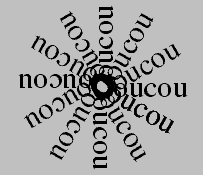
\includegraphics{round}%
%END IMAGE
%HEVEA\imageflush
\end{center}
\end{htmlout}
It is important to notice that things go smoothly because the
\verb+\usepackage{epsf}+ command  gets echoed to the
\filename{image} file.  In more complicated cases, \LaTeX{} may fail
on the \filename{image} file because it does not load the right
packages or define the right macros.


However, the above solution implies modifying the original \LaTeX{}
source code.
A better solution is to define the \verb+\epsfbox+
command, so that \hevea{} echoes  \verb+\epsfbox+ and its argument to
the image file and performs \verb+\imageflush+:
\begin{verbatim}
 \newcommand{\epsfbox}[1]{%
 \begin{toimage}
 \epsfbox{#1}
 \end{toimage}
 \imageflush}
\end{verbatim}
Such a definition must be seen by \hevea{} only. So, it is best put
in a separate file whose name is given as an extra argument on
\hevea{} command line (see section~\ref{heveaonly}).
Putting it in the document source
protected inside an \verb+%HEVEA+ comment is a bad idea, %
because it might then get echoed to the \textit{image} file
and generate trouble when \LaTeX{} is later run by \texttt{imagen}.

Observe that the above definition of \verb+\epsfbox+ is a definition
and not a redefinition (i.e., \verb+\newcommand+ is used and not
\verb+\renewcommand+),
because \hevea{} does not know about \verb+\epsfbox+ by default.
Also observe that this not a recursive definition, since
commands do not get expanded inside the \verb+toimage+ environment.

Finally, if the Postscript image is produced from a bitmap, it is
a pity to translate it back into a bitmap.
A better idea is first to generate a GIF file from the bitmap source
independantly
and then to include a link to that GIF file in \html{} output, see
section~\ref{imgsrc} for a description of this more adequate technique.


\subsection{Using filters}

Some programs extend \LaTeX{} capabilities using a filter principle.
In such a scheme, the document contains source fragments for the program.
A first run of the program on \LaTeX{} source changes these fragments
into constructs that \LaTeX{} (or a subsequent stage in the paper
document production chain, such as \texttt{dvips}) can handle.
Here again, the rule of the game is keeping \hevea{} away from the
normal process: first applying the filter, then making \hevea{} send
the filter output to the \filename{image} file, and then having
\texttt{imagen} do the job.


Consider the \texttt{gpic} filter, for making drawings.
Source for \texttt{gpic} is enclosed in \verb+.PS+\ldots \verb+.PE+,
then the result is available to subsequent \LaTeX{} source as a \TeX{}
box \verb+\box\graph+.
For instance the following source, from a \texttt{smile.tex} file,
draws a ``Smile!'' logo as a centered
paragraph:
\begin{verbatim}
 .PS
 ellipse "{\Large\bf Smile!}"
 .PE
 \begin{center}
 ~\box\graph~
 \end{center}
\end{verbatim}
Both the image description (\verb+.PS+\ldots\ \verb+.PE+) and usage (\verb+\box\graph+)
are for the \filename{image} file, and they should be
enclosed by \verb+%BEGIN IMAGE+\ldots\ \verb+%END IMAGE+ comments.
Additionally, the image link is put where it belongs by an
\verb+\imageflush+ command:
\begin{verbatim}
 %BEGIN IMAGE
 .PS
 ellipse "{\Large\bf Smile!}"
 .PE
 %END IMAGE
 \begin{center}
 %BEGIN IMAGE
 ~\box\graph~
 %END IMAGE
 %HEVEA\imageflush
 \end{center}
\end{verbatim}
The \texttt{gpic} filter is applied first, then come \texttt{hevea}
and \texttt{imagen}:
\begin{verbatim}
 # gpic -t < smile.tex > tmp.tex
 # hevea tmp.tex -o smile.html
 # imagen smile
\end{verbatim}
And we get:
\ifpdf
\begin{center}
\image{smile}
\end{center}
\else
%BEGIN IMAGE
.PS
ellipse "{\Large\bf Smile!}"
.PE
%END IMAGE
\begin{center}
%BEGIN IMAGE
~\box\graph~
%END IMAGE
%HEVEA\imageflush
\end{center}
\fi
Observe how the \verb+-o+ argument to \hevea{} is used and that
\texttt{imagen} argument is \hevea{} output basename (see
section~\ref{basenames} for the full definition of \hevea{} output basename).


In the \texttt{gpic} example, modifying user source cannot be totally avoided.
However, writing in a generic style saves typing.
For instance, users may define the following environment for
centered \texttt{gpic} pictures in \LaTeX{}:
\begin{verbatim}
 \newenvironment{centergpic}{}{\begin{center}~\box\graph~\end{center}}
\end{verbatim}
Source code will now be as follows:
\begin{verbatim}
 \begin{centergpic}
 .PS
 ellipse "{\Large\bf Smile!}"
 .PE
 \end{centergpic}
\end{verbatim}
\hevea{} will process this source correctly, provided it is given its
own definition for the \verb+centergpic+ environment beforehand:
\begin{verbatim}
 \newenvironment{centergpic}
   {\begin{toimage}}
   {\box\graph\end{toimage}\begin{center}\imageflush\end{center}}
\end{verbatim}
Assuming that the definition above is in a \ahref{\heveaurl/examples/smile.hva}{smile.hva} file,
the command sequence for translating
\ahref{\heveaurl/examples/smile.tex}{smile.tex} \mbox{now is}:
\begin{verbatim}
 # gpic -t < smile.tex > tmp.tex
 # hevea smile.hva tmp.tex -o smile.html
 tmp.tex:5: Warning: ignoring definition of \centergpic
 tmp.tex:5: Warning: not defining environment centergpic
 # imagen smile
\end{verbatim}
The warnings above are normal: they are issued when \hevea{} runs
across the \LaTeX{}-intended definition of the \verb+centergpic+
environment and refuses to override its own definition for that
environment.


\latexsection{Cutting your document into pieces with \hacha{}}
\pdfsection{Cutting your document into pieces with HaChA}
\label{hacha}
\hevea{} outputs a single \texttt{.html} file. This file can be
cut into pieces at various sectional units by {\hacha}

\subsection{Simple usage}
First generate your {\html} document by applying \hevea{}:
\begin{flushleft}
\texttt{\# hevea }\filename{mydoc}\texttt{.tex}
\end{flushleft}
Then cut \filename{mydoc}\texttt{.html} into pieces by the command:
\begin{flushleft}
\texttt{\# hacha }\filename{mydoc}\texttt{.html}
\end{flushleft}
This will generate a simple root file
\texttt{index.html}.
This root file holds document title, abstract and a simple table of
contents.
Every item in the table of contents contains a link to or into a file
that holds a ``cutting'' sectional unit.
By default, the cutting sectional unit is {\em section} in the
\filename{article} style and {\em chapter} in the \filename{book}
style.

Additionally, one level of sectioning below the cutting unit (i.e.,
subsections in the \filename{article} style and sections in the
\filename{book} style) is shown
as an entry in the table of contents.
Sectional units above the cutting section (i.e., parts in both
\filename{article} and \filename{book} styles) close the current table
of contents and open a new one.
Cross-references are properly handled, that is, the local links generated by
\hevea{} are changed into remote links.

The name of the root  file can be changed using the
\verb+-o+ option:
\begin{flushleft}
\texttt{\# hacha -o root.html }\filename{mydoc}\texttt{.html}
\end{flushleft}

Some of \hevea{} output get replicated in all the files generated by
\hacha{}.
Users can supply a header and a footer, which  will appear at the
begining and end of every page generated by \hacha{}. It suffices to
include the following commands in the document preamble:
\begin{flushleft}
\quad\verb+\htmlhead{+\textit{header}\verb+}+\\
\quad\verb+\htmlfoot{+\textit{footer}\verb+}+
\end{flushleft}
\hacha{} also makes every page it generates a clone of its input as
regards attributes to the \verb+<BODY ...>+ opening tag and
meta-information from the \verb+<HEAD>+\ldots{} \verb+<\HEAD>+
block. See section~\ref{metadef} for examples of this replication
feature.


\subsection{Advanced usage}

\hacha{} behavior can be altered from the document source, by using
a counter and a few macros.

A document that explicitly includes cutting macros still can be typeset by
\LaTeX{}, provided it loads the
\texttt{hevea.sty} style file from the \hevea{} distribution.
(See section~\ref{both} for details on this style file).
An alternative to loading the \texttt{hevea} package is to put
all cutting instructions in comments starting with \verb+%HEVEA+.



\subsubsection{Principle}
{\hacha} recognizes all sectional units, ordered as follows, from
top to bottom: {\em
part}, {\em chapter},
{\em section}, {\em subsection}, {\em subsubection},
\emph{paragraph} and \emph{subparagraph}.

At any point between \verb+\begin{document}+ and
\verb+\end{document}+,
there exist a current cutting sectional unit (cutting unit for short),
a current cutting depth, a root file and an output file.
Table of contents output goes to the root file, normal output goes to
the output file.
Cutting units start a new output file, whereas units comprised between the
cutting unit and the cutting units plus the cutting depth add new
entries in the table of contents.

At document start, the root file and the output file are {\hacha}
output file (i.e., \texttt{index.html}).
The cutting unit and the cutting depth are set to default values that
depend on the document style.

\subsubsection{Cutting macros}
The following cutting instructions are for use in the document
preamble. They command the cutting scheme of the whole document:
\comindex{cuttingunit}\comindex{tocnumber}\comindex{notocnumber}%
\countindex{cuttingdepth}%
\begin{description}
\item[{\tt\char92 cuttingunit}]
This is a macro that holds the document cutting unit. You can change
the default (which is {\em section} in the \filename{article} style
and {\em chapter} in the \filename{book} style)  by doing:
\begin{flushleft}
\verb+\renewcommand{\cuttingunit}{+{\it secname}\verb+}+.
\end{flushleft}
\item[{\tt\char92 tocnumber}] Instruct \hevea{} to put section numbers
into table of content entries.
\item[{\tt\char92 notocnumber}] Instruct \hevea{} \emph{not} to put
section numbers
into table of content entries. This is the default.
\item[{\tt cuttingdepth}]
This is a counter that holds the document cutting depth.
You can change the default value of 1 by doing
\verb+\setcounter{cuttingdepth}{+{\it numvalue}\verb+}+.
A cutting depth of zero means no other entries than the cutting units
in the table of contents.
\end{description}

Other cutting instructions are to be used after
\verb+\begin{document}+. They all generate \html{} comments in \hevea{}
output.
These comments then act as instructions to {\hacha}.
\comindex{cuthere}
\comindex{cutdef}
\comindex{cutend}
\begin{description}
\item[{\tt\char92 cuthere\{}{\it secname}{\tt\}\{}{\it itemtitle}{\tt\}}]
   Attempt a cut.
   \begin{itemize}
   \item If {\it secname} is the current cutting  unit or
   the keyword ``\texttt{now}'', then
   a new output file is started and an entry in the current table of contents
   is generated, with title {\it itemtitle}. This entry holds a link
   to the new output file.
   \item If {\it secname} is above the cutting  unit, then the
   current table of contents is closed. The output file is set to the
   current root file.
   \item If {\it secname} is below the cutting  unit and less than the
   cutting depth away from it, then an entry is added in the table of
   contents.
   This entry contains {\em itemtitle} and a link to the point where
   \verb+\cuthere+ appears.
   \item Otherwise, no action is performed.
   \end{itemize}

\item[{\tt\char92 cutdef[}{\it depth}{\tt]\{}{\it secname}{\tt \}}]
   Open a new table of contents, with cutting depth~{\em depth} and
   cutting unit {\em secname}. If the optional {\em depth} is absent,
   the cutting depth does not change.
   The output file becomes the root file.
   Result is unspecified if whatever {\em secname} expands to is
   a sectional unit name above
   the current cutting  unit, is not a valid sectional unit name or if
   {\em depth} does not expand to a small positive number.
\item[{\tt\char92 cutend}]
   End the current table of contents. This closes the scope of the
   previous \verb+\cutdef+. The cutting unit and cutting depth are
   restored.
   Note that \verb+\cutdef+ and \verb+\cutend+ must be properly balanced.
\end{description}

\noindent Default settings work as follows:
\verb+\begin{document}+ performs
\begin{verbatim}
\cutdef[\value{cuttingdepth}]{\cuttingunit}
\end{verbatim}
and \verb+\end{document}+
performs \verb+\cutend+.
All sectioning commands perform \verb+\cuthere+,
with the sectional unit name as first argument and the (optional, if
present) sectioning
command argument (i.e., the section title) as second argument.
Note that started versions of the sectioning commands also perform
cutting instructions.

\subsubsection{Examples}

Consider, for instance, a \filename{book} document with a long chapter
that you want to cut at the section level, showing subsections:
\begin{verbatim}
\chapter{A long chapter}
.....

\chapter{The next chapter}
\end{verbatim}
\comindex{cutdef}\comindex{cutend}
Then, you should insert a \verb+\cutdef+ at chapter start and a
\verb+\cutend+ at chapter end:
\begin{verbatim}
\chapter{A long chapter}
%HEVEA\cutdef[1]{section}
.....
%HEVEA\cutend
\chapter{The next chapter}
\end{verbatim}
Then, the file
that would otherwise contain the long chapter now contains the chapter
title and a table of sections.
No other change is needed, since the macro \verb+section+ already
performs the appropriate \verb+\cuthere{section}{...}+ commands,
which were ignored by default.
(Also note that cutting macros are placed inside \verb+%HEVEA+ comments,
for \LaTeX{} not to be disturbed).

\comindex{cuthere}
\comindex{cuttingunit}
The \verb+\cuthere+ macro can be used to put some document parts into
their own file.
This may prove appropriate for long cover pages or abstracts that would
otherwise go into the root file.
Consider the following document:
\begin{verbatim}
\documentclass{article}

\begin{document}

\begin{abstract} A big abstract \end{abstract}
...
\end{verbatim}
Then, you make the abstract go to its own file as it was a cutting
unit by typing:
\begin{verbatim}
\documentclass{article}
\usepackage{hevea}

\begin{document}
\cuthere{\cuttingunit}{Abstract}
\begin{abstract} A big abstract \end{abstract}
...
\end{verbatim}
(Note that, this time, cutting macros appear unprotected in the
source. However, \LaTeX{} still can process the document, since the
\texttt{hevea} package is loaded).

\subsection{More Advanced Usage}
In this section we show how to alter some details of \hacha{}
behavior.
This includes controling output file names and the title of generated
web pages and introducing arbitrary cuts.

\subsubsection{Controlling output file names}\label{cutname}
\cutname{cutname.html}
\comdefindex{cutname}
When invoked as \texttt{hacha \textit{doc}.html},
\hacha{} produces a \texttt{index.html} table of links file that
points into \textit{doc}\texttt{001.html},
\textit{doc}\texttt{002.html}, etc. content files.
This is not very convenient when one wishes to point inside the
document from outside.
However, the \verb+\cutname{+\textit{name}\verb+}+ command
sets the name of  the current output file name as \textit{name}.

Consider a document cut at the section level, which contains the
following important section~:
\begin{verbatim}
\section{Important section}\label{important}
...
\end{verbatim}
To make the important section goes into file \texttt{important.html},
one writes~:
\begin{verbatim}
\section{Important section}\label{important}\cutname{important.html}
...
\end{verbatim}
Then, section ``Important section'' can be referenced from
an \hevea{} unaware \html{} page by~:
\begin{verbatim}
In this document, there is a very
<A HREF="important#important.html">important section</A>.
\end{verbatim}
\ifhevea
If you are reading the \html{} version of this manual, you may check
that wou are now reading file ``\texttt{cutname.html}''.
This particular file name has been specified from the source
using \verb+\cutname{cutname.html}+.
\fi

\subsubsection{Controlling page titles}
\comdefindex{htmlprefix}
When \hacha{} creates a web page from a given sectional unit,
the title of this page normally is the name of the sectional unit.
For instance, the title of this very page should be
``Cutting your document into pieces with \hacha''.
It is possible to insert some text at the beginning of all page
titles, by using the \verb+\htmlprefix+ command.
Hence, by writing
\verb+\htmlprefix{\hevea{} Manual: }+ in the document,
the title of this page would become~:
``\hevea{} Manual: Cutting your document into pieces with \hacha''
and the title of all other pages would show the same prefix.

\subsubsection{Links for the root file}
\comdefindex{toplinks}
The command \verb+\toplinks{+\textit{prev}\verb+}{+\textit{up}\verb+}{+\textit{next}\verb+}+ instructs \hacha{}  to put links to a
``previous'', ``up'' and ``next'' page in the root file.
The following points are worth noticing:
\begin{itemize}
\item The \verb+\toplink+ command must appear in the document preamble
(i.e., before \verb+\begin{document}+).
\item The arguments
\textit{prev}, \textit{up} and \textit{next} should expand to url's,
notice that these argument are processed (see section~\ref{urlareprocessed}).
\item When one of the expected argument is left empty,
the corresponding link is not generated.
\end{itemize}
This feature can prove useful to
relate documents that are generated independantly by
\hevea{} and \hacha{}.


\subsubsection{Cutting a document anywhere}
\envdefindex{cutflow}
Part of a document goes to a separate file whem enclosed in a
\verb+cutflow+ environment~:
\begin{flushleft}
  \verb+\begin{cutflow}{+\textit{title}\verb+}+\ldots\verb+\end{cutflow}+
\end{flushleft}

\noindent The content ``\ldots'' will go into a file of its
own, while
the argument \textit{title} is used as the title of the introduced
\html{} page.

The \html{} page introduced here does not belong to the normal flow of
text.
Consequently, one needs an explicit reference from the normal flow of text
into the content of the \verb+cutflow+ environment.
This will occur naturally when the content of the \verb+cutflow+ environment.
contains a \verb+\label+ construct.
This look natural in the following quiz example:
\begin{verbatim}
\paragraph{A small quiz}
\begin{enumerate}
\item What is black?
\item What is white?
\item What is Dylan?
\end{enumerate}
Answers in section~\ref{answers}.
\begin{cutflow}{Answers}
\paragraph{Quiz answers}\label{answers}
\begin{enumerate}
\item Black is black.
\item White is white.
\item Dylan is Dylan.
\end{enumerate}
\end{cutflow}
\end{verbatim}
\ifhevea The example yields:
\paragraph{A small quiz}
\begin{enumerate}
\item What is black?
\item What is white?
\item What is Dylan?
\end{enumerate}
Answers in section~\ref{answers}.
\begin{cutflow}{Answers}
\paragraph{Quiz answers}\label{answers}
\begin{enumerate}
\item Black is black.
\item White is white.
\item Dylan is Dylan.
\end{enumerate}
\end{cutflow}
\fi

\comindex{aname}\comindex{ahrefloc}
However,introducing \html{} hyperlink targets and
references with the \verb+\aname+ and \verb+\ahrefloc+ commands
(see section~\ref{hyperlink})
will be more practical most of the time.




\latexsection{Generating \html{} constructs}
\pdfsection{Generating HTML constructs}
\hevea{} output language being \html{}, it is normal for users to insert
hypertext constructs their documents, or to control colors.

\subsection{High-Level Commands}
\hevea{} provides high-level commands for doing this.
Users are advised to use these macros in the first place,
because it is easy to write incorrect \html{} and that writting
\html{} directly may interfeer in nasty ways with \hevea{} internals.


\subsubsection{Commands for Hyperlinks}\index{hyperlinks}\label{hyperlink}
A few commands for hyperlink  management and included images
are provided, all these
commands have approriate equivalents defined by the \texttt{hevea}
package (see section~\ref{heveastyle}).
Hence, a document that relies on these high-level commands
still can be typeset by \LaTeX{}, provided it loads the \texttt{hevea}
package.

\comindex{ahref}\comindex{ahrefurl}\comindex{footahref}\comindex{ahrefloc}
\comindex{aname}
\comindex{mailto}
\comindex{imgsrc}
\comindex{home}
%BEGIN LATEX
\bigskip
%END LATEX
\begin{tabular}{l<{\qquad}p{.3\linewidth}@{\qquad}p{.3\linewidth}}
\multicolumn{1}{c}{Macro} & \multicolumn{1}{c}{\hevea} &
\multicolumn{1}{c}{\LaTeX}\\
\hline

\verb+\ahref{+\textit{url}\verb+}{+\textit{text}\verb+}+ &
make \textit{text} an hyperlink to \textit{url} &
echo \textit{text}\\ \hline

\verb+\footahref{+\textit{url}\verb+}{+\textit{text}\verb+}+ &
make \textit{text} an hyperlink to \textit{url} &
make \textit{url} a footnote to \textit{text},
\textit{url} is shown in typewriter font\\ \hline

\verb+\ahrefurl{+\textit{url}\verb+}+ &
make \textit{url} an hyperlink to \textit{url}.
&
typeset \textit{url} in typewriter font\\ \hline

\verb+\ahrefloc{+\textit{label}\verb+}{+\textit{text}\verb+}+ &
make \textit{text} an hyperlink to \textit{label} inside the document
&
echo \textit{text}\\ \hline

\verb+\aname{+\textit{label}\verb+}{+\textit{text}\verb+}+ &
make \textit{text} an hyperlink target with label \textit{label} &
echo \textit{text}\\ \hline

\verb+\mailto{+\textit{address}\verb+}+ &
make \textit{address} a ``mailto'' link to \textit{address} &
typeset \textit{address} in typewriter font
\\ \hline
\verb+\imgsrc[+\textit{attr}\verb+]{+\textit{url}\verb+}+
& insert \textit{url} as an image, \textit{attr} are attributes in the
\html{} sense & do nothing \\ \hline
\verb+\home{+\textit{text}\verb+}+ &
\multicolumn{2}{p{.6\linewidth}}{produce a home-dir url both for output and links, output aspect is: ``\home{\textit{text}}''}
\end{tabular}

\label{urlareprocessed}It is important to notice that all arguments
are processed.
For instance, to insert a link to
my home page, (\verb+http://pauillac.inria.fr/~maranget/index.html+),
you should do something like this~:
\begin{verbatim}
\ahref{http://pauillac.inria.fr/\home{maranget}/index.html}{his home page}
\end{verbatim}

Given the frequency of \verb+~+, \verb+#+ etc. in urls,
this is annoying. Moreover, the immediate solution, using \verb+\verb+,
\verb+\ahref{\verb" ... /~maranget/..."}{his home page}+ does not
work, since \LaTeX{} forbids verbatim formatting inside command arguments.

\comindex{url}
Fortunately, the \texttt{url} package provides a very convenient
\verb+\url+ command that acts like \verb+\verb+ and can appear in
other command arguments
(unfortunately, this is not the full story, see section~\ref{urlpackage}).
Hence, provided the \texttt{url} package is loaded,
a more convenient reformulation of the example above is~:
\begin{verbatim}
\ahref{\url{http://pauillac.inria.fr/~maranget/index.html}}{his home page}
\end{verbatim}
Or even better~:
\begin{verbatim}
\urldef{\lucpage}{\url}{http://pauillac.inria.fr/~maranget/index.html}
\ahref{\lucpage}{his home page}
\end{verbatim}
It may seem complicated, but this is a safe way to have a
document processed both by \LaTeX{} and \hevea{}.
Drawing a line between url typesetting and hyperlinks is correct,
because users may sometime want urls to be processed and some other
times not.
Moreover, \hevea{} (optionnaly) depends on only one third party package:
\texttt{url}, which as correct as it can be and well-written.



\comindex{oneurl}
\comindex{footurl}
In case the \verb+\url+ command is undefined
at the time \verb+\begin{document}+ is processed, the commands
\verb+\url+, \verb+\oneurl+ and \verb+\footurl+ are defined as
synonymous for
\verb+\ahref+, \verb+\ahrefurl+ and \verb+\footahref+, thereby
ensuring
some compatibility with older versions of \hevea.
Note that this usage of \verb+\url+ is deprecated.

\subsubsection{\html{} style colors}\label{color:high}
Specifying colors both for \LaTeX{} and
\hevea{} should be done using the \texttt{color} package (see
section~\ref{color:package}).
However,one can also specify text color using special type style declarations.
The \texttt{hevea.sty} style file
define no equivalent for these declarations, which therefore are for
\hevea{} consumption only.

Those declarations follow \html{} conventions for colors.
There are sixteen predefined colors:
\begin{center}
\begin{tabular}{p{.7\linewidth}}
%HEVEA\black
\verb+\black+,
%HEVEA\silver
\verb+\silver+,
%HEVEA\gray
\verb+\gray+,
%HEVEA\white
\verb+\white+,
%HEVEA\maroon
\verb+\maroon+,
%HEVEA\red
\verb+\red+,
%HEVEA\fuchsia
\verb+\fuchsia+,
%HEVEA\purple
\verb+\purple+,
%HEVEA\green
\verb+\green+,
%HEVEA\lime
\verb+\lime+,
%HEVEA\olive
\verb+\olive+,
%HEVEA\yellow
\verb+\yellow+,
%HEVEA\navy
\verb+\navy+,
%HEVEA\blue
\verb+\blue+,
%HEVEA\teal
\verb+\teal+,
%HEVEA\aqua
\verb+\aqua+
\end{tabular}
\end{center}
\comindex{htmlcolor}Additionally, the current text color can be
changed by the declaration \verb+\htmlcolor{+{\it number}\verb+}+,
where {\it number} is a six digit hexadecimal number specifying a
color in the RGB space.  For instance, the following declarations
change font color to dark gray:%HEVEA{\htmlcolor{404040}%
\begin{verbatim}
  \htmlcolor{404040}
\end{verbatim}
%HEVEA}

\subsection{More on included images}\label{imgsrc}
\index{image inclusion!in GIF}\comindex{imgsrc}
The \verb+\imgsrc+ command
becomes handy when one has images both in Postscript and GIF format.
As explained in section~\ref{substimage}, Postscript images can
be included in \LaTeX{} documents by using the \verb+\epsfbox+
command from the \texttt{epsf} package.
For instance, if \texttt{screenshot.ps} is an encapsulated  Postscript
file, then a \texttt{doc.tex} document can include it by:
\begin{verbatim}
\epsfbox{screenshot.ps}
\end{verbatim}
We may very well also have a GIF version of the screenshot image
(or be able to produce one easily using image converting tools),
let us store it in a \texttt{screenshot.ps.gif} file.
Then, for \hevea{} to include a link to the GIF image in its
output, it suffices
to define the \verb+\epsfbox+ command in the \texttt{macro.hva} file
as follows:
\begin{verbatim}
\newcommand{\epsfbox}[1]{\imgsrc{#1.gif}}
\end{verbatim}
Then \hevea{} has to be run as:
\begin{verbatim}
# hevea macros.hva doc.tex
\end{verbatim}
Since it has its own definition of \verb+\epsfbox+, \hevea{} will
silently include a link the GIF image and not to the Postscript image.

If another naming scheme for image files is prefered, there are
alternatives.
For instance, assume that Postscript files are of the kind
\textit{name}\texttt{.ps}, while GIF files are of the kind
\textit{name}\texttt{.gif}.
Then, images can be included using
\verb+\includeimage{+\textit{name}\verb+}+, where
\verb+\includeimage+ is a specific user-defined command:
\begin{verbatim}
\newcommand{\includeimage}[1]{\ifhevea\imgsrc{#1.gif}\else\epsfbox{#1.ps}\fi}
\end{verbatim}
Note that this method uses the \texttt{hevea} boolean register (see
section~\ref{heveabool}).
If one does not wish to load the \texttt{hevea.sty} file,
one can adopt the slightly more verbose definition:
\begin{verbatim}
\newcommand{\includeimage}[1]{%
%HEVEA\imgsrc{#1.gif}%
%BEGIN LATEX
\epsfbox{#1.ps}
%END LATEX
}
\end{verbatim}
When the Postscript file has been produced by
translating a bitmap file, this simple method of making a GIF image and
using the \verb+\imgsrc+ command 
is the most adequate.
It should be prefered over using the more automated \textit{image} file
mechanism (see section~\ref{imagen}),
which will translate the image back from
Postscript to bitmap format and will thus degrade it.



\subsection{The \texttt{rawhtml} environment}\label{rawhtml}
\envindex{rawhtml}\comindex{rawhtmlinput}
Any text enclosed between \verb+\begin{rawhtml}+ and
\verb+\end{rawhtml}+ is echoed verbatim into the \html{} output file.
Similarily, \verb+\rawhtmlinput{+\textit{file}\verb+}+ echoes the
contents of file~\textit{file}.

For avoiding to break \html~element nesting, the \texttt{rawhtml}
environment should be used only at toplevel (i.e. not within another
environment), and it should contain only \html~text that makes sense
alone. For instance, writing
\verb+\begin{rawhtml}<TABLE><ALIGN=right>\end{rawhtml}+\ldots{}
\verb+\begin{rawhtml}</TABLE>\end{rawhtml}+ is
dangerous, because \hevea{} is not informed about opening and closing
the block-level element \texttt{TABLE}. In that case, one should use
the internal macros \verb+\@open+ and \verb+\@close+ of the following
section.


When \hevea{} is given the command line option ``\texttt{-O}'',
checking and optimization of text-level elements in the whole document
takes place.  As a consequence, incorrect \html{} introduced by using
the \texttt{rawhtml} environment may be detected at a later stage.



For the document to remain processable by \LaTeX{}, it must load the
\texttt{hevea.sty} style file (see section~\ref{heveastyle}).

\subsection{Internal macros}\label{internal}
In this section a few of \hevea{} internal macros are
described.
Internal macros occur at the final expansion stage of \hevea{} and
invoke Objective Caml code.

Normally, user source code should not use them, since
their behavior may change from one version of \hevea{} to another and
because using them incorrectly easily
crashes \hevea.
However:
\begin{itemize}
\item Internal macros
are almost mandatory for writing supplementary base style files.
\item Casual usage is a convenient (but dangerous) way to finely control
output (cf. the examples in the next section).
\item Knowing a little about internal macros helps in understanding how
\hevea{} works.
\end{itemize}


\index{block-level elements}
The general principle of \hevea{} is that \LaTeX{} environments
\verb+\begin{+\textit{env}\verb+}+\ldots{}
\verb+\end{+\textit{env}\verb+}+ get
translated into \html{} block-level elements \verb+<+\textit{block}
\textit{attributes}\verb+>+\ldots{} \verb+</+\textit{block}\verb+>+.
More specifically, such block level elements are opened by the
internal macro \verb+\@open+ and closed by the internal macro
\verb+\@close+.
As a special case, \LaTeX{} groups \verb+{+\ldots{} \verb+}+
get translated into \html{} \emph{groups}, which are shadow block-level
elements with neither opening tag nor closing tag.

\index{"@print@\texttt{\char92"@print}|defocc}
\index{"@getprint@\texttt{\char92"@getprint}|defocc}
\index{"@hr@\texttt{\char92"@hr}|defocc}
\index{"@open@\texttt{\char92"@open}|defocc}
\index{"@close@\texttt{\char92"@close}|defocc}
\index{"@style@\texttt{\char92"@style}|defocc}
\index{"@styleattr@\texttt{\char92"@styleattr}|defocc}
\index{"@nostyle@\texttt{\char92"@nostyle}|defocc}
\index{"@clearstyle@\texttt{\char92"@clearstyle}|defocc}
\index{"@fontsize@\texttt{\char92"@fontsize}|defocc}
\index{"@fontcolor@\texttt{\char92"@fontcolor}|defocc}
It is important to notice that primitive arguments \emph{are}
processed (except for the \verb+\@print+ primitive, and for some of
the basic style primitives). Thus,
some characters cannot be given directly (e.g. \verb+#+ and
\verb+%+ must be given as \verb+\#+ and \verb+\%+).
\begin{description}
\item[{\tt\char92 @print\char123}{\it text}{\tt\char125}]
Echo \textit{text} verbatim.
\item[{\tt\char92 @getprint\char123}{\it text}{\tt\char125}]
Process \textit{text} using a special output mode that strips off
\html~tags. This macro is the one to use for processed attributes of
\html~tags.
\item[{\tt\char92 @hr[}{\it attr}{\tt]\char123}{\it
width}{\tt\char125\char123}{\it height}{\tt\char125}]
Ouput an \html{} horizontal rule, \textit{attr} is attributes given
directly (e.g. \verb+SIZE=3 HOSHADE+), while \textit{width} and
\textit{height} are length arguments given in the \LaTeX{} style
(e.g. \verb+2pt+ or~\verb+.5\linewidth+).



\item[{\tt\char92 @open\char123}{\it BLOCK}{\tt\char125\char123}{\it
attributes}{\tt\char125}]
Open \html{} block-level element \textit{BLOCK} with attributes
\textit{attributes}. The block name \textit{BLOCK} \emph{must} be
uppercase.
As a special case \textit{BLOCK} may be the empty string, then a \html{}
\emph{group} is opened.
\item[{\tt\char92 @close\char123}{\it BLOCK}{\tt\char125}]
Close \html{} block-level element \textit{BLOCK}.
Note that \verb+\@open+ and \verb+\@close+ must be properly balanced.
\end{description}

\index{text-level elements}
Text-level elements are managed differently. They are not seen
as blocks that must be closed explicitely and they are replaced by the
internal text-level declarations \verb+\@style+ (and
\verb+\@styleattr+), \verb+\@fontsize+ and
\verb+\@fontcolor+. Block-level elements (and \html{} groups)
delimit the effect of such declarations.
\begin{description}
\item[{\tt\char92 @style\char123}{\it SHAPE}{\tt\char125}]
Declare the text shape \textit{SHAPE} (which must be uppercase)
as active. Text shapes are known as font style elements (\verb+I+, \verb+TT+,
etc.) or phrase elements (\verb+EM+, etc.) in the
\html{} terminology, they are part of the more general class of
text-level elements.

The text-level element {\it SHAPE} will get opened as soon as
necessary and closed automatically, when the
enclosing block-level elements get closed.
Enclosed block-level elements are treated properly by closing {\it
SHAPE} before them, and re-opening {\it SHAPE} inside them.
The next text-level constructs exhibit similar behavior with respect
to block-level elements.
\item[{\tt\char92 @styleattr\char123}{\it NAME}{\tt\char125\char123}{\it
attr}{\tt\char125}]\index{text-level elements!SPAN}
Declare the text-level element \textit{NAME} with
attribute~\textit{attr}
active. This primitive behaves as \verb+\@style+, except that the
opennig tag has attributes.
This primitive may prove useful for introducing \texttt{SPAN} elements.
Note that neither argument is processed.
\item[{\tt\char92 @fontsize\char123}{\it int}{\tt\char125}]
Declare the text-level element \verb+FONT+ with attribute
\verb+SIZE=+\textit{int} as active. Note that \textit{int} must
be a small integer in the range \texttt{1},\texttt{2}, \ldots{} , \texttt{7}.
\item[{\tt\char92 @fontcolor\char123}{\it color}{\tt\char125}]
Declare the text-level element \verb+FONT+ with attribute
\verb+COLOR=+\textit{color} as active.
Note that \textit{color} must be a color attribute value in the \html{}
style. That is either one of the sixteen conventional colors
\verb+black+, \verb+silver+ etc, or a RGB hexadecimal color specification
of the form
\verb+"#+\textit{XXXXXX}\verb+"+ (yes, quotes are needed).
Note that the argument \textit{color} is processed, as a consequence
numerical color arguments should be given as \verb+"\#+\textit{XXXXXX}\verb+"+.

\item[{\tt\char92 @nostyle}]
Close active text-level declarations and ignore further text-level
declarations.
The effect stops when the enclosing block-level element is closed.
\item[{\tt\char92 @clearstyle}]
Simply close active text-level declarations.
\end{description}

\subsection{Examples}
\comindex{purple}
\index{"@open@\texttt{\char92"@open}}
\index{"@close@\texttt{\char92"@close}}
As a first example of using internal macros, consider the following
excerpt from the \texttt{hevea.hva} file that
defines the \LaTeX{} \verb+center+ environment:
\begin{verbatim}
\newenvironment{center}{\@open{DIV}{ALIGN=center}}{\@close{DIV}}
\end{verbatim}
Another example is the definition of the \verb+\purple+
color declaration (see section~\ref{color:high}):
\begin{verbatim}
\newcommand{\purple}{\@fontcolor{purple}}
\end{verbatim}

\hevea{} does not feature all text-level elements by default.
However one can easily use them with the internal macro
\verb+\@style+.
For instance this is how you can make all emphasized text blink:
\begin{verbatim}
\renewcommand{\em}{\@style{EM}\@style{BLINK}}
\end{verbatim}

\comindex{imgsrc}
\index{"@print@\texttt{\char92"@print}}
\index{"@getprint@\texttt{\char92"@getprint}}
\index{"@nostyle@\texttt{\char92"@nostyle}}
Then, here is the definition of a simplified \verb+\imgsrc+
command (see section~\ref{hyperlink}), without its optional argument:
\begin{verbatim}
\newcommand{\imgsrc}[1]
  {\@print{<IMG SRC="}\@getprint{#1}\@print{">}}
\end{verbatim}
Here, \verb+\@print+ and \verb+\@getprint+ are used to output
\html~text, depending upon wether this text requires processing or not.
Note that \verb+\@open{IMG}{SRC="#1"}+ is not correct,
because the element \verb+IMG+ consists in a single tag, without a
closing tag.

\index{"@nostyle@\texttt{\char92"@nostyle}}
Another interesting example is the definition of the command
\verb+\@doaelement+,
which \hevea{} uses internaly to output \texttt{A} elements.
\begin{verbatim}
\newcommand{\@doaelement}[2]
  {{\@nostyle\@print{<A }\@getprint{#1}\@print{>}}{#2}{\@nostyle\@print{</A>}}
\end{verbatim}
The command \verb+\@doaelement+ takes two arguments: the first
argument contains the opening tag attributes; while the second element is
the textual content of the \verb+A+ element.
By contrast with the \verb+\imgsrc+ exemple above,
tags are emitted inside groups where styles are canceled by using the
\verb+\@nostyle+ declaration.
Such a complication is needed, so as to avoid breaking proper nesting
of text-level elements.

\label{getcolor:usage}
\envindex{bgcolor}
\index{"@open@\texttt{\char92"@open}}
\index{"@close@\texttt{\char92"@close}}
Finally, here is an example of direct block opening.
The \texttt{bgcolor} environment from the \texttt{color} package
locally changes background color (see section~\ref{bgcolor}).
This environment is defined as follows:
\begin{verbatim}
\newenvironment{bgcolor}[2][CELLPADDING=10]
  {\@open{TABLE}{#1}\@open{TR}{}\@open{TD}{BGCOLOR=\@getcolor{#2}}}
  {\@close{TD}\@close{TR}\@close{TABLE}}
\end{verbatim}
The \texttt{bgcolor} environment operates by opening a \html{} table
(\verb+TABLE+) with only one row (\verb+TR+) and cell (\verb+TD+) in
its opening command, and closing all these elements in its closing
command. In my opinion, such a style of opening block-level elements
in environment opening commands and closing them in environment
closing commands is good style.

Notice that, the \texttt{hevea} package provides a tentative
definition of the \texttt{bgcolor} environment. As a consequence and
provided the \texttt{hevea} package is loaded, documents that use the
\texttt{bgcolor} environment remain processable by \LaTeX{}.


\index{"@getcolor@\texttt{\char92"@getcolor}}
The one cell background color is forced with a \verb+BGCOLOR+
attribute.
Note that the mandatory argument to \verb+\begin{bgcolor}+ is the
background color expressed as a high-level color, which therefore
needs to be translated into a low-level color by using the
\verb+\@getcolor+ internal macro from the \texttt{color} package.
Additionally,  \verb+\begin{bgcolor}+ takes \html{} attributes
as an optional argument. These attributes are the ones of the
\verb+TABLE+ element.

\latexsection{Customizing \hevea}
\pdfsection{Customizing HeVeA}
\hevea{} can be controlled by writing \LaTeX{} code. In this section,
we examine how users can change \hevea{} default behavior or add
functionalities. In all this section we assume that a document
\texttt{mydoc.tex} is processed, using a private command file
\texttt{macros.hva}. That is, \hevea{} is invoked as:
\begin{verbatim}
# hevea macros.hva mydoc.tex
\end{verbatim}
The general idea is as follows: one redefines \LaTeX{} constructs in
\texttt{macros.hva}, using internal commands. This requires a good
working knowledge of both \LaTeX{} and \html.
Usually, one can avoid internal commands, but then, all command
redefinitions interact, sometimes in very nasty ways.


\subsection{Simple changes}
Users can easily change the rendering of some constructs. For
instance, assume that \emph{all} quotations in a text should be
emphasized. Then, it suffices to put the following redeclaration in
\texttt{macros.hva}:
\begin{verbatim}
\renewenvironment{quote}
  {\@open{BLOCKQUOTE}{}\@style{EM}}
  {\@close{BLOCKQUOTE}}
\end{verbatim}

The same effect can be achieved without using any of the internal
commands:
\begin{verbatim}
\let\oldquote\quote
\let\oldendquote\endquote
\renewenvironment{quote}{\oldquote\em}{\oldendquote}
\end{verbatim}
In some sense, this second 
solution is easier, when one already knows
how to customize \LaTeX{}. However, this is less safe, since the definition of
\verb+\em+ can be changed elsewhere.

\subsection{Changing defaults for type-styles}\label{customize-style}

\hevea{} default rendering of type style changes is described in
section~\ref{type-style}.
For instance, the following example shows the default rendering
for the font shapes:
\begin{verbatim}
\itshape italic shape \slshape slanted shape
\scshape small caps shape \upshape upright shape
\end{verbatim}
By default, \verb+\itshape+ is italics, \verb+\slshape+ is maroon
italics, \verb+\scshape+ is navy blue color and \verb+\upshape+ is no
style at all.
All shapes are mutually exclusive, this means that each shape
declaration cancels the effect of other active shape declarations.
For instance, in the example, small caps shapes is navy blue and not
navy blue italics.
\begin{htmlonly}
\begin{htmlout}
\itshape italic shape \slshape slanted shape
\scshape small caps shape \upshape upright shape
\end{htmlout}
\end{htmlonly}

If one wishes to change the rendering of some of the shapes (say small
caps), then one should redefine the old-style \verb+\sc+ declaration.
For instance, to render small caps as bold fonts, one should
redefine \verb+\sc+ by \verb+\renewcommand{\sc}{\@style{B}}+ in
\texttt{macros.hva}.


\begin{htmlonly}
And now, the shape example above gets rendered as follows:
\begin{htmlout}\renewcommand{\sc}{\@style{B}}
{\itshape italic shape \slshape slanted shape
\scshape small caps shape \upshape upright shape}
\end{htmlout}

Redefining the old-style \verb+\sc+ is compatible with the cancelation
mechanism, redefining \verb+\scshape+ is not.
Thus, redefining directly \LaTeXe{} \verb+\scshape+ with
\verb+\renewcommand{\scshape}{\@style{B}}+ would yield:
\begin{htmlout}\renewcommand{\scshape}{\@style{B}}
{\itshape italic shape \slshape slanted shape
\scshape small caps shape \upshape upright shape}
\end{htmlout}
\end{htmlonly}

Hence, redefining old-style declarations using internal commands
should yield satisfactory output.
However, since cancelation is done at the \html{}
level, a declaration belonging to one component may sometimes cancel the
effect of another that belongs to another component.
Anyway, you might have not noticed it if I had not told you.

\subsection{Changing the interface of a command}\label{customize-let}
Assume for instance that the base style of \texttt{mydoc.tex} is
\textit{jsc} (the
\emph{Journal of Symbolic Computation} style for articles).
For running \hevea{}, the \textit{jsc} style can be replaced by
\textit{article}
style, but for a few commands whose calling interface is changed.
In particular, the \verb+\title+ command
takes an extra optional argument (which \hevea{} should ignore
anyway).
However, \hevea{} can process the document as it stands.
One  solution to insert the following lines into \texttt{macros.hva}:
\begin{verbatim}
\newcounter {part}
\newcounter {section}
\newcounter {subsection}[section]
\newcounter {subsubsection}[subsection]
\newcounter {paragraph}[subsubsection]
\newcounter {subparagraph}[paragraph]
\renewcommand \thepart {\Alph{part}}
\renewcommand\thesubsection   {\thesection.\arabic{subsection}}
\renewcommand\thesubsubsection{\thesubsection .\arabic{subsubsection}}
\renewcommand\theparagraph    {\thesubsubsection.\arabic{paragraph}}
\renewcommand\thesubparagraph {\theparagraph.\arabic{subparagraph}}

\newcounter{figure}

\newcommand{\partname}{Part}
\newcommand{\chaptername}{Chapter}
\newcommand{\part}[1]{%
  \@open{H1}{ALIGN=center}
  \stepcounter{part}
  \partname:~\thepart\\
  #1
  \@close{H1}
}
\newcommand{\part*}[1]{%
  \@open{H1}{ALIGN=center}
  #1
  \@close{H1}
}

\newcommand{\section}[1]{%
  \@open{H2}{}
  \stepcounter{section}
  \thesection~
  #1
  \@close{H2}
}
\newcommand{\section*}[1]{%
  \@open{H2}{}
  #1
  \@close{H2}
}


\newcommand{\subsection}[1]{%
  \@open{H3}{}
  \stepcounter{subsection}
  \thesubsection~
  #1
  \@close{H3}
}
\newcommand{\subsection*}[1]{%
  \@open{H3}{}
  #1
  \@close{H3}
}


\newcommand{\subsubsection}[1]{%
  \@open{H4}{}
%  \stepcounter{subsubsection}
%  \thesubsubsection~
  #1
  \@close{H4}
}
\newcommand{\subsubsection*}[1]{%
  \@open{H4}{}
  #1
  \@close{H4}
}

\newcommand{\paragraph}[1]{%
  \@open{H5}{}
%  \stepcounter{paragraph}
%  \theparagraph~
  #1
  \@close{H5}
}
\newcommand{\paragraph*}[1]{%
  \@open{H5}{}
  #1
  \@close{H5}
}

\newenvironment{thebibliography}[1]{\section*{\bibname}\@open{DL}{}}{\@close{DL}}
\newcommand{\bibitem}[1]{\item[{\purple[\@bibref{#1}]\label{#1}}]}
% Force document class ``article''
\let\oldtitle=\title
\renewcommand{\title}[2][]{\oldtitle{#2}}
\end{verbatim}
The effect is to replace \verb+\title+ by a new command which
calls \hevea{} \verb+\title+ with the appropriate argument.
\subsection{Checking the optional argument within a command}\label{fullepsfbox}
\index{image inclusion!in Postcript}
\hevea{} fully implements \LaTeXe{} \verb+\newcommand+.
That is, users can define commands with an optional argument.
Such a feature permits to write a \verb+\epsfbox+ command that
has the same interface as the \LaTeX{} command and
echoes itself as it is invoked to the \textit{image} file.
To do this, the \hevea{} \verb+\epsfbox+ command has to check
whether it is invoked with an optional argument or not.
This can be achieved as follows~:
\begin{verbatim}
\newcommand{\epsfbox}[2][!*!]{%
\ifthenelse{\equal{#1}{!*!}}
{\begin{toimage}\epsfbox{#2}\end{toimage}}%No optional argument
{\begin{toimage}\epsfbox[#1]{#2}\end{toimage}}}%With optional argument
\imageflush}
\end{verbatim}

\subsection{Changing the Format of Images}
\index{image inclusion!output format}
\index{PNG}
\comindex{imageflush}
\comindex{imgsrc}
Semi-automatic generation of included images is described in
section~\ref{imagen}.

Links to included images are generated by the \verb+\imageflush+
command, which calls the \verb+\imgsrc+ command~:
\begin{verbatim}
\newcommand{\imageflush}[1][]
{\@imageflush\stepcounter{image}\imgsrc[#1]{\hevaimagedir\jobname\theimage\heveaimageext}}
\end{verbatim}
That is, you may supply a \html-style attribute to the included image,
as an optional argument to the \verb+\imageflush+ command.


By default, images are GIF images, stored in ``\texttt{.gif}'' files.
\hevea{} provides direct support for the alternative PNG image file
format.
It suffices to invoke \texttt{hevea} as:
\begin{flushleft}
\texttt{\#~hevea~png.hva}~\textit{mydoc.tex}
\end{flushleft}

Then imagen must be run as:
\begin{flushleft}
\texttt{\#~imagen~-png}~\textit{mydoc}
\end{flushleft}

A convenient alternative is to invoke \texttt{hevea} as:
\begin{flushleft}
\texttt{\#~hevea~-fix~~png.hva}~\textit{mydoc.tex}
\end{flushleft}
Then \texttt{hevea} will invoke \texttt{imagen} with the appropriate
option when it thinks images need to be rebuild.


\subsection{Storing images in a separate directory}
\comindex{heveaimagedir}
By redefining the \verb+heveaimagedir+ command, users can specify a
directory for images.

More precisely, if the following redefinition occurs in the document
preamble.
\begin{flushleft}
\verb+\renewcommand{\heveaimagedir}{+\textit{dir}\verb+}+
\end{flushleft}
Then, all links to images in the produced \HTML{} file will be as
``\textit{dir}/\ldots''.
Then \texttt{imagen} must be invoked as:
\begin{flushleft}
\texttt{\#~imagen~-todir}~\textit{dir}~\textit{mydoc}
\end{flushleft}

As usual, \texttt{hevea} will invoke \texttt{imagen} with the
appropriate option, provided it is passed the \texttt{-fix} option.



\section{Other output formats}\label{alternative}
It is possible to translate \LaTeX{} file into other formats than
\html. There are two such formats: plain text and info files.
This enables producing postscript,
\html, plain text and info manuals from one (\LaTeX) input file.

\subsection{Text}
The \LaTeX{} file is processed and converted into a plain text
formatted file. It allows some pretty-printing in plain text.

To translate into text, invoke \hevea{} as follow:
\begin{verbatim}
# hevea -text [-w <width>] myfile.tex
\end{verbatim}
Then, \hevea{} produces \texttt{myfiles.txt} a plain text translation
of \texttt{myfile.tex}.

Additionally, the optional argument \texttt{-w <number>} sets the
width of the output for text formatting. By default, The text will be
72~characters wide.

Nearly every environments have been translated, included lists and tables.
The support is nearly the same as in \html, excepted in some cases
described hereafter.

Most style changes are ignored, because it is hardly
possible to render them in plain text. Thus, there are no italics,
bold fonts, underlinings, nor size change or colors\ldots{}
The only exception is for the verbatim environment
that puts the text inside quotes, to distinguish it more easily.

Tables with borders are rendered in the same spirit as in \LaTeX{}.
Thus for instance, it is possible to get vertical lines between some
columns only.
Table rendering can be poor in case of line overflow.
The only way to correct this (apart from changing the tables
themselves) is to adjust the formatting width, using the
the \texttt{-w} command line option.

For now, maths are not supported at all in text mode. You can get very weird
results with in-text mathematical formulas.
Of course, simple expressions such as subscripts remains readable.
For instance, $x^2$ will be rendered as \verb+x^2+, but $\int_0^1f(x)dx$ will
yield something like : \verb+int01f(x)dx+.


\subsection{Info}
The file format info is also supported.
Info files are text files with limited hypertext links, they
can be read by using \emph{emacs} info mode or the
\texttt{info} program.
Please note that \hevea{} translates plain \LaTeX{} to info, and not
TeXinfo.

You can translate your \LaTeX{} files into info file(s) as follows:
\begin{verbatim}
# hevea -info [-w <width>] myfile.tex
\end{verbatim}
Then, \hevea{} produces the file \texttt{myfile.info}, an info
translation of \texttt{myfile.tex}.
However, if the resulting  file is too large, it is cut into pieces
automatically,
and \texttt{myinfo.info} now contains references for all
the nodes in the others files, which are named \texttt{myfile.info-1},
\texttt{myfile.info-2},\ldots

The optional argument \verb+-w+ has the same meaning as for text output.

The text will be organized in nodes that follow
the pattern of \LaTeX{} sectioning
commands. Menus are created to navigate through the sections easily

A table of content is produced automatically.
References, indexes and footnotes are supported, as they are in
\html{}~mode.
However, the info format only allows pointers to info nodes,
i.e., in \hevea{} case, to sectional units.
As a consequence all cross references lead to sectional unit headers.


\setcounter{section}{0}
\renewcommand{\thesection}{\thepart.\arabic{section}}
\cutend

\part{Reference manual}
\pdfpart{-17}{Reference manual}\label{referencemanual}

\cutdef{section}

This part follows the pattern of the \LaTeX{} reference
manual~\cite[Appendix~C]{latex}.

\section{Commands and Environments}

\subsection{Command Names and Arguments}

\LaTeX{} comments that start with ``\verb+%+'' %
and end at end of line are ignored and produce no output.
Usually, \hevea{} ignore such comments. However, \hevea{} processes
text that follows ``\verb+%HEVEA+'' %
and some other comments have a specific meaning to it (see
section~\ref{comments}).

\index{command!syntax}
Command names follow strict \LaTeX{} syntax. That is, apart from
\verb+#+, \verb+$+, %$
\verb+~+, \verb+_+ and \verb+^+, they either are
``\verb+\+'' followed by a single non-letter character or
``\verb+\+'' followed by a sequence of letters.
Additionally, the letter sequence may be preceded by ``\verb+@+''
(and this is the case of many of \hevea{} internal commands), or
terminated by ``\verb+*+'' (starred variants are implemented as plain
commands).

Users are strongly advised to follow strict \LaTeX{} syntax for
arguments. That is, mandatory arguments are enclosed in curly braces
\verb+{+\ldots{} \verb+}+ and braces inside arguments must be properly
balanced.
Optional arguments are enclosed in square brackets \verb+[+\ldots{}
\verb+]+.
However, \hevea{} does its best to read arguments even when they are
not enclosed in curly braces.
Such arguments are a single, different from ``\verb+\+'', ``\verb+{+''
and ``\verb+ +'', character or
a command name.
Thus, constructs such as ``\verb+\'ecole+'',
``\verb+$a_1$+'' or ``\verb+$a_\Gamma$+'' are
recognized and processed as ``\'ecole'' ``$a_1$'' and ``$a_\Gamma$''.
By contrast, ``\verb+a^\mbox{...}+'' is not recognized
and must be written  ``\verb+a^{\mbox{...}}+''.

Also note that, by contrast with \LaTeX{}, comments are parsed during
argument scanning, as an important consequence brace nesting is also
checked inside comments.

\index{command!and arguments}
\index{argument!of commands}
With respect to previous versions,
\hevea{} has been improved as regards emulation of complicated
argument passing. That is,
commands and their arguments can now appear in
different static text bodies. As a consequence,
\hevea{} correctly processes the following source:
\begin{verbatim}
\newcommand{\boite}{\textbf}
\boite{In bold}
\end{verbatim}
The definition of \verb+\boite+ makes it reduces as
\verb+\textbf+ and \hevea{} succeeds in fetching the argument
``\verb+{In bold}+''. We get
\begin{htmlout}
\newcommand{\boite}{\textbf}
\boite{In bold}
\end{htmlout}

The above example arguably is no ``legal'' \LaTeX{},
but \hevea{} handles it.
Of course, there remains
numerous ``clever'' \LaTeX{} tricks that exploits \TeX{} internal
behavior, which \hevea{} does not handle.
For instance consider the following source:
\begin{verbatim}
\newcommand{\boite}[1]{\textbf#1}
\boite{{In bold}, Not in Bold.}
\end{verbatim}
\LaTeX{} typesets the text ``In bold'' using bold font, leaving
the rest of the text alone. While \hevea{} typesets everything using
bold font. Here is \ifhevea\hevea\else\LaTeX\fi{} output:
\begin{htmlout}
\newcommand{\boite}[1]{\textbf#1}
\boite{{In bold}, Not in Bold.}
\end{htmlout}
Note that, in most similar situations, \hevea{} will likely crash.


As a conclusion of this important section,
Users are strongly advised to use ordinary command names and
curly braces and not to think too much the \TeX{} way.




\subsection{Environments}

Environment opening and closing is performed like in \LaTeX{}, with
\verb+\begin{+\textit{env}\verb+}+ and
\verb+\end{+\textit{env}\verb+}+.
The \verb+*+-form of an environment is a plain environment.

It is not advised to use \verb+\+\textit{env} and
\verb+\end+\textit{env} in place of \verb+\begin{+\textit{env}\verb+}+ and
\verb+\end{+\textit{env}\verb+}+.

\subsection{Fragile Commands}
Fragile commands are not relevant to \hevea{} and \verb+\protect+ is
defined as a null command.

\subsection{Declarations}
Scope rules are the same as in \LaTeX.

\subsection{Invisible Commands}
I am a bit lost here. However spaces in the output should correspond
to users expectations. Note that, to \hevea{} being
invisible commands is a static property attached to command name.

\subsection{The \texttt{\char92\char92} Command}

The \verb+\\+ and \verb+\\*+ commands are the same, they perform a
line break, except inside arrays where they end the current row.
Optional arguments to \verb+\\+ and \verb+\\*+ are ignored.


\section{The Structure of the Document}\label{structure}

Document structure is a bit simplified with respect to \LaTeX{}, since
documents consist of only two parts.
The \emph{preamble} starts as soon as \hevea{} starts to operate and
ends with the \verb+\begin{document}+ construct.
Then, any input occurring before
\verb+\end{document}+ is translated to \html{}.
However, the preamble is processed
and the preamble comprises the content of the files given as command line
arguments to \hevea{}, see section~\ref{comline}).
As a consequence, command and environment  definitions that
occur  before \verb+\begin{document}+ are performed.
and they remain
valid during all the processing.

\comindex{htmlhead}
\comindex{htmlfoot}
In particular one can define a \emph{header} and a \emph{footer}, by using the
\verb+\htmlhead+ and \verb+\htmlfoot+ commands in the preamble.
Those commands register their argument as the header and the footer of
the final \html{} document. The header appears first while the footer
appears last in (visible) \html{} output.
This is mostly useful when \hevea{} output is later cut into pieces by
\hacha{}, since both header and footer are replicated
at the start and end of any file generated by \hacha.
For instance, to append a copyright notice at the end of all the \html{}
pages, it suffices to invoke the \verb+\htmlfoot+ command as follows
in the document preamble:
\begin{verbatim}
\htmlfoot{\copyright to me}
\end{verbatim}


\index{color!of background|see{\texttt{\char92"@bodyargs}}}
\index{"@bodyargs@\texttt{\char92"@bodyargs}}
\index{"@meta@\texttt{\char92"@meta}}\label{metadef}
The \verb+\htmlhead+ command cannot be used for changing anything outside of
the \html{} document body, there are specific commands for doing this.
One can
change \hevea{} default (empty) atribute for
the opening \verb+<BODY ...>+ tag by redefining
\verb+\@bodyargs+.
For instance, you get black text on a white background, when the
following declaration occurs before \verb+\begin{document}+:
\begin{verbatim}
\renewcommand{\@bodyargs}{TEXT=black BGCOLOR=white}
\end{verbatim}

\comindex{let}\envindex{rawhtml}
\label{exlet}Similarly, some elements can be inserted into the output file
\verb+HEAD+ element by redefining the \verb+\@meta+ command
(Such elements typically are \verb+META+, \verb+LINK+, etc.).
As such text is pure \html{}, it should be included in a
\verb+rawhtml+ environment. For instance, you can specify
author information as follows:
\begin{verbatim}
\let\oldmeta=\@meta
\renewcommand{\@meta}{%
\oldmeta
\begin{rawhtml}
<META name="Author" content="Luc Maranget">
\end{rawhtml}}
\end{verbatim}
Note how \verb+\@meta+ is first bound to
\verb+\oldmeta+ before being redefined and how \verb+\oldmeta+ is
invoked in the new definition of \verb+\@meta+.
Namely, simply overriding the old definition of \verb+\@meta+ would
imply not outputting default meta-information.

\index{"@charset@\texttt{\char92"@charset}}\ttindex{xxcharset.exe}{script}
The \verb+\@charset+ command holds the value of the document character
set. By default, this value is \texttt{ISO-8859-1}.
To change this value, there are basically two techniques.
\begin{itemize}
\item You can set the charset by extracting its value from the current
locale environment.
This operation is performed by a companion script: \texttt{xxcharset.exe}.
It thus suffices to lauch \hevea{} as:
\begin{flushleft}
\texttt{\# hevea -exec xxcharset.exe}~\textit{other arguments} 
\end{flushleft}
\item You can more directly redefine \verb+\@charset+ in the document preamble.
The suggested technique is to include the redefinition in a
``\texttt{.hva}'' file, loaded as a package.
\end{itemize}
Notice though, that just changing \verb+\@charset+ will not turn
\hevea{} into a multi-lingual tool.


\section{Sentences and Paragraphs}

\subsection{Spacing}
\index{ @`` '' (space)}
\index{spacing|see{`` ''}}
Generally speaking, spaces (and single newline characters) in the
source are echoed in the output.  Browser then manage with spaces and
line-breaks.  Following \LaTeX{} behavior, spaces after commands are
not echoed.  Spaces after invisible commands with arguments are not
echoed either.


However this is no longer true in math mode, see
section~\ref{spacemathref} on spaces in math mode.


\subsection{Paragraphs}
New paragraphs are introduced by one blank line or more.
Paragraphs are not indented. Thus the macros \verb+\indent+ and
\verb+\noindent+ perform no action.

\subsection{Footnotes}
The commands \verb+\footnote+,
\verb+\footnotetext+ and \verb+\footnotemark+ (with or without
optional arguments) are supported.
The \verb+footnote+ counter exists and (re)setting it or redefining
\verb+\thefootnote+ should work properly.
When footnotes are issued by a combination of \verb+\footnotemark+ and
\verb+\footnotetext+, a \verb+\footnotemark+
command must be issued
first, otherwise some footnotes may get numbered incorrectly or disappear.

Footnotes appear at document end in the \filename{article} style and
at every chapter end in the \filename{book} style.
If the document is then cut into smaller files by \hacha{} (see
section~\ref{hacha}) footnotes may go to a separate file.

Footnotes are bad.
If you want to suppress them, redefine \verb+\footnote+ as follows:
\begin{verbatim}
\renewcommand{\footnote}[2][]{}
\end{verbatim}
If you want to put then in the text flow,  redefine \verb+\footnote+
as follows:
\begin{verbatim}
\renewcommand{\footnote}[2][]{~(#2)}
\end{verbatim}

\subsection{Accents and special symbols}
When there exists an equivalent to a given \LaTeX{} symbol, using
the iso-latin1 and symbol character sets, then \hevea{}
outputs such an equivalent.
\html{} pages that show these character sets can be found
in the directory \texttt{\heveaurl/doc/}
at \ahref{iso.html}{\texttt{iso.html}} and
\ahref{symbol.html}{\texttt{symbol.html}}.
Otherwise, \hevea{} usually issues a warning to draw user attention.
Users can then choose their own equivalent for the symbol.

Commands for making accents used in non-English languages, such as
\verb+\'+, work when then produce letters from the iso-latin1 character set.
Otherwise, the argument to the command is not modified (no warning here).
However, it is more simple to write the document using iso-latin1.
\LaTeX{} can process such documents by loading the package
\texttt{isolatin1}.

\section{Sectioning}

\subsection{\label{section:section}Sectioning commands}
Sectioning commands from \verb+\part+ down to
\verb+\subparagraph+ are defined in base style files.
They accept an optional argument and have starred versions.


The non-starred sectioning commands from \verb+\part+ down to
\verb+\subsubsection+ show section numbers in sectional unit headings,
provided their \textit{level} is greater than or equal to the current
value of the \verb+secnumdepth+ counter.
Sectional unit levels and the default value of the \verb+secnumdepth+ counter
are the same as in \LaTeX{}.
Furthermore, given a sectional unit {\it secname}, the
counter {\it secname} exists and the appearance of sectional units
numbers can be changed by redefining \verb+\the+{\it secname}.
For instance, the following redefinition turn the numbering of
chapters into alphabetic (uppercase) style:
\begin{verbatim}
\renewcommand{\thechapter}{\Alph{chapter}}
\end{verbatim}

When jumping to anchors, browsers put the targeted line on top
of display. As a consequence, in the following code:
\begin{verbatim}
\section{A section}
\label{section:section}
 ...
See Section~\ref{section:section}
\end{verbatim}
Clicking on the link produced by
\verb"\ref{section:section}" will result in \emph{not} displaying the
targeted section title.
A fix is writting:
\begin{verbatim}
\section{\label{section:section}A section}
 ...
See Section~\ref{section:section}
\end{verbatim}
Note that \verb+\label+ should not be be placed last in
section title (and I do not know the reason why).
Have a try for this section~\ref{section:section}!

\subsection{The Appendix}
The \verb+\appendix+ command exists and should work as in \LaTeX.

\subsection{Table of Contents}
\comdefindex{tableofcontents}%
\comdefindex{addcontentsline}%
\hevea{} now generates a table of contents, using a procedure similar
to the one of \LaTeX
(a ``\texttt{.htoc}'' file is involved).
One inserts this table of contents in the main document by issuing
the command \verb+\tableofcontents+.
Table of contents is controled by the counter  \verb+tocdepth+.
By default, the table of contents shows sectionning units down to the
subsubsection level in \textit{article} style and down to the subsection level
in \textit{book} (or \textit{report}) style. To include more or less
sectionning units in the
table of contents, one sould increase or decrease the \verb+tocdepth+
counter.
It is important to notice that \hevea{} produces such a table of
contents, only when it has total control over cross-references.
More precisely, \hevea{} cannot produce the table of contents whem it
reads \LaTeX{}-produced \texttt{.aux}~files.
Instead, it should read its own \texttt{.haux}~files.
This will naturally occur if no \texttt{.aux} files are present,
otherwise these \texttt{.aux} files should be deleted, or \hevea{}
should be instructed not to read them with the command-line option
``\texttt{-fix}''
(see Sections \ref{files} and ~\ref{heveaoptions}).

One can also add extra entries in the table of contents by using
the command \verb+\addcontentslines+, in a way similar
to \LaTeX{} homonymous command.
However, hyperlinks need to be introduced explicitely,
as in the following example, where
an anchor is defined in the section title and refered to in the
argument to \verb+\addcontentsline+~:
\begin{verbatim}
\subsection*{\aname{no:number}{Use \hacha{}}}
\addcontentsline{toc}{subsection}{\ahrefloc{no:number}{Use \hacha{}}}
\end{verbatim}
(See Section~\ref{hyperlink} for details on commands related to hyperlinks.)

There is no list of figures nor list of tables.

\subsection*{\aname{no:number}{Use \hacha{}}}
\addcontentsline{toc}{subsection}{\ahrefloc{no:number}{Use \hacha{}}}
However, \hevea{} has a more sophisticated way of producing
a kind of map w.r.t. the sectioning of the document.
A later run of {\hacha} on \hevea{} output file splits it
in smaller files organized in a tree whose nodes are tables of
links.
By contrast with \LaTeX{}, starred sectioning commands generate
entries in these tables of contents.
Table of contents entries hold the optional argument to sectioning
commands or their argument when there is no optional
argument. Section~\ref{hacha} explains how to
control {\hacha}.

\section{Classes, Packages and Page Styles}

\subsection{Document Class}
Both \LaTeXe{} \verb+\documentclass+ and old \LaTeX{}
\verb+\documentstyle+ are accepted.
Their argument \filename{style} is interpreted by attempting to load a
\filename{style}\texttt{.hva} file (see~\ref{comline} to see where \hevea{}
searches for files).
Presently, only the style files \texttt{article.hva}, \texttt{seminar.hva},
\texttt{book.hva} and \texttt{report.hva} exist, the latter two
being equivalent.

If one of the reckognized styles has already been loaded at the time when
\verb+\documentclass+ or
\verb+\documentstyle+ is executed, then no attempt to load a style
file is made. This allows to override the document style file by
giving one of the four recognized style files of \hevea{} as command
line arguments (see section~\ref{otherbase}).

Conversely, if \hevea{} attempt to load \filename{style}\texttt{.hva}
fails, then a fatal error is flagged, since it can be sure
that the document cannot be processed.


\subsection{Packages and Page Styles}\label{usepackage}

\hevea{} reacts to
\verb+\usepackage[+\textit{options}\verb+]{+\textit{pkg}\verb+}+ in
the following way:
\begin{enumerate}
\item  The whole
\verb+\usepackage+ command with its arguments gets echoed to the
\filename{image} file (see~\ref{imagen}).
\item \hevea{} attempt to load file \textit{pkg}\texttt{.hva},
(see section~\ref{search:path} on where \hevea{} searches for files).
\end{enumerate}
Note that \hevea{} will not fail if it cannot load
\textit{pkg}\texttt{.hva} and that no warning is issued in that case.

The \hevea{} distribution contains implementations of some packages,
such as \texttt{verbatim}, \texttt{colors}, \texttt{graphics}, etc.

In some situations it may not hurt at all if \hevea{} does not
implement a package, for instance \hevea{} does not provide an
implementation for the packages \texttt{isolatin1} or
\texttt{fullpage}\ldots

Users needing an implementation of a package that is widely used and
available are encouraged to contact the
\ahref{\url{mailto:Luc.Maranget@inria.fr}}{author}.
Experienced users may find it fun to attempt to write package
implementations by themselves.



\subsection{The Title Page and Abstract}
\comindex{today}
All title related commands exist, with the following peculiarities:
\begin{itemize}
  \item The \verb+\title+ command must appear in the preamble for the title
to appear in \html{} document header.
  \item When not present the date is left empty. The \verb+\today+
command generates will work properly only if \texttt{hevea} is invoked
with the \verb+-exec xxdate.exe+ option.
Otherwise \verb+\today+ generates nothing and a warning is issued.
\end{itemize}

The \verb+abstract+ environment is present is all base styles,
including the \filename{book} style.
The \verb+titlepage+ environment does nothing.

\section{Displayed Paragraphs}
Displayed-paragraph environments translate to block-level
elements.

In addition to the environments described in this section,
\hevea{} implements the \verb+center+, \verb+flushleft+ and
\verb+flushright+ environments.
\hevea{} also implements the corespondant \TeX{} style declaration
\verb+\centering+ \verb+\raggedright+ and \verb+\raggedleft+,
but these declarations may not work as expected, when they do not
appear directly inside a displayed-paragraph environment or inside an array
element.



\subsection{Quotation and Verse}
The \verb+quote+ and \verb+quotation+ environments are the same thing: they
translate to \verb+BLOCKQUOTE+ elements.
The \verb+verse+ environment is not supported.

\subsection{List-Making environments}
The \verb+itemize+, \verb+enumerate+ and \verb+description+
environments translate to the \verb+UL+, \verb+OL+, and
\verb+DL+ elements and this is the whole story.

As a consequence, no control is allowed on the appearances of these
environments.  More precisely optional arguments to \verb+\item+ do not
function properly inside \verb+itemize+ and \verb+enumerate+.  Moreover, item
labels inside \verb+itemize+ or numbering style inside \verb+enumerate+
are browser dependent.

However, customized lists can be produced by using the
the \texttt{list} environment (see next section).


\subsection{The \protect\texttt{list} and \protect\texttt{trivlist}
environments}
The \verb+list+ environment translates to the
\verb+DL+ element.
Arguments to \verb+\begin{list}+ are handled as follows:

\begin{flushleft}
\quad\verb+\begin{list}{+{\it default\_label}\verb+}{+{\it decls}\verb+}+
\end{flushleft}

The first argument {\it default\_label} is the label generated by an
\verb+\item+ command with no argument.
The second argument, {\it decls} is a sequence of declarations.
In practice, the following declarations are relevant:
\begin{list}{}{}
\item[\texttt{\char92 usecounter\{}\textit{counter}\texttt{\}}]
The counter {\it counter} is incremented by \verb+\refstepcounter+
by every \verb+\item+ command with no argument, before it does
anything else.
\item[\texttt{\char92 renewcommand\{\char92
makelabel\}[1]\{}\ldots\texttt{\}}]
The command \verb+\item+ executes
\verb+\makelabel{+{\it label}\verb+}+, where {\it label} is the item
label, to print its label.
Thus, users can change label formatting by redefining
\verb+\makelabel+.
The default definition of \verb+\makelabel+ simply echoes \textit{label}.
\end{list}

As an example, a list with an user-defined counter can be defined as
follows:
\begin{verbatim}
\newcounter{coucou}
\begin{list}{\thecoucou}{%
\usecounter{coucou}%
\renewcommand{\makelabel}[1]{\textbf{#1}.}}
...
\end{list}
\end{verbatim}
This yields:
\newcounter{coucou}
\begin{list}
  {\thecoucou}
  {\usecounter{coucou}\renewcommand{\makelabel}[1]{\textbf{#1}.}}
\item First item.
\item Second item.
\end{list}


The \verb+trivlist+ environment is also supported. It is equivalent to
the \verb+description+ environment.

\subsection{Verbatim}

The \verb+verbatim+ and \verb+verbatim*+ environments translate to
the \verb+PRE+ element.
Inside \verb+verbatim*+, spaces are replaced by underscores (``\verb*+ +'').


Similarly, \verb+\verb+ and \verb+\verb*+ translate to the \verb+CODE+
text element.

The \verb+alltt+ environment is supported.

\section{Mathematical Formulas}

\subsection{Math Mode Environment}
The three ways to use math mode (\verb+$+\ldots\verb+$+,
\verb+\(+\ldots\verb+\)+ and
\verb+\begin{math}+\ldots\verb+\end{math}+) are supported.
The three ways to use display math mode (\verb+$$+\ldots\verb+$$+,
\verb+\[+\ldots\verb+\]+ and
\verb+\begin{displaymath}+\ldots\ \verb+\end{displaymath}+) are also
supported.
Furthermore, \verb+\ensuremath+ behaves as expected.


The \verb+equation+, \verb+eqnarray+, \verb+eqnarray*+ environments
are supported.
Equation labeling and numbering is performed in the first two
environments, using the \verb+equation+ counter.
Additionally, numbering can be suppressed in one row of an
\verb+eqnarray+, using the \verb+\nonumber+ command.


Math mode is not as powerful in \hevea{} as in \LaTeX{}.  The
limitations of math mode can often be surpassed by using math display
mode.  As a matter of fact, math mode is for in-text formulas. From
the \html{} point of view, this means that math mode does not close
the current flow of text and that formulas in math mode must be
rendered using text-level elements only.  By contrast, displayed
formulas can be rendered using block-level elements.  This means that
\hevea{} have much more possibilities in display context than inside
normal flow of text.  In particular, stacking text elements one above
the over is possible only in display context.
\begin{htmlonly}
For instance compare how \hevea{} renders
\verb+$\frac{1}{\sum_{i=1}^{\infty}$+
as: $\frac{1}{\sum_{i=1}^{\infty} i^i}$, and 
\verb+$$\frac{1}{\sum_{i=1}^{\infty}$$+ as:
$$\frac{1}{\sum_{i=1}^{\infty} i^i}$$
\end{htmlonly}


\subsection{Common Structures}

\hevea{} admits, subscript (\verb+_+), superscripts (\verb+^+) and
fractions (\verb+\frac{+{\it numer}\verb+}{+{\it denom}\verb+}+).
The best effect is obtained in display mode, where \html{}
\verb+TABLE+ element is extensively used.
By contrast, when not in display mode, \hevea{} uses only
\verb+SUB+ and \verb+SUP+ text-level elements to render superscrits
and subscript, and the result may not be very satisfying.

However,
simple subscripts and superscripts, such as \verb+x_i+ or \verb+x^2+,
are always rendered using the \verb+SUB+
and \verb+SUP+ text-level elements and their appearance should be correct
even in in-text formulas.

When occurring outside math mode, characters \verb+_+ and \verb+^+ act as
ordinary characters and get echoed to the output. However, a warning
is issued.

\comindex{sqrt}
The n$^{\mbox{th}}$ root command \verb+\sqrt+ is not supported.
The ``root'' symbol is not necessary, thanks
to fractional exponents. For instance, the \verb+\sqrt+ command can be
defined as follows:
\begin{verbatim}
\newcommand{\sqrt}[2][2]{\left(#2\right)^{1/#1}}
\end{verbatim}
\begin{htmlonly}
Then, the source
fragment: \verb"$$\sqrt[3]{\frac{1}{n!}} + \sqrt{\pi}$$" gets rendered
as follows:
$$
\newcommand{\sqrt}[2][2]{\left(#2\right)^{1/#1}}
\sqrt[3]{\frac{1}{n!}} + \sqrt{\pi}
$$
\end{htmlonly}


An attempt is made to render all ellipsis constructs (\verb+\ldots+,
\verb+\cdots+, \verb+\vdots+ and \verb+\ddots+). The effect may be
strange for the latter two.

\subsection{Mathematical symbols}
Symbols that can be printed using browser iso-latin1 or symbol fonts
are translated.
Other symbols are undefined most of the time.
Attempting to translate them will thus generate ``Unknown macro''
warnings.
Then, users can choose their own replacement for these symbols.
These personal definitions are best placed in an ad-hoc style file,
given as a command line argument to \hevea{}.
A suggested replacement is a mix of colors and available
symbols.
\begin{htmlonly}
For instance, \hevea{} cannot render the \verb+\leadsto+ symbol, but it
can be defined as a red arrow  by:
\begin{verbatim}
\newcommand{\leadsto}{{\red\rightarrow}}
\end{verbatim}
Then, \verb+$$A \leadsto B$$+ is rendered as follows:
$$\newcommand{\leadsto}{{\red\rightarrow}}
A \leadsto B
$$
\end{htmlonly}

When given the \verb+-nosymb+ option, \hevea{} silently replaces
symbols that cannot be rendered by iso-latin1 only by text equivalents.
These equivalents are English words by default, or French words when the
\verb+-francais+ option is set.

Log-like functions and variable sized-symbols are recognized and their
subscripts and superscripts are put where they should in display mode.
Subscript and superscript placement can be changed using the
\verb+\limits+ and \verb+\nolimits+ commands.
Big delimiters are also handled.

\subsection{Putting one thing above the other}
\comindex{textstackrel}\comindex{textunderline}\comindex{textoverline}
The commands \verb+\stackrel+,  \verb+\underline+ and \verb+\overline+
are recognized.
They produce sensible output in display mode.
In text mode, these macros call the \verb+\textstackrel+,
\verb+\textunderline+ and \verb+\textoverline+ macros.
These macros perform the following default actions, which can be
changed by redefining them:
\begin{description}
\item[\texttt{\char92 textstackrel}] Performs ordinary superscripting.
\item[\texttt{\char92 textunderline}] Underlines its argument, using the
\verb+U+ text-level element.
\item[\texttt{\char92 textoverline}] Sends a warning message to the
console and echoes its argument in the output.
\end{description}

\index{math accents}
Math accents (\verb+\hat+, \verb+\tilde+, etc.) are not
handled\label{mathaccents} by default.
However, the distribution includes a \texttt{mathaccents.hva} file
that provides definitions for almost all math accents commands,
except \verb+\check+ and \verb+\breve+.
Rendering is far from perfect and changes from display to text mode.
More precisely, the accent is put (too far) above the symbol in display mode,
and as an ordinary superscript in text mode.
\ifhevea{\input{mathaccents.hva}For instance, given the formula
\verb+\tilde{v} \cdot \vec{U}+, we get
``$\tilde{v} \cdot \vec{U}$'' in text mode and
$$\tilde{v} \cdot \vec{U}$$ in display mode.}\fi

If such a rendering is considered too ugly,
one should not load the \texttt{mathaccents.hva} file and write
alternative definitions.
For instance, the following custom definitions
issue color changes:
\begin{verbatim}
\newcommand{\tilde}[1]{{\blue#1}}
\newcommand{\vec}[1]{{\red#1}}
\end{verbatim}
\ifhevea With such definitions the previous example now appears as:
{\newcommand{\tilde}[1]{{\blue#1}}%
\newcommand{\vec}[1]{{\red#1}}%
we get
``$\tilde{v} \cdot \vec{U}$'' in text mode and
$$\tilde{v} \cdot \vec{U}$$ in display mode.
}\fi
Of course, such a trick probably requires looking closely at \html{}
output to check whether the document is still understandable or not.
It may be better to stay with a poorly formatted document that remains
closer to universally understood  notations for mathematics.


\subsection{Spacing}\label{spacemathref}
\index{ @`` '' (space)!after macro!in math|defocc}
By contrast with \LaTeX{}, space in the input matters in math mode.
One or more spaces are translated to one space.
Furthermore,
spaces after commands (such as \verb+\alpha+) are echoed
except for invisible commands (such as \verb+\tt+).
This allows users to control space in their formulas, output being
near to what can be expected.


Explicit spacing commands (\verb+\,+, \verb+\!+, \verb+\:+ and
\verb+\;+) are recognized, the first two commands do nothing, while
the others two output one space.

\subsection{Changing Style}

Letters are italicized inside math mode and this cannot be
changed. The appearance of
other symbols can be changed using
\LaTeXe{} style changing commands (\verb+\mathbf+, etc.).
The commands \verb+\boldmath+ and \verb+\unboldmath+ are not
recognized. Whether symbols belonging to the symbol font are affected
by style changes or not is browser dependent.

The \verb+\cal+ declaration and the \verb+\mathcal+ command (that
yield calligraphic letters in \LaTeX) exist. They yield red letters by
default.

Observe that this does not corresponds directly to how \LaTeX{} manage style
in math mode and that, in fact, style cannot really change in math mode.

Math style changing declarations \verb+\displaystyle+ and
\verb+\textstyle+ do nothing when \hevea{} is already in the requested
mode,
otherwise they issue a warning.
This is so because \hevea{} implements displayed maths as tables,
which require to be both opened and closed and introduce line breaks
in the output.
As a consequence, warnings on \verb+\displaystyle+ are to be taken seriously.


The commands \verb+\scriptstyle+ and \verb+\scriptscriptstyle+
perform type size changes.

\section{Definitions, Numbering}

\subsection{Defining Commands}\label{usermacro}

\index{command!definition|defocc}
\comindex{newcommand}
\comindex{renewcommand}
\hevea{} understands command definitions given in \LaTeX{} style. Such
definitions are made using
\verb+\newcommand+, \verb+\renewcommand+ and \verb+\providecommand+.
These three constructs accept the same arguments and have the same
meaning as in \LaTeX{}, in particular it is possible to define an user
command with one optional argument.
However, \hevea{} is more tolerant: if command
{\it name} already exists, then a subsequent \verb+\newcommand{+{\it
name}\verb+}+\ldots is ignored.  If macro {\it name} does not exists, then
\verb+\renewcommand{+{\it name}\verb+}+\ldots performs{} a definition of {\it
name}.  In both cases, \LaTeX{} would crash, \hevea{} just issues
warnings.

The behavior of \verb+\newcommand+ allows to shadow document
definition, provided the new definitions are processed before the
document definitions.
This is easily done by grouping the shadowing definition  in a
specific style file given as an argument to \hevea{} (see section~\ref{heveaonly}).
Conversely, changes of base macros (i.e., the ones that \hevea{}
defines before loading any user-specified file) must be performed
using \verb+\renewcommand+.



Scoping rules apply to macros, as they do in \LaTeX{}.
Environments and groups define a scope and command definition
are local to the scope they occur.

It is worth noticing that \hevea{} also partly implements \TeX{} definitions
(using \verb+\def+) and bindings (using \verb+\let+), see
section~\ref{texmacro} for details.


\subsection{Defining Environments}
\hevea{} accepts environment definitions and redefinitions
by \verb+\newenvironment+ and \verb+\renewenvironment+.
The support is complete and should conform
to~\cite[Sections~C.8.2]{latex}.


Environments define a scope both for commands and environment
definitions.


\subsection{Theorem-like Environments}
New theorem-like environments can also be introduced and redefined,
using \verb+\newtheorem+ and \verb+\renewtheorem+.

Note that, by contrast with plain environments definitions,
theorem-like environment definitions are global definitions.

\subsection{Numbering}
\LaTeX{} counters are (fully ?) supported.
In particular, defining a counter \textit{cmd} with
\verb+\newcounter{+\textit{cmd}\verb+}+ creates a macro
\verb+\the+\textit{cmd} that outputs the counter value.
Then the \verb+\the+\textit{cmd} command can be redefined.
For instance, section numbering can be turned into alphabetic style by:
\begin{verbatim}
\renewcommand{\thesection}{\alph{section}}
\end{verbatim}

Note that \TeX{} style for counters is not supported at all and that using
this style will clobber the output. However, \hevea{} implements
the \textit{calc} package that makes using \TeX{} style for counters
useless in most situations (see section~\ref{calc}).


\subsection{The \texttt{ifthen} Package}\label{ifthen}

The \texttt{ifthen} package is partially supported.
The one unsupported construct is the
\verb+\lengthtest+ test expression, which is
undefined.

As a consequence, \hevea{} accepts the following example from the
\LaTeX{} manual:
\begin{verbatim}
\newcounter{ca}\newcounter{cb}%
\newcommand{\printgcd}[2]{%
  \setcounter{ca}{#1}\setcounter{cb}{#2}%
  Gcd(#1,#2) =
  \whiledo{\not\(\value{ca}= \value{cb}\)}%
    {\ifthenelse{\value{ca}>\value{cb}}%
      {\addtocounter{ca}{-\value{cb}}}%
      {\addtocounter{cb}{-\value{ca}}}%
    gcd(\arabic{ca}, \arabic{cb}) = }%
  \arabic{ca}.}%
For example: \printgcd{54}{30}
\end{verbatim}
\newcounter{ca}\newcounter{cb}%
\newcommand{\printgcd}[2]{%
  \setcounter{ca}{#1}\setcounter{cb}{#2}%
  Gcd(#1,#2) =
  \whiledo{\not\(\value{ca}= \value{cb}\)}%
    {\ifthenelse{\value{ca}>\value{cb}}%
      {\addtocounter{ca}{-\value{cb}}}%
      {\addtocounter{cb}{-\value{ca}}}%
    gcd(\arabic{ca}, \arabic{cb}) = }%
  \arabic{ca}.}%
For example: \printgcd{54}{30}

Additionally, a few boolean registers are defined by \hevea{}.
Some of them are of interest to users.
\begin{description}
\item[\texttt{hevea}] Initial value is \texttt{true}.
The \texttt{hevea.sty} style file also defines this register with
initial value \textit{false}.
\item[\texttt{mmode}] This register value reflects \hevea{} operating
mode, it is \textit{true} in math-mode and \textit{false} otherwise.
\item[\texttt{display}]  This register value reflects \hevea{} operating
mode, it is \textit{true} in display-mode and \textit{false} otherwise.
\item[\texttt{french}] \boolindex{french}This register value reflects the \verb+-french+
command line option internally (see Section~\ref{heveaoptions}).
\item[\texttt{footer}] Initial value is  \texttt{true}.
When set false, \hevea{} does not insert its footer ``\emph{This
document has been translated by \hevea}''.

\end{description}

Finally, note that \hevea{} also recognized � la \TeX{} conditional
macros (see section~\ref{texcond}). Such macros are fully compatible
with the boolean registers of the \texttt{ifthen} package, as it is
the case in \LaTeX.


\section{Figures and Other Floating Bodies}

Figures and tables are put where they appear in source, regardless of
their placement arguments.
They are outputed  inside a \verb+BLOCKQUOTE+ element and they are
separated from enclosing text by two
horizontal rules.

Captions and cross referencing are handled.
However captions are not moved at end of figures: instead, they appear
where the \verb+\caption+ commands occur in source code.
The \verb+\suppressfloats+ command does nothing and the
figure related counters (such as \verb+topnumber+) exist but are useless.

Marginal notes are not handled and the \verb+\marginpar+ command does
not exist.
If their document holds \verb+\marginpar+ command, users should
probably define it as a null command:
\begin{verbatim}
\newcommand{\marginpar}[1]{}
\end{verbatim}

\section{Lining It Up in Columns}
\subsection{The \protect\texttt{tabbing} Environment}
Limited support is offered.
The \texttt{tabbing} environment translate to a flexible \texttt{tabular}-like
environment.
Inside this environment, the command \verb+\kill+ ends a row, while
commands
\verb+\=+ and \verb+\>+ start a new column.
All other tabbing commands do not even exist.

\subsection{The \texttt{array} and \texttt{tabular}
environments}\label{arraydef}

These environments are supported, using \html{}
\verb+TABLE+ element, rendering is satisfactory in most (not too
complicated) cases.
By contrast with \LaTeX{},
some of the array items always are typeset in display mode.
Whether an array item is typeset in display mode or not depends upon
its column specification,
the \verb+l+, \verb+c+ and~\verb+r+ specifications open display mode
while the remaining \verb+p+ and \verb+@+ do not.
The \verb+l+, \verb+c+,\verb+r+ and~\verb+@+ specifications
disable word wrap, while the \verb+p+~specification enables it.

Entries in a column whose specification is \verb+l+ (resp. \verb+c+ or
\verb+r+) get left-aligned (resp. centered or right-aligned)
in the horizontal direction.
They will get top-aligned in the vertical direction if there are
other column specifications in the
same array that specify vertical alignement constraints
(such as ``\verb+p{+\textit{wd}\verb+}+'', see below).
Otherwise, vertical alignement is unspecified.

Entries in a column whose specification is \verb+p{+{\it wd}\verb+}+
get left-aligned in the horizontal direction and
top-aligned in the vertical direction
and a paragraph break reduces to one line break inside them.
This is the only occasion where
\hevea{} makes a distinction between LR-mode and paragraph mode.
Also observe that the length argument \textit{wd} to the \verb+p+
specification is ignored.


Some \LaTeX{} array features are not supported at all:
\begin{itemize}
\item Optional arguments to \verb+\begin{array}+ and
\verb+\begin{tabular}+ are ignored.
\item The command \verb+\vline+ does not exists.
\end{itemize}

Some others are partly rendered:
\begin{itemize}
\item Spacing between columns is different.
\item \verb+@+ formatting specifications in \verb+\multicolumn+
argument are ignored.
\item If a \verb+|+ appears somewhere in the column formatting
specification, then the array is shown with borders.
\item The command \verb+\hline+ does nothing if the array has borders
(see above). Otherwise, an horizontal rule is outputed.
\item The command \verb+\cline+ ignores its argument and is equivalent
to \verb+\hline+.
\item Similarly the command
\verb+\extracolsep+ issues a warning and ignores its argument.
\end{itemize}
Additionally, the \verb+tabular*+ environment is
recognized and gets renderered as an \html{} table with an advisory
width attribute.


By default, \hevea{} implements the \texttt{array} package
(see \cite[Section~5.3]{latexbis} and section~\ref{arraypack} in this
document), which significantly extends the
\verb+array+ and \verb+tabular+ environments.

\section{Moving Information Around}

\subsection{Files}\label{files}
In some situations,
\hevea{} uses some of the ancillary files generated by \LaTeX.
More precisely, while processing file \filename{mydoc}\texttt{.tex},
the following files may be read:
\begin{description}
\item[\protect\texttt{.aux}] The file \filename{mydoc}\texttt{.aux} contains
cross-referencing information, such as figure or section numbers.
If this file is present, \hevea{} reads it and put such numbers (or
labels) inside
the links generated by the \verb+\ref+ command. If the \texttt{.aux}
file is not present, or if the \texttt{hevea} command is given the
``\texttt{-fix}'' option, \hevea{} will instead use \texttt{.haux}
files (see below).
\item[\protect\texttt{.haux}] Such files are \hevea{} equivalents of
\texttt{.aux} files. Indeed, they are simplified \texttt{.aux} files.
As a consequence, two runs of \hevea{} might be needed to get cross
references right.
\item[\protect\texttt{.htoc}] This file contains a formatted table of
contents. It is produces while reading the \texttt{.haux} file.
As consequence a table of contents is available only when the
\texttt{.haux} file is read.


\item[\protect\texttt{.bbl}] The file \filename{mydoc}\texttt{.bbl} is generated by
\BibTeX{}. It is read by the \verb+\bibliography+ command.

\item[\protect\texttt{.hidx} and \protect\texttt{.hind}]
\hevea{} computes its own indexes, using \texttt{.hidx} files for
storing index references and, using \texttt{.hind} files
for storing formatted indexes.
Index formatting significantly departs from the one of \LaTeX{}.
Again, several runs of \hevea{} might be needed to get indexes right.
\end{description}

\noindent\hevea{} does not fail when it cannot find an auxiliary file.
When another run of \hevea{} is needed, a warning is issued,
and it is user's responsability to rerun \hevea{}.
However, using the convenient \texttt{-fix} command line option is
provided makes \hevea{} rerun itself.

\subsection{Cross-References}\label{cross}
The \LaTeX{} \verb+\label+ and \verb+\ref+ are changed by \hevea{}
into {\html} anchors and local links.
Spaces in the arguments to these commands are better avoided.


Additionally, numerical references to sectional units, figures,
tables, etc. are shown, as they would appear in the \texttt{.dvi}
file.
Numerical references to pages (such as generated by \verb+\pageref+)
are not shown; only an link is generated.

While processing a document \filename{mydoc}\texttt{.tex},
cross-referencing information can be computed in two different, mutually
exclusive, ways, depending
on whether \LaTeX{} has been previously run or not:
\begin{itemize}
\item If there exists a file 
\filename{mydoc}\texttt{.aux}, then cross-referencing information is extracted
from that file. Of course, the \filename{mydoc}\texttt{.aux} file
has to be up-to-date, that is,
it should be generated by running \LaTeX{} as many times as necessary.
(For \hevea{} needs, one run is probably sufficient).
\item If no \filename{mydoc}\texttt{.aux} file exists, then \hevea{}
expect to find cross-referencing information in the file
\filename{mydoc}\texttt{.haux}.
\end{itemize}
When using its own \filename{mydoc}\texttt{.haux} file,
\hevea{} will output a
new \filename{mydoc}\texttt{.haux} file at the end of its processing.
This new  \filename{mydoc}\texttt{.haux} file contains actualized
cross referencing information.
Hence, in that case, \hevea{} may need to run twice to get
cross-references right.
Note that, just like \LaTeX,
\hevea{} issues a warning then the cross-referencing information it
generates differs from what it has read at start-up, and that it does
not fail if \filename{mydoc}\texttt{.haux} does not exist.


Observe that if a non-correct \filename{mydoc}\texttt{.aux} file is
present, then cross-references will apparently be wrong. However the
links are correct.


\subsection{Bibliography and Citations}
The \verb+\cite+ macro is supported. Its optional argument is
correctly handled. Citation labels  are extracted from the
\texttt{.aux} file if present, from the \texttt{.haux} file otherwise.
Note that these labels are put there by \LaTeX{} in the first case,
and by \hevea{} in the second case, when they process the
\verb+\bibitem+ command.

The \verb+\bibliography+ command is
recognized, it loads the \texttt{.bbl} file which should thus
have been generated before, using the appropriate combination of
\LaTeX{} and \BibTeX{} runs.

The \verb+thebibliography+ environment is recognized.

The \verb+\nocite+ and \verb+\bibliographystyle+ macros exist and do
nothing.

\subsection{Splitting the Input}
\comdefindex{input}
The \verb+\input+ and \verb+\include+ commands exist and they perform
exactly the same operation of searching (and then processing) a file,
whose name is given as an argument.
See section~\ref{comline} on how \hevea{} searches files.
However, in the case of the \verb+\include+ command, the file is
searched only when previously given as an argument to
the \verb+\includeonly+ command.

\index{argument!of input@of \texttt{\char92 input}}
Note the following features:
\begin{itemize}
\item \TeX{} syntax for \verb+\input+ is not supported. That is,
one should write \verb+\input{+\textit{filename}\verb+}+.
\item If \textit{filename} is excluded with the \verb+-e+ command line
option (see section~\ref{heveaoptions}),
then \hevea{} does not attempt to load \textit{filename}.
Instead, it
echoes \verb+\input{+\textit{filename}\verb+}+ and
\verb+\include{+\textit{filename}\verb+}+ commands into the
\textit{image} file. This sounds complicated, but this is what you want!
\item \hevea{} does not fails when it cannot find
a file, it just issues a warning.
\end{itemize}

The \verb+\listfiles+ command is a null command.


\subsection{Index and Glossary}\label{index}
\envdefindex{indexenv}\countindex{indexcols}
Glossaries are not handled (who uses them ?).

While processing a document \textit{mydoc}\texttt{.tex}, index
entries go into the file \textit{mydoc}\texttt{.hidx}, while
the formatted index gets written into the file
\textit{mydoc}\texttt{.hind}.
As with \LaTeX{}, two runs of \hevea{} are normally needed to format
the index.
However, if all index producing commands (normally \verb+\index+)
occur before the index formatting command (normally
\verb+\printindex+), then only one run is needed.

As in \LaTeX, index processing is not enabled by default and
some  package has to be loaded explicitely in the
document preamble.
To that aim, \hevea{} provides the standard package \texttt{makeidx},
and two extended packages that allow the production of several indexes
(see section~\ref{multind}).

Formatting of indexes in \hevea{} departs from \LaTeX{} behavior.
More precisely the \verb+theindex+ environment does not exist.
Instead, indexes are formatted using special
\texttt{indexenv} environments.
Those details do not normally concern users.
However, the
number of columns in the presentation  of the index can be controled
by setting the value of the \texttt{indexcols} counter (default value
is two).

\subsection{Terminal Input and Output}

The \verb+\typeout+ command echos its argument on the
terminal, macro parameter \verb+#+\textit{i} are replaced by their values.
The \verb+\typein+ command is not supported.

\section{Line and Page Breaking}

\subsection{Line Breaking}
The advisory line breaking command \verb+\linebreak+
will produce a line break if it has no argument or if its optional
argument is~4.
The \verb+\nolinebreak+ command is a null command.


The \verb+\\+ and \verb+\\*+ commands output a \verb+<BR>+ tag,
except inside arrays where the close the current row.
Their optional argument is ignored.
The \verb+\newline+ command outputs a \verb+<BR>+ tag.

All other line breaking commands, declarations or environments are
silently ignored.

\subsection{Page Breaking}
They are no pages in the physical sense in \html. Thus, all these
commands are ignored.

\section{Lengths, Spaces and Boxes}

\subsection{Length}

All length commands are ignored, things go smoothly when \LaTeX{} syntax is
used (using the \verb+\newlength+, \verb+\setlength+, etc. commands,
which are null macros).
Of course, if lengths are really important to the document, rendering
will be poor.

Note that \TeX{} length syntax is not at all recognized. As a
consequence, writing things like \verb+\textwidth=10cm+ will clobber
the output.
Users can correct such misbehavior by adopting \LaTeX{} syntax, here
they should write
\verb+\setlength{\textwidth}{10cm}+.


\subsection{Space}\label{spaces}

The \verb+\hspace+, \verb+\vspace+ and \verb+\addvspace+ spacing
commands and their starred versions recognize positive explicit length
arguments.  Such arguments get converted to a number of non-breaking
spaces or line breaks.
Basically, the value of \verb+1em+ or \verb+1ex+ is one space or one
line-break. For other length units, a simple conversion based upon a
10pt font is used.


\hevea{} cannot interpret more complicated length arguments
or perform negative spacing.
In these situations, a warning is issued and no output is done.

Spacing commands without arguments are recognized.
The \verb+\enspace+, \verb+\quad+ and \verb+\qquad+ commands output
one, two and four non-breaking spaces, while the \verb+\smallskip+,
\verb+\medskip+ and \verb+\bigskip+ output one, one, and two line
breaks.

Stretchable lengths do not exist, thus the \verb+\hfill+ and
\verb+\vfill+ macros are undefined.

\subsection{Boxes}

Box contents is typeset in text mode (i.e., non-math and non-display
mode).
Both \LaTeX{} boxing commands \verb+\mbox+ and \verb+\makebox+
commands exist.
However  \verb+\makebox+ generates a specific warning, since \hevea{}
ignore the length and positioning instructions given as optional
argument.

Similarly, the boxing with frame \verb+\fbox+ and \verb+\framebox+
commands are recognized and
\verb+\framebox+ issues a warning.
When in display mode, \verb+\fbox+ frames its argument by
enclosing it in a
table with borders. Otherwise, \verb+\fbox+ calls the \verb+\textfbox+
command, which issues a warning and typesets its argument
inside a \verb+\mbox+ (and thus no frame is drawn).
Users can alter the behavior of \verb+\fbox+ in non-display mode by
redefining \verb+\textfbox+.



Boxes can be saved for latter usage by storing them in {\em bins}.
New bins are defined by \verb+\newsavebox{+{\it cmd}\verb+}+.

Then some text can be saved into {\it cmd} by
\verb+\sbox{+{\it cmd}\verb+}{+{\it text}\verb+}+ or
\verb+\begin{lrbox}{+\textit{cmd}\verb+}+ \textit{text} \verb+\end{lrbox}+.
The text is translated to \html{}, as if it was inside a \verb+\mbox+
and the resulting output is stored.
It is retrieved (and outputed) by the command
\verb+\usebox{+{\it cmd}\verb+}+.
The \verb+\savebox+ command reduces to \verb+\sbox+, ignoring its
optional arguments.

The \verb+\rule+ commands translate to a \html{} horizontal rule
(\verb+<HR>+)  regardless of its arguments.


All other box-related commands do not exist.

\section{Pictures and Colors}

\subsection{The \texttt{picture} environment and the \texttt{graphics}
Package}

It is possible to have pictures and graphics processed by
\texttt{imagen} (see section~\ref{image:file}).
In the case of the \texttt{picture} environment
it remains users responsability to explicitly choose
source chunks that will get rendered as GIF images.
In the case of the commands from the \texttt{graphics} package,
this choice is made by \hevea.
In both cases, the \texttt{imagen} script has to be run by hand.
(However, note that \hevea{} runs \texttt{imagen} when given the
\verb+-fix+ command-line option.)

For instance consider the following picture:
\begin{verbatim}
\newcounter{cms}
\setlength{\unitlength}{1mm}
\begin{picture}(50,10)
\put(0,7){\makebox(0,0)[b]{cm}}
\multiput(10,7)(10,0){5}{\addtocounter{cms}{1}\makebox(0,0)[b]{\arabic{cms}}}
\multiput(1,0)(1,0){49}{\line(0,1){2.5}}
\multiput(5,0)(10,0){5}{\line(0,1){5}}
\thicklines
\put(0,0){\line(1,0){50}}
\multiput(0,0)(10,0){6}{\line(0,1){5}}
\end{picture}
\end{verbatim}
Users should enclose {\em all} picture elements in a \verb+toimage+
environment (or inside \verb+%BEGIN IMAGE+\ldots{} \verb+%END IMAGE+ %
comments) and insert an \verb+\imageflush+ command, where they want
the image to appear in \html{} output:
\begin{verbatim}
%BEGIN IMAGE
\newcounter{cms}
\setlength{\unitlength}{1mm}
\begin{picture}(50,10)
  ...
\end{picture}
%END IMAGE
%HEVEA\imageflush
\end{verbatim}
This will result in normal processing by \LaTeX{} and image inclusion
by \hevea:

%BEGIN IMAGE
\newcounter{cms}
\setlength{\unitlength}{1mm}
\begin{picture}(50,10)
\put(0,7){\makebox(0,0)[b]{cm}}
\multiput(10,7)(10,0){5}{\addtocounter
  {cms}{1}\makebox(0,0)[b]{\arabic{cms}}}
\multiput(1,0)(1,0){49}{\line(0,1){2.5}}
\multiput(5,0)(10,0){5}{\line(0,1){5}}
\thicklines
\put(0,0){\line(1,0){50}}
\multiput(0,0)(10,0){6}{\line(0,1){5}}
\end{picture}
%END IMAGE
\imageflush

\label{graphics}\index{image inclusion!in Postcript}
All commands from the graphics package are implemented using the
automatic image inclusion feature.
More precisely, the outermost invocations of
the \verb+\includegraphics+, \verb+\scalebox+,
etc. commands are sent to the image \textit{image} file and there will
be one GIF image per outermost invocation of these commands.

For instance, consider a document \texttt{doc.tex} that
loads the \texttt{graphics} package and that includes some (scaled)
images by:
\begin{verbatim}
\begin{center}
\scalebox{.5}{
\includegraphics{round.ps}}
\scalebox{.75}{
\includegraphics{round.ps}}

\includegraphics{round.ps}
\end{center}
\end{verbatim}
Then, issuing the following two commands:
\begin{verbatim}
# hevea doc.tex
# imagen doc
\end{verbatim}
yields \html{} that basically consists in three image links,
the images being generated by \texttt{imagen}.
\ifhevea
\begin{htmlout}
\begin{center}
\scalebox{.5}{
\includegraphics{round.ps}}
\scalebox{.75}{
\includegraphics{round.ps}}

\includegraphics{round.ps}
\end{center}
\end{htmlout}
\fi

\subsection{The \texttt{color} Package}\label{color}\index{color}\label{color:package}
%BEGIN LATEX
\newcommand{\showcolor}[1]{\texttt{#1}}
%END LATEX
\hevea{} partly implements the \texttt{color} package.
Implemented commands are \verb+\definecolor+, \verb+\color+ and
\verb+\textcolor+. Other commands from the \texttt{color} package do
not exist.
At startup,
colors \showcolor{black}, \showcolor{white},
\showcolor{red}, \showcolor{green}, \showcolor{blue},
\showcolor{cyan}, \showcolor{yellow} and \showcolor{magenta} are
pre-defined.

Colors are defined by
\verb+\definecolor{+\textit{name}\verb+}{+\textit{model}\verb+}{+\textit{spec}\verb+}+,
where \textit{name} is the color name, \textit{model} is the color
model used, and \textit{spec} is the color specification according to
the given model.
Defined colors are used by the declaration
\verb+\color{+\textit{name}\verb+}+ and by the command
\verb+\textcolor{+\textit{name}\verb+}{+\textit{text}\verb+}+, which
change text color.
Please note that, the \verb+\color+ declaration
accepts color specifications directly
when invoked as
\verb+\color[+\textit{model}\verb+]{+\textit{spec}\verb+}+.
The \verb+\textcolor+ command has a similar feature.

As regards color models, \hevea{} implements the \texttt{rgb},
\texttt{cmyk}, \texttt{hsv} and \texttt{hls} color models.
In those models, color specifications are floating point numbers less
than one.
For instance, here is the definition for the \texttt{red} color:
\begin{verbatim}
\definecolor{red}{rgb}{1, 0, 0}
\end{verbatim}


The \texttt{named} color model is also supported, in this model color
specification are just names\ldots{}
Named colors are the ones of \texttt{dvips}.
\begin{flushleft}
%%BEGIN LATEX
\newcommand{\textcolor}[3][]{#3}
%%END LATEX
\textcolor[named]{GreenYellow}{GreenYellow},
\textcolor[named]{Yellow}{Yellow},
\textcolor[named]{Goldenrod}{Goldenrod},
\textcolor[named]{Dandelion}{Dandelion},
\textcolor[named]{Apricot}{Apricot},
\textcolor[named]{Peach}{Peach},
\textcolor[named]{Melon}{Melon},
\textcolor[named]{YellowOrange}{YellowOrange},
\textcolor[named]{Orange}{Orange},
\textcolor[named]{BurntOrange}{BurntOrange},
\textcolor[named]{Bittersweet}{Bittersweet},
\textcolor[named]{RedOrange}{RedOrange},
\textcolor[named]{Mahogany}{Mahogany},
\textcolor[named]{Maroon}{Maroon},
\textcolor[named]{BrickRed}{BrickRed},
\textcolor[named]{Red}{Red},
\textcolor[named]{OrangeRed}{OrangeRed},
\textcolor[named]{RubineRed}{RubineRed},
\textcolor[named]{WildStrawberry}{WildStrawberry},
\textcolor[named]{Salmon}{Salmon},
\textcolor[named]{CarnationPink}{CarnationPink},
\textcolor[named]{Magenta}{Magenta},
\textcolor[named]{VioletRed}{VioletRed},
\textcolor[named]{Rhodamine}{Rhodamine},
\textcolor[named]{Mulberry}{Mulberry},
\textcolor[named]{RedViolet}{RedViolet},
\textcolor[named]{Fuchsia}{Fuchsia},
\textcolor[named]{Lavender}{Lavender},
\textcolor[named]{Thistle}{Thistle},
\textcolor[named]{Orchid}{Orchid},
\textcolor[named]{DarkOrchid}{DarkOrchid},
\textcolor[named]{Purple}{Purple},
\textcolor[named]{Plum}{Plum},
\textcolor[named]{Violet}{Violet},
\textcolor[named]{RoyalPurple}{RoyalPurple},
\textcolor[named]{BlueViolet}{BlueViolet},
\textcolor[named]{Periwinkle}{Periwinkle},
\textcolor[named]{CadetBlue}{CadetBlue},
\textcolor[named]{CornflowerBlue}{CornflowerBlue},
\textcolor[named]{MidnightBlue}{MidnightBlue},
\textcolor[named]{NavyBlue}{NavyBlue},
\textcolor[named]{RoyalBlue}{RoyalBlue},
\textcolor[named]{Blue}{Blue},
\textcolor[named]{Cerulean}{Cerulean},
\textcolor[named]{Cyan}{Cyan},
\textcolor[named]{ProcessBlue}{ProcessBlue},
\textcolor[named]{SkyBlue}{SkyBlue},
\textcolor[named]{Turquoise}{Turquoise},
\textcolor[named]{TealBlue}{TealBlue},
\textcolor[named]{Aquamarine}{Aquamarine},
\textcolor[named]{BlueGreen}{BlueGreen},
\textcolor[named]{Emerald}{Emerald},
\textcolor[named]{JungleGreen}{JungleGreen},
\textcolor[named]{SeaGreen}{SeaGreen},
\textcolor[named]{Green}{Green},
\textcolor[named]{ForestGreen}{ForestGreen},
\textcolor[named]{PineGreen}{PineGreen},
\textcolor[named]{LimeGreen}{LimeGreen},
\textcolor[named]{YellowGreen}{YellowGreen},
\textcolor[named]{SpringGreen}{SpringGreen},
\textcolor[named]{OliveGreen}{OliveGreen},
\textcolor[named]{RawSienna}{RawSienna},
\textcolor[named]{Sepia}{Sepia},
\textcolor[named]{Brown}{Brown},
\textcolor[named]{Tan}{Tan},
\textcolor[named]{Gray}{Gray},
\textcolor[named]{Black}{Black},
\textcolor[named]{White}{White}.
\end{flushleft}

There are at least three ways to use colors from the \texttt{named}
 model.
\begin{enumerate}
\item Define a color name for them.
\item Specify the named color model as an optional argument to
 \verb+\color+ and \verb+\textcolor+.
\item Use the names directly
(\hevea{} implements the \texttt{color} package with
the \texttt{usenames} option given).
\end{enumerate}
That is:
\begin{enumerate}
\item
\verb+\definecolor{rouge-brique}{named}{BrickRed}\textcolor{rouge-brique}{Text as a brick}+.
\item \verb+\textcolor[named]{BrickRed}{Text as another brick}+.
\item \verb+\textcolor{BrickRed}{Text as another brick}+.
\end{enumerate}
\ifhevea Which yields:
\begin{enumerate}
\item \definecolor{rouge-brique}{named}{BrickRed}
\textcolor{rouge-brique}{Text as a brick}.
\item \textcolor[named]{BrickRed}{Text as another brick}.
\item \textcolor{BrickRed}{Text as another brick}.
\end{enumerate}\fi


Colors should be used carefully. Too many colors
hinders clarity and some of the colors may not be readable on the
document background color.

\subsubsection{The \texttt{bgcolor} environment}
\envdefindex{bgcolor}\label{bgcolor}
Due to limitations in \html{} 3.2 (and 4.0 transitional viewed as
3.2!), it is not possible to implement
the \verb+\colorbox+ command for changing the background color inside
a paragraph.

However, \hevea{} features a
\texttt{bgcolor} environment, for changing the backgroud color of some
subparts of the document.
The \texttt{bgcolor} environment is a displayed environment and it
normally starts a new line.
Simple usage is \verb+\begin{bgcolor}{+\textit{color}\verb+}+\ldots{}
\verb+\end{bgcolor}+, where
\textit{color} is a color defined with \verb+\definecolor+.
Hence the following source yield a paragraph with a red background:
\begin{verbatim}
\begin{bgcolor}{red}
\color{yellow}Yellow letters on a red backgroud
\end{bgcolor}
\end{verbatim}
\begin{htmlonly}
\begin{bgcolor}{red}
\color{yellow}Yellow letters on a red backgroud
\end{bgcolor}
\end{htmlonly}


The \texttt{bgcolor} environment is implemented by a \verb+TABLE+
element, it takes an
optional argument that is used as an attribute for this \verb+TABLE+
element (default value is \verb+CELLPADDING=10+).
For instance, the following source:
\begin{verbatim}
\begin{bgcolor}[CELLPADDING=0]{yellow}
\color{red}Red letters on a yellow backgroud
\end{bgcolor}
\end{verbatim}
will be typeset on a yellow background and without padding:
\begin{htmlonly}
\begin{bgcolor}[CELLPADDING=0]{yellow}
\color{red}Red letters on a yellow backgroud
\end{bgcolor}
\end{htmlonly}


\subsubsection{From High-Level Colors to Low-Level Colors}\label{getcolor}
\index{"@getcolor@\texttt{\char92"@getcolor}|defocc}
High-level colors are color names
defined with \verb+\definecolor+.
Low-level colors are \html-style colors.
That is, they are either one of the sixteen conventional colors black,
silver etc., or a RGB hexadecimal color specification of the form
\verb+"#XXXXXX"+.

One changes the high-level \emph{high-color} into a low-level color by
\verb+\@getcolor{+\emph{high-color}\verb+}+.
Low-level colors are appropriate inside \html{} attributes and as
arguments to the \verb+\@fontcolor+ internal macro.
An example of \verb+\@getcolor+ usage can be found at the end of
section~\ref{getcolor:usage}.

\section{Font Selection}

\subsection{Changing the Type Style}\label{type-style}
All \LaTeXe{} declarations and environments for changing type style
are recognized. Aspect is rather like \LaTeXe{} output, but there is
no guarantee.

As \html{} does not provide the same variety of type styles as
\LaTeX{}, some type style get rendered by using colors. For instance,
the slanted shape yields maroon italics and small caps yields navy blue.
\begin{htmlonly}
Hence, the following source
``\verb+{\slshape slanted shape} {\scshape small caps shape}+'' yields:
``{\slshape slanted shape} {\scshape small caps shape}''
\end{htmlonly}
Here is how \hevea{} implements text-style declarations by default:
\begin{center}
\newcommand{\heveastyle}[2]{{\ifhevea#1\fi#2}}
\begin{tabular}{*{3}{p{.3\linewidth}}}
\begin{tabular}{l@{\quad}l} \hline
\verb+\itshape+ &  \heveastyle{\itshape}{italics}\\
\verb+\slshape+ &  \heveastyle{\slshape}{maroon italics}\\
\verb+\scshape+ &  \heveastyle{\scshape}{navy blue}\\
\verb+\upshape+ &  \heveastyle{\upshape}{no style}\\ \hline
\end{tabular}
 &
\begin{tabular}{l@{\quad}l} \hline
\verb+\ttfamily+ & \heveastyle{\ttfamily}{typewriter font}\\
\verb+\sffamily+ & \heveastyle{\sffamily}{purple}\\
\verb+\rmfamily+ &  \heveastyle{\rmfamily}{no style}\\ \hline
\end{tabular}

&
\begin{tabular}{l@{\quad}l} \hline
\verb+\bfseries+ & \heveastyle{\bfseries}{bold}\\
\verb+\mdseries+ & \heveastyle{\mdseries}{no style}\\ \hline
\end{tabular}
\end{tabular}
\end{center}
Text-style commands also exists, they are defined as
\verb+\mbox{\+\textit{decl}\ldots\verb+}+. For instance,
\verb+\texttt+ is defined as a command with one argument whose body is
\verb+\mbox{\ttfamily#1}+.
Finally, the \verb+\emph+ command for emphasized text also exists.


As in \LaTeX{}, type styles consists in three components:
\emph{shape}, \emph{series} and \emph{family}.
However this distinction does not exist in \html: one specifies a
type style and that's all.
\hevea{} implements the three components by making one declaration to
cancel the effect of other declarations of the same kind.
\begin{htmlonly}
For instance consider the following source, that exhibits shape changes:
\begin{verbatim}
{\itshape italic shape \slshape slanted shape
\scshape small caps shape \upshape upright shape}
\end{verbatim}
Then, in the rendering below, ``small caps shape'' apears in navy blue
only and not in italics:
\begin{htmlout}
{\itshape italic shape \slshape slanted shape
\scshape small caps shape \upshape upright shape}
\end{htmlout}
\end{htmlonly}


Old style declarations are also recognized, they translate to
text-level elements. However, no elements are canceled when using
old style declaration. Thus, the source
``\verb+{\sl\sc slanted and small caps}+'' yields navy blue
italics\ifhevea: ``{\sl\sc slanted and small caps}''\fi.
Users need probably not worry about this. However this has an
important practical consequence: to change the default rendering of
type styles, one should redefine old style declaration in order to
benefit from the cancelation mechanism. See
section~\ref{customize-style} for a more thorough description.






\subsection{Changing the Type Size}
All declarations, from \verb+\tiny+ to \verb+\Huge+ are recognized.
Output is not satisfactory inside headers elements
generated by sectioning commands.

\subsection{Special Symbols}

The \verb+\symbol{+{\it num}\verb+}+ outputs character number {\it num}
from the iso-latin1 character set.
This departs from \LaTeX{}, which output symbol number \textit{num} in
the current font.

\section{Extra Features}
This section describes \hevea{} functionalities that extends on plain \LaTeX{},
as defined in \cite{latex}.
Most of the features described here are performed by default.

\subsection{Accents in maths}
\index{math accents}
Loading the \texttt{mathaccents.hva} style files enables
default typesetting of the math
accents commands
(\verb+\hat+, \verb+\tilde+,\ldots), see Section~\ref{mathaccents}.


\subsection{\TeX{} macros}\label{texmacro}
Normally, \hevea{} does not recognize constructs that are specific to
\TeX{}.
However, some of the internal commands of \hevea{} are homonymous to
\TeX{} macros, in order to enhance compatibility.
Note that full compatibility with \TeX{} is not guaranteed.


\subsubsection{� la \TeX{} macros definitions}
\comindex{def}\index{command!definition}
The \verb+\def+ construct for defining commands is supported.
It is important to
notice that \hevea{} semantics for \verb+\def+ 
follows \TeX{} semantics.
That is, defining a command that already
exists with \verb+\def+ succeeds.
This is an important change with respect to previous versions of
\hevea{}, where \verb+\def+ had the same semantics as
\verb+\newcommand+.


Delimiting characters in command definition are supported.
Consider the following example from the \TeX{} Book:
\begin{verbatim}
\def\Look{\textsc{Look}}
\def\x{\textsc{x}}
\def\cs AB#1#2C$#3\$ {#3{ab#1}#1 c\x #2}
\cs AB {\Look}{}C${And \$}{look}\$ 5.
\end{verbatim}
It yields:
{\def\Look{\textsc{Look}}
\def\x{\textsc{x}}
\def\cs AB#1#2C$#3\$ {#3{ab#1}#1 c\x #2}
\cs AB {\Look}{}C${And \$}{look}\$ 5.}



Please note that delimiting characters are supported as far as I
could, problems are likely with delimiting characters which include
spaces or command names, in particular the command name \verb+\{+.
One can include \verb+\{+ in a command argument by using the grouping
characters \verb+{+\ldots{} \verb+}+:
\begin{verbatim}
\def\frenchquote(#1){�~\emph{#1}~� (in French)}
He said \frenchquote(Alors cette accolade ouvrante {``\{''}~?).
\end{verbatim}
Yields:
\begin{flushleft}
\def\frenchquote(#1){�~\emph{#1}~� (in French)}
He said \frenchquote(Alors cette accolade ouvrante {``\{''}~?).
\end{flushleft}


Another source of incompatibilty with \TeX{} is that  substitution of
macros parameters is not performed at the same moment by \hevea{} and
\TeX{}.
However, things should go smoothly at the first level of macro
expansion, that is when the delimiters
appear in source code at the same level as the macro that is to
parse them.
For instance, the following source will give different results in
\LaTeX{} and in \hevea:
\begin{verbatim}
\def\cs#1A{``#1''}
\def\othercs#1{\cs#1A}
\othercs{coucouA}
\end{verbatim}
\LaTeX{} output is ``coucou''A, while \hevea{} output is ``coucouA''.
Here is \ifhevea\hevea\else\LaTeX\fi{} output:
{\def\cs#1A{``#1''}
\def\othercs#1{\cs#1A}
\othercs{coucouA}}
Please note that in most situations this discrepancy will make
\hevea{} crash. 


\subsubsection{The \texttt{\char92 let} construct}
\comdefindex{let}\hevea{} also processes a
limited version of \verb+\let+:
\begin{flushleft}
\verb+\let+ {\it macro-name1} = {\it macro-name2}
\end{flushleft}
The effect is to bind  {\it macro-name1} to whatever {\it macro-name2}
is bound to at the time \verb+\let+ is processed. This construct may
prove very useful in situations where
one whishes to slightly modify basic commands.
See sections~\ref{customize-let} and~\ref{exlet} for examples of using
\verb+\let+ in such a situation.




\subsubsection{The \texttt{\char92 global} construct}
\comindex{global}
It is possible to escape scope and to make global definitions
and bindings by using the \TeX{} construct \verb+\global+.
The \verb+\global+ construct is significant before
\verb+\def+ and \verb+\let+ constructs.

\comindex{gdef}
Also note that \verb+\gdef+ is equivalent to \verb+\global\def+.


\subsubsection{\TeX{} Conditional Macros}\label{texcond}
\comindex{newif}\comindex{if}\comindex{else}\comindex{fi}
The \verb+\newif\if+\textit{name}, where \textit{name} is made of letters
only, creates three macros:
\verb+\if+\textit{name}, \verb+\+\textit{name}\verb+true+ and
\verb+\+\textit{name}\verb+false+.
The latter two set the \textit{name} condition to \textit{true} and
\textit{false}, respectively.
The \verb+\if+\textit{name} command tests the condition \textit{name}:
\begin{flushleft}
\verb+\if+\textit{name}\\
\textit{text$_1$}\\
\verb+\else+\\
\textit{text$_2$}\\
\verb+\fi+\\
\end{flushleft}
Text \textit{text$_1$} is processed when \textit{name} is
\textit{true}, otherwise \textit{text$_2$} is processed.
If \textit{text$_2$}  is empty, then the \verb+\else+ keyword can be
omitted.

Note that \hevea{} also implements \LaTeX{} \texttt{ifthen} package
and that \TeX{} simple conditional macros are fully compatible with
\LaTeX{} boolean registers. More precisely,
we have the following correspondences:
\begin{center}
\begin{tabular}{p{.3\linewidth}@{\quad}p{.4\linewidth}}
\multicolumn{1}{c}{\TeX} & \multicolumn{1}{c}{\LaTeX}\\[.5em]
\hline
\verb+\newif\if+\textit{name} & \verb+\newboolean{+\textit{name}\verb+}+\\[.5em]
\verb+\+\textit{name}\verb+true+ &
\verb+\setboolean{+\textit{name}\verb+}{true}+\\[.5em]
\verb+\+\textit{name}\verb+false+ &
\verb+\setboolean{+\textit{name}\verb+}{false}+\\[.5em]
\verb+\if+\textit{name} \textit{text$_1$}\verb+\else+
\textit{text$_2$}\verb+\fi+ &
\verb+\ifthenelse{\boolean{+\textit{name}\verb+}}{+\textit{text$_1$}\verb+}{+\textit{text$_2$}\verb+}+\\[.5em]
\end{tabular}
\end{center}

\subsubsection{Other \TeX{} Macros}
\hevea{} implements the macros \verb+\unskip+ and \verb+\endinput+.
It also supports the \verb+\csname+\ldots{} \verb+\endcsname+
construct.


\subsection{Command Definition inside Command Definition}
\index{##n@\texttt{\#\#}\textit{n}}\index{command!definition}
If one strictly follows the \LaTeX{} manual, only commands with no
arguments can be defined inside other commands.
Parameters (i.e., \verb+#+\textit{n}) occurring inside command bodies
refer to the outer definition, even when they appear in nested
command definitions.
That is, the following source:
\begin{verbatim}
\newcommand{\outercom}[1]{\newcommand{\insidecom}{#1}\insidecom}
\outercom{outer}
\end{verbatim}
yields this output:
\begin{center}
\newcommand{\outercom}[1]{\newcommand{\insidecom}{#1}\insidecom}
\outercom{outer}
\end{center}

Nevertheless, nested commands with arguments are allowed.
Standard parameters \verb+#+\textit{n} still refer to the outer
definition, while nested parameters \verb+##+\textit{n} refer to the
inner definition.
That is, the source:
\begin{verbatim}
\newcommand{\outercom}[1]{\newcommand{\insidecom}[1]{##1}\insidecom{inner}}
\outercom{outer}
\end{verbatim}
yields this output:
\begin{center}
\newcommand{\outercom}[1]{\newcommand{\insidecom}[1]{##1}\insidecom{inner}}
\outercom{outer}
\end{center}

\subsection{Date and time}
\comindex{today}\ttindex{xxdate.exe}{script}
Date and time support is not enabled by default, for portability and
simplicity reasons.

However, \hevea{} source distribution includes a simple (\texttt{sh})
shell script
\texttt{xxdate.exe} that activates date and time support.
The \texttt{hevea} command, should be invoked as~:
\begin{verbatim}
# hevea -exec xxdate.exe ...
\end{verbatim}
This will execute the script \texttt{xxdate.exe}, whose output is then
read by \hevea{}.
As a consequence, standard \LaTeX{} counters \verb+year+,
\verb+month+, \verb+day+  and
\verb+time+  are defined and
\LaTeX{} command \verb+\today+ works properly.
\comindex{heveadate}
Additionnally the following counters and commands are defined~:
\begin{center}
\begin{tabular}{l@{\quad}p{.5\textwidth}}\\ \hline
Counter \texttt{weekday} & day of week, 0\ldots{}6
\ifhevea(e.g. \theweekday)\fi\\
Counter \texttt{Hour} & hour, 00\ldots{}11
\ifhevea(e.g. \theHour)\fi\\
Counter \texttt{hour} & hour, 00\ldots{}23 \ifhevea(e.g. \thehour)\fi \\
Counter \texttt{minute}  & minute, 00\ldots{}59
\ifhevea(e.g. \theminute)\fi\\
Counter \texttt{second}  & second, 00\ldots{}61\ifhevea\footnote{According to
\texttt{date} man page.}\else{} (According to
\texttt{date} man page!)\fi
\ifhevea(e.g. \thesecond)\fi\\ \hline
Command \verb+\ampm+ & AM or PM
\ifhevea(e.g. \ampm)\fi\\
Command \verb+\timezone+
& Time zone
\ifhevea(e.g. \timezone)\fi\\
Command \verb+\heveadate+ & Output of the ``\texttt{date}'' Unix
command\ifhevea, (e.g. \heveadate)\fi\\ \hline
\end{tabular}
\end{center}

Note that I choosed to add an extra option (and not an extra
``\verb+\@exec+'' primitive) for security reasons. You certainly do
not want to enable \hevea{} to execute silently an arbitrary program
without being conscious of that fact.
Moreover, the \texttt{hevea} program does not execute
\texttt{xxdate.exe} by default since it is difficult to write such 
a script in a portable manner.

Windows users should enjoy the same features with the version of
\texttt{xxdate.exe} included in the Win32 distribution.   


\subsection{Fancy sectioning commands}
\index{color!of section headings}
Loading the \texttt{fancysection.hva} file will radically change the
style of sectionnal units headers: they appear over a green
backgroud, the backgrould color saturation decreases as the sectioning
commands themselves do\ifhevea{} (this is the style of this manual).\else.\fi{}
Additionnaly, the document background color is white.

The \texttt{fancysection.hva} file is intended to be loaded after
the document base style. Thus, to use fancy section style in
\texttt{doc.tex} whose base style is \textit{article}
you should issue the command:
\begin{verbatim}
# hevea article.hva fancysection.hva doc.tex
\end{verbatim}
You can also make a \texttt{doc.hva} file that contains the two lines:
\begin{verbatim}
\newcounter {part}
\newcounter {section}
\newcounter {subsection}[section]
\newcounter {subsubsection}[subsection]
\newcounter {paragraph}[subsubsection]
\newcounter {subparagraph}[paragraph]
\renewcommand \thepart {\Alph{part}}
\renewcommand\thesubsection   {\thesection.\arabic{subsection}}
\renewcommand\thesubsubsection{\thesubsection .\arabic{subsubsection}}
\renewcommand\theparagraph    {\thesubsubsection.\arabic{paragraph}}
\renewcommand\thesubparagraph {\theparagraph.\arabic{subparagraph}}

\newcounter{figure}

\newcommand{\partname}{Part}
\newcommand{\chaptername}{Chapter}
\newcommand{\part}[1]{%
  \@open{H1}{ALIGN=center}
  \stepcounter{part}
  \partname:~\thepart\\
  #1
  \@close{H1}
}
\newcommand{\part*}[1]{%
  \@open{H1}{ALIGN=center}
  #1
  \@close{H1}
}

\newcommand{\section}[1]{%
  \@open{H2}{}
  \stepcounter{section}
  \thesection~
  #1
  \@close{H2}
}
\newcommand{\section*}[1]{%
  \@open{H2}{}
  #1
  \@close{H2}
}


\newcommand{\subsection}[1]{%
  \@open{H3}{}
  \stepcounter{subsection}
  \thesubsection~
  #1
  \@close{H3}
}
\newcommand{\subsection*}[1]{%
  \@open{H3}{}
  #1
  \@close{H3}
}


\newcommand{\subsubsection}[1]{%
  \@open{H4}{}
%  \stepcounter{subsubsection}
%  \thesubsubsection~
  #1
  \@close{H4}
}
\newcommand{\subsubsection*}[1]{%
  \@open{H4}{}
  #1
  \@close{H4}
}

\newcommand{\paragraph}[1]{%
  \@open{H5}{}
%  \stepcounter{paragraph}
%  \theparagraph~
  #1
  \@close{H5}
}
\newcommand{\paragraph*}[1]{%
  \@open{H5}{}
  #1
  \@close{H5}
}

\newenvironment{thebibliography}[1]{\section*{\bibname}\@open{DL}{}}{\@close{DL}}
\newcommand{\bibitem}[1]{\item[{\purple[\@bibref{#1}]\label{#1}}]}

\input{fancysection.hva}
\end{verbatim}
And then launch \texttt{hevea} as:
\begin{verbatim}
# hevea doc.hva doc.tex
\end{verbatim}

Sectioning command background colors can be changed by
redefining the corresponding colors (\texttt{part}, \texttt{chapter},
\texttt{section},\ldots).
For instance, you get various mixes of red and orange by:
\begin{verbatim}
\newcounter {part}
\newcounter {section}
\newcounter {subsection}[section]
\newcounter {subsubsection}[subsection]
\newcounter {paragraph}[subsubsection]
\newcounter {subparagraph}[paragraph]
\renewcommand \thepart {\Alph{part}}
\renewcommand\thesubsection   {\thesection.\arabic{subsection}}
\renewcommand\thesubsubsection{\thesubsection .\arabic{subsubsection}}
\renewcommand\theparagraph    {\thesubsubsection.\arabic{paragraph}}
\renewcommand\thesubparagraph {\theparagraph.\arabic{subparagraph}}

\newcounter{figure}

\newcommand{\partname}{Part}
\newcommand{\chaptername}{Chapter}
\newcommand{\part}[1]{%
  \@open{H1}{ALIGN=center}
  \stepcounter{part}
  \partname:~\thepart\\
  #1
  \@close{H1}
}
\newcommand{\part*}[1]{%
  \@open{H1}{ALIGN=center}
  #1
  \@close{H1}
}

\newcommand{\section}[1]{%
  \@open{H2}{}
  \stepcounter{section}
  \thesection~
  #1
  \@close{H2}
}
\newcommand{\section*}[1]{%
  \@open{H2}{}
  #1
  \@close{H2}
}


\newcommand{\subsection}[1]{%
  \@open{H3}{}
  \stepcounter{subsection}
  \thesubsection~
  #1
  \@close{H3}
}
\newcommand{\subsection*}[1]{%
  \@open{H3}{}
  #1
  \@close{H3}
}


\newcommand{\subsubsection}[1]{%
  \@open{H4}{}
%  \stepcounter{subsubsection}
%  \thesubsubsection~
  #1
  \@close{H4}
}
\newcommand{\subsubsection*}[1]{%
  \@open{H4}{}
  #1
  \@close{H4}
}

\newcommand{\paragraph}[1]{%
  \@open{H5}{}
%  \stepcounter{paragraph}
%  \theparagraph~
  #1
  \@close{H5}
}
\newcommand{\paragraph*}[1]{%
  \@open{H5}{}
  #1
  \@close{H5}
}

\newenvironment{thebibliography}[1]{\section*{\bibname}\@open{DL}{}}{\@close{DL}}
\newcommand{\bibitem}[1]{\item[{\purple[\@bibref{#1}]\label{#1}}]}

\input{fancysection.hva}
\definecolor{part}{named}{BrickRed}
\definecolor{section}{named}{RedOrange}
\definecolor{subsection}{named}{BurntOrange}
\end{verbatim}
(See section~\ref{color:package} for details on the \texttt{named}
color model that is used above.)

\comdefindex{colorsections}
Another choice is issuing the command
\verb+\colorsections{+\textit{hue}\verb+}+, where
\textit{hue} is a hue value to be interpreted in the HSV model.
For instance,
\begin{verbatim}
\newcounter {part}
\newcounter {section}
\newcounter {subsection}[section]
\newcounter {subsubsection}[subsection]
\newcounter {paragraph}[subsubsection]
\newcounter {subparagraph}[paragraph]
\renewcommand \thepart {\Alph{part}}
\renewcommand\thesubsection   {\thesection.\arabic{subsection}}
\renewcommand\thesubsubsection{\thesubsection .\arabic{subsubsection}}
\renewcommand\theparagraph    {\thesubsubsection.\arabic{paragraph}}
\renewcommand\thesubparagraph {\theparagraph.\arabic{subparagraph}}

\newcounter{figure}

\newcommand{\partname}{Part}
\newcommand{\chaptername}{Chapter}
\newcommand{\part}[1]{%
  \@open{H1}{ALIGN=center}
  \stepcounter{part}
  \partname:~\thepart\\
  #1
  \@close{H1}
}
\newcommand{\part*}[1]{%
  \@open{H1}{ALIGN=center}
  #1
  \@close{H1}
}

\newcommand{\section}[1]{%
  \@open{H2}{}
  \stepcounter{section}
  \thesection~
  #1
  \@close{H2}
}
\newcommand{\section*}[1]{%
  \@open{H2}{}
  #1
  \@close{H2}
}


\newcommand{\subsection}[1]{%
  \@open{H3}{}
  \stepcounter{subsection}
  \thesubsection~
  #1
  \@close{H3}
}
\newcommand{\subsection*}[1]{%
  \@open{H3}{}
  #1
  \@close{H3}
}


\newcommand{\subsubsection}[1]{%
  \@open{H4}{}
%  \stepcounter{subsubsection}
%  \thesubsubsection~
  #1
  \@close{H4}
}
\newcommand{\subsubsection*}[1]{%
  \@open{H4}{}
  #1
  \@close{H4}
}

\newcommand{\paragraph}[1]{%
  \@open{H5}{}
%  \stepcounter{paragraph}
%  \theparagraph~
  #1
  \@close{H5}
}
\newcommand{\paragraph*}[1]{%
  \@open{H5}{}
  #1
  \@close{H5}
}

\newenvironment{thebibliography}[1]{\section*{\bibname}\@open{DL}{}}{\@close{DL}}
\newcommand{\bibitem}[1]{\item[{\purple[\@bibref{#1}]\label{#1}}]}

\input{fancysection.hva}
\colorsections{20}
\end{verbatim}
will yield sectionnal headers on a red-orange background.

\subsection{\hevea{} as a Back-End for VideoC}
\hevea{} is one of the back-ends of the VideoC system for producing
educational CDROM to teach programming languages.
VideoC author is Christian Queinnec and the documentation is available
at:
\begin{center}
\ahrefurl{http://www-spi.lip6.fr/\home{queinnec}/VideoC/VideoC.html}.
\end{center}


VideoC translates \LaTeX{} source into a variety of formats, including
\html. VideoC source may contain some special constructs for
typesetting source code or to annotate text in sophisticated ways.
\hevea{} internal engine implements some of the core constructs needed
by VideoC. The rest of VideoC constructs are implemented by
the \texttt{.hva} files from VideoC distribution.


\section{Implemented Packages}\label{implemented:package}
\hevea{} distribution includes ``.hva'' packages that are
implementations of \LaTeX{} packages.
Packages described in the ``\emph{Blue Book}'' (\texttt{makeidx},
\texttt{ifthen}, \texttt{graphics} ---and \texttt{graphicx}!---,
\texttt{color}, \texttt{alltt}) are provided.  Additionnaly, quite a
few extra packages are provided.  I provide no full documentation for
these packages, users should refer to the first pages of the package
documentation, which can usually be found in the book~\cite{latexbis},
in your local
\LaTeX{} installation or in a TeX CTAN-archive.

At the moment, package options are ignored.
\cutdef{subsection}

\subsection{AMS compatibility}
\hevea{} \texttt{amsmath} package defines  some of the constructs of the
\texttt{amsmath} package.  At the moment, supported constructs are
the \verb+cases+ environment and matrix
environments~\cite[Section~8.4]{latexbis}, the
environments for multi-line displayed
equations (\verb+gather+,
\verb+split+,\ldots)~\cite[Section~8.5]{latexbis} and the
\verb+\numberwithin+ command~\cite[Section~8.6.2]{latexbis}.

\subsection{The \texttt{array} and \texttt{tabularx}
Packages}\label{arraypack}

The \footahref{\ctan/required/tools/array.dtx}{\texttt{array}}
package is described in
\cite[Section~5.3]{latexbis} and in the local documentation of modern \LaTeX{}
installations.
It is a compatible extension of \LaTeX{} arrays (see~\ref{arraydef}).
Basically, it provides new column specifications
and a \verb+\newcolumntype+ construct for user-defined  column
specifications.
Table~\ref{arraytable} gives a summary of the new column
specifications and of how \hevea{}
implements them.
\begin{table}
\caption{\label{arraytable} Column specifications from the
\texttt{array} package}
\begin{center}
\begin{tabular*}{.7\linewidth}{l@{\quad}p{.5\linewidth}}\hline
\verb+m{+\textit{width}\verb+}+ &
Equivalent to the \verb+p+ column specification (the \textit{width}
argument is ignored, entries are typeset in paragraph mode with
paragraph breaks being reduced to a single line break), except that the entries
are centered vertically.\\ \hline
\verb+b{+\textit{width}\verb+}+ &
Equivalent to the \verb+p+ column specification, except that the entries
are bottom-aligned vertically.\\ \hline
\verb+>{+\textit{decl}\verb+}+ &
Can be used before \verb+l+, \verb+c+, \verb+r+,
\verb+p{+\ldots\verb+}+, \verb+m{+\ldots\verb+}+ or
\verb+b{+\ldots\verb+}+.
It inserts \textit{decl} in front of the entries in the corresponding
column. \\ \hline
\verb+<{+\textit{decl}\verb+}+ &
Can be used after \verb+l+, \verb+c+, \verb+r+,
\verb+p{+\ldots\verb+}+, \verb+m{+\ldots\verb+}+ or
\verb+b{+\ldots\verb+}+.
It inserts \textit{decl} after entries in the corresponding
column. \\ \hline
\verb+!{+\textit{decl}\verb+}+ &
Equivalent to \verb+@{+\textit{decl}\verb+}+ \\ \hline
\end{tabular*}
\end{center}
\end{table}

Note that \emph{centered}, \emph{top-aligned} or \emph{bottom-aligned}
in the vertical direction, do not
have exactly the same meaning in \LaTeX{} and in \html{}. However, the
aspect is the same when all columns agree w.r.t. vertical alignment.
Ordinary column types (\verb+c+, \verb+l+ and \verb+r+)
do not specify vertical alignment, which therefore becomes browser
dependent.

The \verb+>{+\textit{decl}\verb+}+ and \verb+<{+\textit{decl}\verb+}+
constructs permit the encoding of \TeX{} \verb+\cases+ macro as follows:
\begin{verbatim}
\def\cases#1{\left\{\begin{array}{l>{$}l<{$}}#1\end{array}\right.}
\end{verbatim}
(This is an excerpt of the \texttt{latexcommon.hva} file.)

New column specifications are defined by the \verb+\newcolumntype+
construct:
\begin{flushleft}
\quad\verb+\newcolumntype{+\textit{col}\verb+}[+\textit{narg}\verb+]{+\textit{body}\verb+}+
\end{flushleft}
Where \textit{col} is one letter, the optional \textit{narg} is a
number (defaults to \texttt{0}), and \texttt{body} is built up with
valid column specifications and macro-argument references
(\verb+#+\textit{int}).
Examples are:
\begin{verbatim}
\newcolumntype{C}{>{\bf}c}
\newcolumntype{E}[1]{*{#1}{c}}
\begin{tabular}{CE{3}}\hline
one & two & three & four \\
five & six & seven & eight \\ \hline
\end{tabular}
\end{verbatim}
The column specification
\texttt{C} means that entries will be typeset centered and using bold
font, while the column specifications \verb+E{+\textit{num}\verb+}+
stands for \textit{num} centered columns. We get:

\newcolumntype{C}{>{\bf}c}
\newcolumntype{E}[1]{*{#1}{c}}
\begin{tabular}{CE{3}}\hline
one & two & three & four \\
five & six & seven & eight \\ \hline
\end{tabular}

\hevea{} implements column specifications with commands defined in the
\verb+\newcommand+ style. Thus, they have the same behavior as regards
double definition, which is not performed and induces a warning
message.
Thus, a column specification that is
first defined in a \texttt{macro.hva} specific
file, overrides the document definition.

The \footahref{\ctan/required/tools/tabularx.dtx}{\texttt{tabularx}}
package~\cite[Section~5.3.5]{latexbis} provides a new tabular
environment \verb+tabularx+ and a new column type \verb+X+. \hevea{}
makes the former equivalent to \verb+tabular+ and the latter
equivalent to \verb+p{+\textit{ignored}\verb+}+.  By contrast with the
subtle array formatting that the \texttt{tabularx} package performs,
this may seem a crude implementation.  However, rendering is usually
correct, although different.

More generally and from the \html{} point of view such sophisticated
formatting is browser job in the first place.
However, the \html{} definition allows suggested widths or heights for
table entries and table themselves.
From \hevea{} point of view, drawing the border line between what can be
specified and what can be left to the browser is not obvious at all.
At the moment \hevea{} choice is not to specify too much (in
particular, all length
arguments, either to column specifications or to the arrays
themselves, are ignored). As a consequence, the final, browser viewed,
aspect of arrays will usually be different from their printed
aspect.

\subsection{The \texttt{calc} Package}\label{calc}
\LaTeX{} \footahref{\ctan/required/tools/calc.dtx}{source} and documentation.

This package enables using traditional, infix, notation for
arithmetic operations
inside the \textit{num} argument to the
\verb+\setcounter{+\textit{name}\verb+}{+\textit{num}\verb+}+
and \verb+\addtocounter{+\textit{name}\verb+}{+\textit{num}\verb+}+
constructs (see~\cite[Section~A.4]{latexbis})

The \texttt{calc} package provides a similar extension of the syntax
of the \textit{len} argument to the \verb+\setlength+ and
\verb+\addtolength+ constructs.
\hevea{} does not implement this extension, since it does not
implement length registers in the first place.

\subsection{The \texttt{comment} Package}
\LaTeX{} \footahref{\ctan/contrib/other/comment/}{source}.

The implementation for this package provides two commands,
\verb+\excludecomment+ and \verb+\includecomment+, for (re-)defining
new environments that ignore their content or that do nothing. The
comment environment is also defined as an environment of the first
kind.

\subsection{Multiple Indexes with the \texttt{index} and \texttt{multind} package}\label{multind}
\hevea{} supports several simultaneous indexes, following the scheme
of the
\footahref{ftp://theory.lcs.mit.edu/pub/tex/index/}{\texttt{index}} package,
which is present in modern \LaTeX{} distributions.
This scheme is backward compatible with the standard indexing scheme
of \LaTeX.

Support is not complete, but the most useful commands are available.
More precisely, \hevea{} knows the following commands:
\begin{description}
\item[{\tt\char92 newindex\{}{\it tag}{\tt \}\{}{\it
ext}{\tt\}\{}{\it ignored}{\tt\}\{}{\it indexname}{\tt\}}]
Declare an index.
The first argument {\it tag} is a tag to select this index in other
commands; {\it ext} is the extension of the index information file
generated by \LaTeX{} (e.g., \texttt{idx}); {\it ignored} is ignored by
\hevea{}; and {\it indexname} is the title of the index.
If given the \verb+idx+ option. \hevea{} attempts to read file
\filename{mydoc}\texttt{.}{\it ext}. There also exists a
\verb+\renewindex+ commands that takes the same arguments and that can be
used to redefine previously declared indexes.
\item[{\tt\char92 makeindex}] Perform
\verb+\newindex{default}{idx}{ind}{Index}+.
z\item[{\tt\char92 index[}{\it tag}{\tt]\{}{\it arg}{\tt\}}]
Act as the \LaTeX{} \verb+\index+ command except that the information
extracted from {\it arg} goes to the {\it tag} index.
The {\it tag} argument defaults to \verb+default+, thereby yielding
standard \LaTeX{} behavior for the \verb+\index+ command without an
optional argument.
There also exists a stared-variant \verb+\index*+ that Additionally
typesets {\it arg}.
\item[{\tt\char92 printindex[}{\it tag}{\tt]}] Compute, format and
output index whose tag is \textit{tag}. The {\it tag} argument
defaults to \verb+default+.
\end{description}


The \footahref{\ctanold/contrib/misc/multind.sty}{\texttt{multind}} package provides another scheme
for multiple indexes.
Note that the ``\texttt{multind}''
style for indexes is not backward compatible with
\LaTeX{} default indexing scheme. I would recommend using
the ``\texttt{index}'' package.

\subsection{Multiple Bibliographies with the \texttt{multibib} package}
\ttindex{multibib}{package}\comindex{newcites}.
\hevea{} provides a slighty uncomplete implementation of the
\texttt{multibib} package. The one non-implemented feature is the
simultaneous definition of more than one bibliography.
That is one cannot invoke \verb+\newcites+ as follows~:
\begin{verbatim}
\newcites{suf1, suf2}{Title1, Title2}
\end{verbatim}
Instead, one should perform to calls to the \verb+\newcites+ command~:
\begin{verbatim}
\newcites{suf1}{Title1}
\newcites{suf2}{Title2}
\end{verbatim}

\subsection{The \texttt{url} package}\label{urlpackage}
\comindex{url}\index{hyperlinks}\ttindex{url}{package}
\LaTeX{} \footahref{\ctan/contrib/other/misc/url.sty}{source}.

This package in fact provides a enhanced  \verb+\verb+ command that
can appear inside other command arguments.
This command is named ``\verb+\url+'',
but it can be used for any verbatim text, including DOS-like path
names.
Hence, one can insert urls in one's document without worrying about
\LaTeX{} active characters~:
\begin{verbatim}
This is a complicated url: \url{http://foo.com/~user#label%coucou}.
\end{verbatim}
which gets typeset as: ``This is a complicated url: \url{http://foo.com/~user#label%coucou}.''

Main use for the \verb+\url+ command is to specify urls as arguments to
\hevea{} commands for hyperlinks (see section~\ref{hyperlink})~:
\begin{verbatim}
\hevea{} home page is
\ahrefurl{\url{http://pauillac.inria.fr/~maranget/hevea/}}
\end{verbatim}
It yields~: ``\hevea{} home page is
\ahrefurl{\url{http://pauillac.inria.fr/~maranget/hevea/}}''.

\comindex{urldef}
However the \verb+\url+ command is fragile, as a consequence it
cannot be used inside \verb+\footahref+ first argument (This is a
\LaTeX{} problem, not an \hevea{} one).
The \texttt{url} package solves this problem by providing the
\verb+\urldef+ command
for defining commands whose body is typeset by using \verb+\url+:
\begin{verbatim}
\urldef{\heveahome}{\url}{http://pauillac.inria.fr/~maranget/hevea/}
\end{verbatim}
\urldef{\heveahome}{\url}{http://pauillac.inria.fr/~maranget/hevea/}%
Such a source defines the robust command \verb+\heveahome+ as the
intended url.
Hence the following source works as expected~:
\begin{verbatim}
Have a look at \footurl{\heveahome}{\hevea{} home page}
\end{verbatim}
It yields: ``Have a look at \footahref{\heveahome}{\hevea{} home page}''.

Using \verb+\url+ inside command definitions with a
\verb+#+\textit{i} argument is a bad idea, since
it gives ``verbatim'' a rather random meaning.
Unfortunately, in some situations (e.g, no \verb+%+, no \verb+#+),
it may work in \LaTeX{}. By
contrast, it does not work in \hevea{}. In such situations,
\verb+\urldef+ should be used.

\hevea{} implementation is somehow compatible at the ``programming level''.
Thus, users can define new commands whose argument is understood
verbatim. The \ahref{urlhref.hva}{\texttt{urlhref.hva}} style file
from the distribution
takes advantage of this to define the \verb+\url+ command, so that it both
typesets an url and inserts a link to it.
\begin{htmlonly}
\begin{verbatim}
\input{urlhref.hva}
Have a look at \url{http://pauillac.inria.fr/~maranget/hevea/}
\end{verbatim}
\input{urlhref.hva}It yields ``Have a look at \url{http://pauillac.inria.fr/~maranget/hevea/}''.
\end{htmlonly}
The \texttt{urlhref.hva}
style file (which is an \hevea{} style file and not a \LaTeX{}
style file) can be adequate for bibliographic references,
which often use \verb+\url+ for its typesetting power.
Of course, loading \texttt{urlhref.hva} only makes sense when
all arguments to \verb+\url+ are urls\ldots

\subsection{Verbatim Text~: the \texttt{moreverb} and
\texttt{verbatim} Packages}
These two packages provide new commands and environments for
processing verbatim text.

I recommend using
\footahref{\ctan/contrib/supported/moreverb/}{\texttt{moreverb}}
rather than
\footahref{\ctan/required/tools/verbatim.dtx}{\texttt{verbatim}},
since the \LaTeX{} implementation of the former
is much more compatible with \hevea{} than
the implementation of the latter.

\subsection{Typesetting Computer Languages: the \texttt{listings} Package}
I strongly recommand using the
\footahref{\ctan/contrib/supported/listings}{\texttt{listings}}.
Learning the user interface requires a little effort, but it is worth
it.

\hevea{} features a quite compatible implementation, please refer to
the original package documentation.
Do not hesitate to report discrepancies.
Note that \hevea{} does not produce very compact
\html{} in case you use this package.
This can be cured, at some price in runtime cost, by
giving \texttt{hevea} the command line option ``\texttt{-O}''
(see Section~\ref{heveaoptions}).


\subsection{Experimental Implementations}
The \texttt{fancyverb} and \texttt{colortbl}
packages are partly implemented.

\cutend\cutend
\setcounter{section}{0}

\part{Practical information}
\pdfpart{-6}{Practical information}
\cutdef{section}
\label{practical}

\section{Usage}
\subsection{\hevea{} usage}\label{heveausage}
\index{hevea@\texttt{hevea} command}
The \texttt{hevea} command has two operating modes, normal mode and
filter mode.
Operating mode is determined by the nature of the last command line
argument.

\subsubsection{Command line arguments}\label{comline}
The \texttt{hevea} command interprets its arguments as names of
files and attempts to process them.
Given an argument \textit{filename} there are two cases:
\begin{itemize}
\item If \textit{filename} is \textit{base}\texttt{.tex} or
\textit{base}\texttt{.hva},
then a single attempt to open \textit{filename} is made.
\item In other cases,
a first attempt to open \textit{filename}\texttt{.tex} is made.
In case of failure, a second attempt to open  \textit{filename} is made.
\end{itemize}
\label{search:path}
In all attempts, implicit filenames are
searched along \texttt{hevea} search path, which consist in:
\begin{enumerate}
\item the current directory ``\texttt{.}'',
\item user-specified directories (with the \texttt{-I} command line
option),
\item \texttt{hevea} library directory.
\item one of the sub-directories \texttt{html}, \texttt{text} or
\texttt{info} from \texttt{hevea} library directory, depending upon
\texttt{hevea} output format,
\end{enumerate}
The \texttt{hevea} library directory is fixed at compile-time
(this is where \texttt{hevea} library files are installed)
and typically is \texttt{/usr/local/lib/hevea}.
However, this compile-time value can be overridden
by setting the \texttt{HEVEADIR} shell environment variable.


\subsubsection{Normal mode}\label{basenames}
If the last argument has an extension that is different from
\texttt{.hva} or has no extension,
then it is interpreted as the name of the \emph{main input file}.
The main input file is the document to be translated and normally
contains the \verb+\documentclass+ command.
In that case two \emph{basenames} are defined:
\begin{itemize}
\item The input basename, \textit{basein},
is defined as the main input file name,
with  extension removed when present.
\item The output basename, \textit{baseout}, is  \textit{basein}
with leading directories omitted. However the output basename can be
changed, using the \verb+-o+ option (see the section on options below).
\end{itemize}
\hevea{} will attempt to load the main input file.
Ancillary files from a previous run of \LaTeX{}
(i.e., \texttt{.aux}, \texttt{.bll} and \texttt{.idx} files)
will be searched as \textit{basein}\verb+.+\textit{ext}.
The output base name governs all files produced by \hevea{}.
That is, \html{} output of \hevea{} normally goes to the file
\textit{baseout}\texttt{.html},
while cross-referencing information goes into
\textit{baseout}\texttt{.haux}. Furthemore,
if an \textit{image} file is generated (cf. section~\ref{imagen}), its
name will be \textit{baseout}\texttt{.image.tex}.

Thus, in the simple case where the \texttt{hevea} command is invoked
as:
\begin{verbatim}
# hevea file.tex
\end{verbatim}
The input basename is \texttt{file} and the output basename also is
\texttt{file}. The main input file is searched once along \texttt{hevea}
search path as \texttt{file.tex}.
\html{} output goes into file
\texttt{file.html}, in the current directory.

In the more complicated case where the \texttt{hevea} command is invoked
as:
\begin{verbatim}
# hevea ./dir/file
\end{verbatim}
The input base name is \texttt{./dir/file} and the output basename is
\texttt{file}. The main input file is loaded by first attempting to
open file \texttt{./dir/file.tex}, then file~\texttt{./dir/file}.
\html{} output goes into file \texttt{file.html}, in the current directory.

The \texttt{article.hva}, \texttt{seminar.hva}, \texttt{book.hva} and
\texttt{report.hva}
base style files from \hevea{} library are special.
Only the first base style file is loaded and the
\verb+\documentclass+ command has no effect when a base style file is
already loaded. This feature allows to override the document base style.
Thus, a document \texttt{file.tex} can be translated using the
\textit{article} base style as follows:
\begin{verbatim}
# hevea article.hva file.tex
\end{verbatim}

\subsubsection{Filter mode}
If there is no command line argument, or if the last command line
argument has the extension~\texttt{.hva}, then
there is neither input base name nor output base name,
the standard input is read and
output normally goes to the standard output.
Output starts immediately, whithout waiting for \verb+\begin{document}+.
In other words \texttt{hevea} acts as a filter.

Please note that this operating mode is just for translating
isolated \LaTeX{} constructs.
The normal way to translate a full document~\textit{file}\verb+.tex+ being
``\verb+hevea+ \textit{file}\verb+.tex+'' and not
``\verb+hevea < + \textit{file}\verb+.tex > +\textit{file}\verb+.html+''.


\subsubsection{Options}\label{heveaoptions}
The \texttt{hevea} command recognizes the following options:
\begin{description}
\item[{\tt -version}] Show \texttt{hevea} version and exit.
\item[{\tt -v}] Verbose flag, can be repeated to increase
verbosity. However, this is mostly for debug.
\item[{\tt -s}] Suppress warnings.
\item[{\tt -e} {\it filename}] Prevent \texttt{hevea} from loading any file
whose name is \textit{filename}. Note that this option applies to all
files, including \texttt{hevea.hva} and base style files.
\item[{\tt -fix}] Iterate \hevea{} until a fixpoint is found.
Additionnaly, images get generated automatically.
\item[{\tt -O}] Optimize \html{} by calling \esponja{} (see
section~\ref{esponjausage}).
\item[{\tt -exec} {\it prog}] Execute file \textit{prog} and read the
output. The file \textit{prog} must have execution permission and is
searched by following the searching rules of~\texttt{hevea}.
\item[{\tt -francais}] Set French mode.
This has three consequences:
\begin{itemize}
\item Some words inserted by \LaTeX{} (such as ``Chapter'',
``Bibliography'', \ldots) are replaced by French word.
\item Text replacement for symbols are  in French (see the
\texttt{-nosymb} option below).
\item \texttt{hevea} sets the boolean register \texttt{french} to
\textit{true}.
\end{itemize}
\item[{\tt -nosymb}] Avoid symbol font.
In this mode, symbols are replaced by text-only equivalents. By
default, these equivalent are in English.
\item[{\tt -noiso}] Do not output (iso-latin1) characters whose code
is above 127 (i.e. output ascii only).
These characters are replaced by \html{} entities. This option is
mostly useful for generating \html{} that will be displayed properly
by \emph{Netscape Communicator} on a Macintosh.
\item[{\tt -pedantic}]  Be strict in interpreting \html{}
definition. In particular, this option disable size and color changes inside
\verb+<PRE>+\ldots{} \verb+</PRE>+, which are otherwise performed.
\item[{\tt -I} {\it dirname}] Add {\it dirname} to the search path.
\item[{\tt -o} {\it name}] Make \textit{name} the output basename.
However, if \textit{name} is \textit{base}\texttt{.html}, then
the output basename is \textit{base}.
\item[{\tt -help}] Print version number and a short help message.
\end{description}

The following options select and control alternative output formats
(see section~\ref{alternative}):
\begin{description}
\item[{\tt -text}] Output plain text. Output file
extension is \texttt{.txt}.
\item[{\tt -info}] Output info format. Output file extension
is \texttt{.info}.
\item[{\tt -w} {\it width}] Set the line width for text or info
output, defaults to~72.
\end{description}

Part~\ref{usermanual} of this document is
a tutorial introduction to \hevea{},
while \hevea{} reference manual is part~\ref{referencemanual}.


\subsection{\hacha{} usage}
\index{hacha@\texttt{hacha} command}
The \texttt{hacha} command interprets its argument
\textit{base}\texttt{.html} as the name of
a \html{} source file to cut into pieces.

It also recognizes the following options:
\begin{description}
\item[{\tt -v}] Be a little verbose.
\item[{\tt -o} {\it filename}] Make \hacha{} output go into file
\textit{filename} (defaults  to index.html).
\item[{\tt -tocbis}] Add a small table of contents at the begining of every file.
\item[{\tt -nolinks}] Do not insert Previous/Up/Next links in
generated pages.
\item[{\tt -hrf}] Output a \textit{base}\texttt{.hrf} file, showing
in which output files are the anchors from the input file gone.
The format of this summary is one
``\textit{anchor}\verb+\t+\textit{file}'' line per anchor.
This information may be needed by other tools.
\item[{\tt -help}] Print version number and a short help message.
\end{description}

\noindent Section~\ref{hacha} of the user manual explains how to
alter \hacha{} default behavior.

\subsection{\texttt{esponja} usage}\label{esponjausage}
\index{esponja@\texttt{esponja} command}
The program~\texttt{esponja}
is part of \hevea{} and is designed to optimize \texttt{hevea}
output.
However, \texttt{esponja} can also be used alone to optimize
text-level elements in \html{} files.
Since \texttt{esponja} fails
to operate when it detects incorrect~\html, it can be used as a
partial \html~validator.


\subsubsection{Operating modes}
With no argument, \texttt{esponja} acts as a filter, it reads the
standard input and writes on the standard output.
Otherwise, \texttt{esponja} interprets its arguments as names of
files and attempt to process them.
It is important to notice that \texttt{esponja} will \emph{replace} files
by their optimized versions.

Hence, to optimize file \texttt{foo.html} into \texttt{foo\_opt.html},
one should invoke \texttt{esponja} as follows.
\begin{verbatim}
# esponja < foo.html > foo_opt.html
\end{verbatim}
By contrast, invoking \texttt{esponja} as
\begin{verbatim}
# esponja foo.html
\end{verbatim}
will alter \texttt{foo.html}.
Of course, if \texttt{esponja} does not succeed in making \texttt{foo.html} any
smaller or if \texttt{esponja} fails, the original \texttt{foo.html}
is left unchanged.
Note that this feature allows to optimize all \html{} files in a given directory
by:
\begin{verbatim}
# esponja *.html
\end{verbatim}



\subsubsection{Options}\label{esponjaoptions}
The command \texttt{esponja} recognizes the following options:
\begin{description}
\item[{\tt -v}]Be verbose, can be repeated to increase verbosity.
\item[{\tt -n}]Do not alter input files. Instead, \texttt{esponja}
output for file \textit{input} goes to file
\textit{input}\texttt{.esp}. Option \texttt{-n}
implies option \texttt{-v}.
\item[{\tt -u}]Output \texttt{esponja} intermediate version of \html.
In most occasions, this amouts to pessimize instead of to optimize.
It may yield challenging input for other \html~optimizers.
\end{description}


\subsection{\texttt{imagen} usage}\label{imagenusage}
\index{imagen@\texttt{imagen} command}
The command \texttt{imagen} is a simple shell script that translates
a \LaTeX{} document into many \texttt{.gif} images.
The \texttt{imagen} script relies on much software to be installed on
your computer, see Section~\ref{imagen:needs}.

It is a companion program of \hevea{}, which must have been previously run as:
\begin{flushleft}
\texttt{\# hevea}\ldots{} \textit{base}\texttt{.tex}\\
or\\
\texttt{\# hevea}\ldots{} \texttt{-o} \textit{base}\texttt{.html}\ldots\\
\end{flushleft}
(In both cases, \textit{base} is \hevea{} output basename.)
When told to do so (see section~\ref{imagen})
\hevea{} echoes part of its input into
the \textit{base}\texttt{.image.tex} file.

The \texttt{imagen} script should then be run as:
\begin{flushleft}
\texttt{\# imagen} \textit{base}
\end{flushleft}
The \texttt{imagen} script produces
one \textit{base}\textsl{nnn}\texttt{.gif} image file per page in the
\textit{base}\texttt{.image.tex} file.

This is done by first calling \texttt{latex} on
\textit{base}\texttt{.image.tex}, yielding one \texttt{dvi}
file.
Then, \texttt{dvips} translates this file into one single Postscript file that
contains all 
the images, or into one  Postscript file per image,
depending upon your version of \texttt{dvips}.
Postscript files are interpreted by ghostscript (\texttt{gs}) that
outputs \texttt{ppm} images, which are then fed into a series of
transformations that change them into \texttt{.gif} files.

The \texttt{imagen} script recognizes the following options:
\begin{description}
\item[{\tt -mag} {\sl nnnn}] Change the enlarging ratio that is applied
while translating DVI into Postscript.
More precisely,  \texttt{dvips} is run with \texttt{-x}{\sl nnnn}
option.
Default value for this ration is $1414$, this means
that, by default, \texttt{imagen} magnifies \LaTeX{} output by a factor of
$1.414$.
\item[{\tt -extra} {\it command}] Insert {\it command} as an additional
stage in \texttt{imagen} \texttt{ppm} to \texttt{gif} production chain.
\textit{command} is an Unix filter that expects a \texttt{ppm} image
in its standard input and outputs a \texttt{ppm} image on its standard output.
A sensible choice for \textit{command} is one command from the
\texttt{netpbm} package or several such commands piped together.
\item[{\tt -quant} {\it number}] Add an extra color quantization step
in \texttt{imagen} \texttt{ppm} image production chain, where
\textit{number} is the maximal number of colors in the produced
images. This option may be needed in response of a failure in the
image production chain. It can also help in limiting image files size.
\item[{\tt -gif}] Output GIF images. This is the default.
\item[{\tt -png}]\index{PNG}
Output PNG images in place of GIF images.
PNG is sometimes prefered for legal reasons.
PNG image files have a ``\texttt{.png}'' extension.
Note that \texttt{hevea} should have been previously run as
\texttt{hevea png.hva} \textit{base}\texttt{.tex} (so that the proper
``\texttt{.png}'' filename
extension is given to image file references from within the \html{}
document).
Beware that the \texttt{pnmtopng} program looks to be plagued by bugs
in old versions of the \texttt{netpbm} package.
\item[{\tt -pnm}] Output PPM images. This option mostly serves
debugging purposes. Experimented users can also take advantage
of it for performing additional image transformation or
adopting exotic image formats.
\end{description}

The first three options enable users to correct some misbehaviors.
For instance, when the document base style is \textit{seminar}, image
orientation may
be wrong and the images are too small. This can be cured by invoking
\texttt{imagen} as:
\begin{flushleft}
\texttt{\# imagen  -extra "pnmflip -ccw" -mag 2000} \textit{base}
\end{flushleft}

Sometimes \texttt{imagen} crashes because the PPM transformation chain
does not cope with images with more than 256~colors by default. The
solution is to re-issue the \texttt{imagen} command as:
\begin{flushleft}
\texttt{\# imagen  -quant 256} \textit{base}
\end{flushleft}


More information on producing images can be found in section~\ref{imagen}.

\subsection{Using \texttt{make}}\label{makefile}

Here is a typical \texttt{Makefile} for translating a \texttt{doc.tex}
source file into \html.
The file is first translated into \texttt{doc.html} by \texttt{hevea},
which also reads
the specific style file \texttt{macros.hva}.
Then, \texttt{hacha} cuts \texttt{doc.html} into several,
\texttt{doc001.html}, \texttt{doc002.html}, etc. also producing the
table of links file \texttt{index.html}.
\begin{verbatim}
HEVEA=hevea
HEVEAOPTS=-fix
HACHA=hacha
#document base name
DOC=doc
index.html: $(DOC).html
        $(HACHA) -o index.html $(DOC).html

$(DOC).html: macros.hva $(DOC).tex
        $(HEVEA) $(HEVEAOPTS) macros.hva $(DOC).tex
clean:
        rm -f $(DOC).html index.html $(DOC)[0-9][0-9][0-9].html $(DOC).haux
\end{verbatim}
Note that the \texttt{clean} rule removes all the \texttt{doc001.html},
\texttt{doc002.html}, etc. files produced by \texttt{hacha}.
Also note that
\texttt{make clean} also removes the \texttt{doc.haux} file.
Thanks to the \verb+-fix+ options, \texttt{hevea} will run the appropriate
number of times.

When the \textit{image} file feature is used, one can use the
following, extended, \texttt{Makefile}:
\begin{verbatim}
HEVEA=hevea
HEVEAOPTS=-fix
HACHA=hacha
IMAGEN=imagen
#document base name
DOC=doc
index.html: $(DOC).html
        $(HACHA) -o index.html $(DOC).html

$(DOC).html: macros.hva $(DOC).tex
        $(HEVEA) $(HEVEAOPTS) macros.hva $(DOC).tex

clean:
        rm -f $(DOC).html index.html $(DOC)[0-9][0-9][0-9].html $(DOC).haux
        rm -f $(DOC).htoc
        rm -f $(DOC).image.*
        rm -f $(DOC)[0-9][0-9][0-9].gif
\end{verbatim}
%$
Observe that the \texttt{clean} rule now also gets rid of
\texttt{doc.image.tex} and of the various files produced by
\texttt{imagen}.
Note the following, useful feature~:
when given the \verb+-fix+ option, \texttt{hevea} will itself run
\texttt{imagen}, if needed.


\section{Browser configuration}\label{browser}\cutname{browser.html}
\index{browser configuration}
By default, \hevea{} uses
the \verb+FACE=symbol+ attribute to the \verb+<FONT ...>+ tag.
This attribute is non-standard in HTML-3.2 and is now standard (and
already deprecated) in HTML-4.0 

The symbol font is the one available on the Linux Red Hat
distribution and seems to be present on many Unix installations.
A good way to know whether your browser can show \hevea{} symbols or
not is
comparing figure~\ref{xfd} and the web page located at
\localurl{symbol.html}.

\emph{Microsoft Explorer} displays the symbol font by default.

By default,  \emph{Netscape Communicator} does not display symbol fonts
as intended by \hevea{}.
On an Unix system, the following procedure instructs
\emph{Netscape Communicator} to do so:
\begin{itemize}
\item Add the following line to your \texttt{.Xdefaults} file:
\begin{verbatim}
Netscape*documentFonts.charset*adobe-fontspecific:   iso-8859-1
\end{verbatim}
\item Issue a \verb+xrdb .Xdefaults+ command.
\item Restart \emph{Netscape}.
\item Furthermore, be carefull to enable using document fonts
while disabling dynamic fonts~: select the
Edit/Preference/Appearance/Fonts menu, and then check the appropriate
box, which should be something like "Use document-specified fonts".
\end{itemize}

On a Macintosh,
choose  {\bf Western (Mac Roman)} in the item {\bf Document~Encoding}
from the {\em Preferences} menu. This will work only if the document
does not contain iso-latin1 characters above 127. That is, this will
work only with documents that are generated by \hevea{} with the
\texttt{-noiso} option enabled (see section~\ref{heveaoptions}).


More details on browser configuration can be found at
\ahrefurl{http://hutchinson.belmont.ma.us/tth/Xfonts.html}
(A page from Ian Hutchinson's \texttt{tth} documentation).
In particular the \emph{Simple fix} of the \texttt{.Xdefaults} file
above does not seem to work on \emph{Mozilla 4.78}, and you should
rely on the more complicated fix described in the web page.



More details on symbol fonts can be found
in section~\ref{symbols} of this manual.
In particular, note that symbol fonts may be completely avoided with
the \verb+-nosymb+ option.

\section{Availability}

\subsection{Internet stuff}

\hevea{} home page is \ahrefurl{\httpbase}. It contains links to the
\footahref{\httpbase/doc/}{on-line manual}
and to the \footahref{\ftpbase}{distribution}.

The author can be contacted at \mailto{Luc.Maranget@inria.fr}.

\subsection{Law}
\hevea{} can be freely used and redistributed without modifications.
Modifying and redistributing \hevea{} implies a few constraints.
More precisely, \hevea{} is distributed under the terms of the
Q~Public License, but \hevea{} binaries include the Objective Caml
runtime system, which is distributed under the Gnu Library General
Public License (LGPL).
See the \footahref{\ftpbase/LICENSE}{LICENSE} file for details.

The manuel itself is distributed under the terms of
the
\ifhevea
\ahref{fddl.html}{Free Document Dissemination Licence}.
\else
\footahref{http://pauillac.inria.fr/\home{lang}/licence/v1/fddl.html}
{Free Document Dissemination Licence}.
\fi

\section{Installation}

\subsection{Requirements}\label{requirements}

The programs \commandname{hevea} and \commandname{hacha} are written in
\footahref{http://caml.inria.fr/ocaml/}{Objective Caml}. Thus, you
really need Objective Caml (the more recent version, the better) to
compile them.
However, a Red~Hat 7.2
\footahref{\ftpbase/hevea-\heveaversion-1.i386.rpm}{binary distribution}
is also available, it does not require an Objective Caml installation
and can be installed on most Red~Hat Linux PC's.

\label{imagen:needs}\hevea{} users may instruct the program not to process a
part of the input (see section~\ref{imagen}). Instead, this part is
processed into a 
\verb+.gif+ file and \hevea{} outputs a  link to the image file.
\LaTeX{} source is changed into \verb+.gif+ images by the \verb+imagen+
script, which basically calls, \LaTeX, \texttt{dvips},
\footahref{http://www.cs.wisc.edu/\home{ghost}/index.html}{\texttt{ghostscript}}
and a few tools from the image processing package
\footahref{ftp://wuarchive.wustl.edu/graphics/graphics/packages/NetPBM}{\texttt{netpbm}}.

To benefit from the full functionality of \hevea, you need all
this software. However, \hevea{} runs without them, but then you will
to manage to produce images by yourself.

\subsection{Principles}
The details are given in the \ahref{\ftpbase/README}{\texttt{README}}
file from the distribution.
Basically, \hevea{} should be given a library
directory. The installation procedure stores the \texttt{hevea.hva}
and base style files in this directory.
There are two compilation modes, the \texttt{opt} mode selects the
native code  Ocaml compiler \texttt{ocamlopt}, while the \texttt{byte}
mode selects the bytecode  Ocaml compiler \texttt{ocamlc}.
In \hevea{} case, \texttt{ocamlopt} produces code that is up to three
times as fast as the one produced by \texttt{ocamlc}.
Thus, default compilation mode is \texttt{opt}, however it may be the
case on some systems that only \texttt{ocamlc} is available.

Note that the \texttt{hevea.sty} file is simply copied to \hevea{}
library directory. It remains users responsibility to
make it accessible to \LaTeX.

\latexsection{Other \LaTeX{} to \html{} translators}
\pdfsection{Other translators}
This short section gives pointers to a few other translators. I
performed not extensive testing and make no thorough comparison.
\begin{description}
\item[LaTeX2html]
LaTeX2html is a full system. It is written in perl and
calls \LaTeX{} when in trouble.
As a consequence, LaTeX2html is powerful but it may fail on
large documents, for speed and memory reasons.
More information on LaTeX2html can be found at
\begin{center}
\ahrefurl{http://www-dsed.llnl.gov/files/programs/unix/latex2html/}
\end{center}

\item[TTH] The principle behind TTH is the same as the one of
\hevea{}: write a fast translator as a lexer, use symbol fonts and
tables. However, there are differences, TTH accepts both \TeX{} and
\LaTeX{} source, 
TTH is written in C and the full source is not available
(only \verb+lex+ output is available).
Additionally, TTH  insist on not using any kind of \LaTeX{}
generated information and will show proper cross-reference labels,
even when no \texttt{.aux} file is present.
TTH output is a single document,
whereas \hacha{} can cut the output of \hevea{} into several files.
(however there exists a commercial
version of TTH that provides this extra functionality).
TTH can be found at
\begin{center}
\ahrefurl{http://hutchinson.belmont.ma.us/tth/}.
\end{center}

\item[\texttt{htmlgen}] The \texttt{htmlgen} translator is specialized
for producing the Caml manuals. This is \hevea{} direct ancestor and I
owe much to its author, X.~Leroy. See \cite{htmlgen} for a description
of \texttt{htmlgen} and a (bit outdated) discussion on \LaTeX{} to
\html{} translation.
\end{description}

A fairly complete list of \LaTeX{} to \html{} translators can be found
at:
\begin{center}
\ahrefurl{http://www.loria.fr/services/tex/english/outils.html}
\end{center}

\section{Acknowledgements}
The following people contributed to \hevea{} development:
\begin{itemize}
\item Philip~A.Viton, maintains a
\ahref{http://www.arch.ohio-state.edu/crp/faculty/pviton/support/hevea.html}{window
(win32) port} of \hevea.
\item Christian Queinnec wrote an extra lexer to translate code
snippets produced by its tool
\ahref{http://www-spi.lip6.fr/\home{queinnec}/VideoC/VideoC.html}{VideoC}
for writing pedagogical documents on programming.
The very principle he introduced for interfacing the \texttt{videoc}
lexer with \hevea{} main lexer is now used extensively throughout
\hevea{} source code.
\item Pierre Boulet, by using \hevea{} as a stage in his tool
\ahref{http://www.lifl.fr/\home{boulet}/softs/mldoc/index.html}{MlDoc}
for documenting Objective Caml source code, forced me into debugging
\hevea{} implementation of the \verb+alltt+ environment.
\item Nicolas Tessaud implemented the \verb+-text+ and \verb+-info+
output modes (see section~\ref{alternative}).
\item Georges Mariano maintains the hevea mailing list, asked for
many feature, and argued a lot to have them implemented.
\item Many users contributed by sending bug reports.
\end{itemize}

\begin{thebibliography}{xxxxxxxxxx}
\bibitem[\LaTeX-bis]{latexbis}
M.~Gooseens, F.~Mittelbach, A.~Samarin.
\newblock {\em The \LaTeX{} Companion}
\newblock Addison-Websley, 1994.
\bibitem[\LaTeX]{latex}
L. Lamport.
\newblock {\em A Document Preparation System System, \LaTeX{}, User's
Guide and Reference Manual}.
\newblock Addison-Websley, 1994.
\bibitem[htmlgen]{htmlgen}
X. Leroy.
\newblock {\em Lessons learned from the translation of documentation
from \LaTeX{} to {\html}}.
\newblock ERCIM/W4G Int. Workshop on WWW Authoring and Integration
Tools, 1995.
\newblock Available on the web at
\ahrefurl{\url{http://cristal.inria.fr/~xleroy/w4g.html}}

\bibitem[HTML-3.2]{html}
D.~Ragget.
{\em HTML 3.2 Reference Specification}. Available on the web at
\ahrefurl{\url{http://www.w3.org/TR/REC-html32}}, 1997.


\bibitem[HTML-4.0]{htmlbis}
D.~Ragget, A.~Le~Hors and I.~Jacobs.
{\em HTML 4.0 Reference Specification}. Available on the web at
\ahrefurl{\url{http://www.w3.org/TR/REC-html40}}, 1997.

\end{thebibliography}
\printindex
\cutend
\end{document}
